%
\documentclass[twoside]{article}
% \linespread{0.99}
%
%\usepackage{float}
\setlength{\textfloatsep}{11pt}
\usepackage{floatrow}
\usepackage{ifthen}
\usepackage{xspace}
\usepackage[T1]{fontenc}
\usepackage[OT1]{eulervm}
\usepackage[dvipsnames]{xcolor}
\usepackage{ftnright}
\usepackage{sepfootnotes}
\ifthenelse{\NOT\isundefined{\draft}\OR\NOT\isundefined{\final}}{
    \usepackage{acro}
    \acsetup{
        list-style     = tabular,
        single         = true ,
        sort           = true ,
        cite-cmd       = \citep ,
        group-citation = true ,
        group-cite-cmd = \citealp
    }
}{
    \usepackage{acro}
    \acsetup{
        list-style     = tabular,
        single         = true ,
        sort           = true ,
        cite-cmd       = \citep ,
        group-citation = true ,
        group-cite-cmd = \citealp
    }
    %\newcommand\ac[1]{#1}
    %\newcommand\acs[1]{#1}
    %\newcommand\acp[1]{#1}
    %\newcommand\acl[1]{#1}
    %\newcommand\aclp[1]{#1}
    %\newcommand\acf[1]{#1}
    %\newcommand\acfp[1]{#1}
}
\usepackage[colorlinks=true,
            linkcolor=Blue,
            urlcolor=Blue,
            citecolor=Blue]{hyperref}
\usepackage{ragged2e}
\usepackage{microtype}
\usepackage{dirtytalk}
\usepackage{pdflscape}
\usepackage{afterpage}
\usepackage{fancyvrb}
\usepackage{placeins}
\usepackage{csquotes}
\usepackage{filecontents}
\usepackage{url}            % simple URL typesetting
\usepackage{booktabs}       % professional-quality tables
\usepackage{nicefrac}       % compact symbols for 1/2, etc.
\usepackage{microtype}
\usepackage{graphicx}
\usepackage{nicefrac}
\usepackage[tableposition=top]{caption}
\usepackage[position=top]{subcaption}
% \usepackage[round]{natbib}
% \renewcommand{\bibname}{References}
% \renewcommand{\bibsection}{\subsubsection*{\bibname}}
\usepackage[backend=biber, style=authoryear-comp, maxcitenames=1,
            natbib=true, bibencoding=utf8, hyperref=true,
            abbreviate=true, firstinits=true,
            %sorting=ynt,
            backref=true, citetracker=true]{biblatex}
%\usepackage[textwidth=2.0cm, textsize=scriptsize]{todonotes}
% modification to natbib citations
\VerbatimFootnotes
\usepackage[export]{adjustbox}
\usepackage{pgf}
\usepackage{pgfplots}
\usepackage{tikz}
\usetikzlibrary{pgfplots.groupplots}
\usetikzlibrary{external}
\usetikzlibrary{quotes,angles}
\usetikzlibrary{cd}
\usetikzlibrary{matrix}
\usetikzlibrary{calc}
\makeatletter
\tikzset{%
    column sep/.code=\def\pgfmatrixcolumnsep{\pgf@matrix@xscale*(#1)},
    row sep/.code   =\def\pgfmatrixrowsep{\pgf@matrix@yscale*(#1)},
    matrix xscale/.code=%
    \pgfmathsetmacro\pgf@matrix@xscale{\pgf@matrix@xscale*(#1)},
    matrix yscale/.code=%
    \pgfmathsetmacro\pgf@matrix@yscale{\pgf@matrix@yscale*(#1)},
    matrix scale/.style={/tikz/matrix xscale={#1},/tikz/matrix yscale={#1}}}
\def\pgf@matrix@xscale{1}
\def\pgf@matrix@yscale{1}
\makeatother
\pgfplotsset{compat=newest}
\usepackage{amsmath, amsthm, amssymb, amsfonts, bbm}
\usepackage[american]{babel}
\usepackage{braket}
\usepackage{colonequals}
\usepackage{thmtools}
\usepackage{nameref}
\usepackage[capitalise]{cleveref}
\usepackage{mathtools}
\usepackage[algo2e, ruled, linesnumbered]{algorithm2e}
\usepackage{tablefootnote}
\usepackage{breqn}
\usepackage{commands}
\usepackage{paralist, enumitem}
\usepackage{multicol}
\usepackage{multirow}
\usepackage{booktabs}
%\usepackage{tabularx}
\usepackage{ltablex}
\usepackage{chngpage}
%\usepackage{threeparttablex}
\usepackage[mathscr]{eucal}
\usepackage{floatflt}
\setlength{\extrarowheight}{3pt}
\newcommand{\tableheadline}[1]{\multicolumn{1}{c}{\spacedlowsmallcaps{#1}}}
\newcommand{\myfloatalign}{\centering}
\newcommand{\theHalgorithm}{\arabic{algorithm}}
\usepackage[symbol]{footmisc}
%
\creflabelformat{equation}{#2(\textup{#1})#3}
%
% \usepackage[margin=1in]{geometry}
% \usepackage{times}
%
\usepackage[accepted]{aistats2019}
% If your paper is accepted and the title of your paper is very long,
% the style will print as headings an error message. Use the following
% command to supply a shorter title of your paper so that it can be
% used as headings.
%
%\runningtitle{I use this title instead because the last one was very long}

% If your paper is accepted and the number of authors is large, the
% style will print as headings an error message. Use the following
% command to supply a shorter version of the authors names so that
% they can be used as headings (for example, use only the surnames)
%
%\runningauthor{Surname 1, Surname 2, Surname 3, ...., Surname n}
%
\addbibresource{references.bib}
\floatsetup[table]{capposition=top}
%

\usepackage{enumitem}
%
\linespread{0.995}
\begin{document}
% \ifthenelse{\isundefined{\final}}{
% \twocolumn[
% \aistatstitle{Infinite Task Learning in RKHSs}
% \aistatsauthor{Author 1 \And
%                Author 2 \And
%                Author 3 \And
%                Author 4 \And
%                Author 5}
% \aistatsaddress{Institution 1 \And
%                 Institution 2 \And
%                 Institution 3 \And
%                 Institution 4 \And
%                 Institution 5 }
% ]
% }{
\runningauthor{
Romain Brault, Alex Lambert, Zolt\'an Szab\'o, Maxime Sangnier, Florence d'Alch{\'e}-Buc
}
\renewcommand*{\thefootnote}{$\dagger$}
\twocolumn[
  \aistatstitle{Infinite Task Learning in RKHSs}
  \aistatsauthor{ Romain Brault$^1$\footnotemark
                \hspace{0.2cm} Alex Lambert$^2$\footnotemark
                \hspace{0.2cm} Zolt\'an Szab\'o$^3$
                \hspace{0.2cm} Maxime Sangnier$^4$
                \hspace{0.2cm} Florence d'Alch{\'e}-Buc$^2$}
                \aistatsaddress{$^1$CentraleSup\'elec;
                                \hspace*{0.35cm}$^2$T\'el\'ecom ParisTech, IP Paris;
                                \hspace*{0.35cm}$^3$\'Ecole Polytechnique, IP Paris;
                                \hspace*{0.35cm}$^4$Sorbonne Universit\'e.}
  % \aistatsaddress{L2S, \\
  %                 Centrale-Sup\'elec.
  %                 % Universit\'e  Paris-Saclay, \\
  %                 \And
  %                 % Gif sur Yvettes, France.
  %                 LTCI, \\
  %                 T\'el\'ecom ParisTech.
  %                 % Universit\'e  Paris-Saclay, \\
  %                 % Paris, France.
  %                 \And
  %                 CMAP, \\
  %                 \'Ecole Polytechnique.
  %                 % Palaiseau, France.
  %                 \And
  %                 LPSM, \\
  %                 Sorbonne Universit\'e.
  %                 % Paris, France.
  %                 \And
  %                 LTCI, \\
  %                 T\'el\'ecom ParisTech.
  %                 % Universit\'e  Paris-Saclay, \\
  %                 % Paris, France.
  %                 }
                  ]
\footnotetext{Both authors contributed equally to this work.}
\renewcommand*{\thefootnote}{\arabic{footnote}}
\setcounter{footnote}{0}

\begin{abstract}
Machine learning has witnessed tremendous success in solving tasks depending on
a single hyperparameter. When considering simultaneously a finite number of
tasks, multi-task learning enables one to account for the similarities of the tasks
via appropriate regularizers. A step further consists of learning a continuum
of tasks for various loss functions. A promising approach, called
\emph{\acl{PTL}}, has paved the way in the continuum setting for affine models
and piecewise-linear loss functions.  In this work, we introduce a novel
approach called \emph{\acl{ITL}}: its goal is to learn a function whose output
is a function over the hyperparameter space.  We leverage tools from
operator-valued kernels and the associated \acl{vv-RKHS} that provide an
explicit control over the role of the hyperparameters, and also allows us to
consider new type of constraints. We provide generalization guarantees to the
suggested scheme and illustrate its efficiency in cost-sensitive
classification, quantile regression and density level set estimation.
\end{abstract}
%
\section{INTRODUCTION}
\label{section:introduction}
% section Extension of the framework to density level set estimation
%
% PLEASE DON'T TOUCH THE ACRONYMS (EVERY \ac, \acp, \acs, etc.) THEY WORK FINE!
% IF YOU DON'T SEE THEM COMPILE WITH
%
% scons --kind=draft
%
% AND YOU SHOULD SEE THEM
%
% IF IT DOESNT COMPILE ON YOUR COMPUTER GET OVER IT AND DO NOT TOUCH THEM! THEY
% ARE EXPANDED AT THE RIGHT MOMENT, WITH THE PLURAL FORM IF NEEDED ON COMPUTERS
% WHERE IT COMPILES.
%
% NOTE: IF YOU DONT WANT TO USE THE COMMAND \ac, \acp, \acs, ... \ IT'S FINE.
% JUST DONT TOUCH THE EXISTING ONE.
%

%\emph{Simultaneous} minimization of loss functions determined by a
%hyperparameter is of fundamental interest in machine learning and statistics.
Several fundamental problems in machine learning and statistics can be phrased
as the minimization of a loss function described by a hyperparameter.
%\citep{quinn2014least} continuous
%\citep{takeuchi2013parametric}.
The hyperparameter might capture numerous aspects of the problem:
\begin{inparaenum}[(i)]
    \item the tolerance \acs{wrt} outliers as the  $\epsilon$-insensitivity in
    \ac{SVR} \citep{vapnik1997support},
    \item importance of smoothness or sparsity such as the weight of the
    $l_2$-norm in Tikhonov regularization \citep{tikhonov77solution},
    $l_1$-norm in \acs{LASSO} \citep{tibshirani1996regression}, or more general
    structured-sparsity inducing norms \citep{bach12optimization},
    \item \ac{DLSE}, see for example one-class support vector machines
    \ac{OCSVM},
    \item confidence as examplified by \ac{QR}, or
    \item importance of different decisions as implemented by \ac{CSC}.
\end{inparaenum}

%For some of these problems such as quantile regression, cost-sensitive
%classification or density levet set estimation, one is usually interested by
%solving the parametrized task for several hyperparameter values. Multi-task
%learning \citep{takeushi2013parametric, sangnier,lee2010nested} is then a
%relevant setting, enabling to take benefit from the interdependency of several
%tasks. Typically, a {\it consistency property}, e.g. a solution of a
%parameterized task behaves continuously over its hyperparameter, can be used
%on each of the three examplified parameterized tasks.
%\citet{takeushi2013parametric} and  \citet{sangnier} have proposed to exploit
%this property in different ways.



%\ac{PTL} introduced in \citep{takeuchi2013parametric} solves an approaching
%problem by exploiting the piecewise linearity of the solution
%with respect to the hyperparameter, at the expense of being limited to piecewise
%linear loss functions. The difficulty of solving an infinite number of tasks
%is here tackled by a modelization in a \ac{vv-RKHS} which allows us to rely
%on more complex models, the shape of the function being controlled by the
%choice of the output kernel $k_{\hyperparameterspace}$. \\
%In their seminal work, \citet{takeushi2013parametric} consider an infinite number of parameterized tasks in a framework called {\it Parametric-Task Learning}, and under a linearity assumption of the model, the parameter vector of the linear model is learned as a continuous function of the task parameter.
%
In various cases including \ac{QR}, \ac{CSC} or \ac{DLSE}, one is interested in
solving the parameterized task for several hyperparameter values. \acl{MTL}
\citep{evgeniou2004regularized} provides a principled way of benefiting from
the  relationship between similar tasks  while preserving local properties of
the algorithms: $\nu$-property in \ac{DLSE} \citep{glazer2013q} or quantile
property in \ac{QR} \citep{takeuchi2006nonparametric}. \par

A natural extension from the traditional multi-task setting is to provide a
prediction tool being able to  deal with \emph{any} value of the
hyperparameter. In their seminal work, \citep{takeuchi2013parametric}
extended multi-task learning by considering an infinite number of
parametrized tasks in a framework called \acf{PTL}. Assuming that the loss
is piecewise affine in the hyperparameter, the authors
are able to get the whole solution path
through parametric programming, relying on techniques developed
by \citet{hastie2004entire}.\footnote{Alternative optimization techniques
to deal with countable or continuous hyperparameter spaces could include
semi-infinite \citep{stein2012solve} or bi-level programming \citep{wen1991linear}.}

% Specifically, they  prove
% that, when focusing on an affine model for each task, one recovers the
% task-wise solution for the whole spectrum of hyperparameters, at the cost of
% having a model piece-wise linear in the hyperparameter.
%  \rb{In the present context
% the training set is the same for each task; a task meaning here training for
% a different hyperparamter value. This setting is sometimes refered to as multi-output learning
% \citep{Alvarez2012}. The link between multi-ouput and multi-task on different training set is
% detailed in \citep{maurer2016vector,ciliberto2017consistent}.}
%
%\rb{While not related to multitask learning, some alternative approches to
% tackle problem with an infinite number of paramters include linear bi-level
% programing \citep{wen1991linear}, semi-infinite programing
% \citep{stein2012solve} and solution path algorithms \citep{hastie2004entire}}
% \rb{While not related to multitask learning, some alternative approches to
% tackle problem with an infinite number of paramters include linear bi-level
% programing \citep{wen1991linear}, semi-infinite programing
% \citep{stein2012solve} and solution path algorithms \citep{hastie2004entire}}
% in the hyperparameter.
%
%
% . The learnt model is then piecewise-linear
% in the hyperparameter. \par
%
%While it is very interesting to get a task-wise solution, the estimator for
%each task is obtained as a result of %parametric programming in the context of
%the existence of an optimal solution path.
% Yet, the approach relies on the restrictive assumption of piecewise linear loss
% functions and affine models.
%strong assumption on the loss function and the restriction to a
%piecewise-linear model in the hyperparameter might be a hindrance.

In this paper, we relax the affine model assumption on the tasks as well as
the piecewise-linear assumption on the loss, and take a different angle. We
propose \acf{ITL} within the framework of function-valued function learning to
handle a continuum number of parameterized tasks. For that purpose we leverage
tools from operator-valued kernels and the associated \acf{vv-RKHS}. The idea
is that the output is a function on the hyperparameters ---modelled as
scalar-valued \ac{RKHS}---, which provides an explicit control over the role of the
hyperparameters, and also enables us to consider new type of constraints. In
the studied framework each task is described by  a (scalar-valued) \ac{RKHS}
over the input space which is capable of dealing with nonlinearities.
%These
%two modelling assumptions give rise to a \ac{vv-RKHS} defined by a
%decomposable kernel.
The resulting \acs{ITL} formulation relying on \ac{vv-RKHS} specifically encompasses
existing multi-task approaches including joint quantile regression
\citep{sangnier2016joint} or multi-task variants of density level set
estimation \citep{glazer2013q} by encoding a continuum of tasks.

% correspond to
% a function-valued function in a \ac{vv-RKHS} defined by a decomposable kernel.
% (Fl:NOT FINISHED) Working in \acp{RKHS}
% allows for flexibility in terms of modeling, due to the kernels choice. The
% scalar-valued kernel over the hyperparameter space defines how to measure
% similarity between parametrized tasks, allowing for continuous functions over
% the hyperparameter space.allowschoice of the (operator-valued) kernel over the
% input space determines as usual the nature of regularization. \par
%
% In their work, one chooses
% appropriately a matrix-valued kernel taking into account the distance between
% hyperparameters to modelize the contiguity of two close
% quantiles, which relates in \ac{ITL} to the choice of the \ac{vv-RKHS}. \par
%The choice of a \ac{vv-RKHS} can be seen as a generalization of this
%principle to a continuum of hyperparameter. \par
%
%
% In this paper, we propose to generalize the framework of Parametric-Task
%  Learning in order to learn a function with values in a Reproducing Kernel
%  Hilbert Space $\mcH_K$.
 %Typically, a consistency property, e.g. a solution of a parametrized
 %task behaves continuously over its hyperparameter, can be used on each of the
  %three examplified parametrized tasks.
%
%The consistency property is satisfied by construction byHowever this approach
% requires to fix before training the values of the hyperparameter on which the
% final user is interested on. This can be viewed as a limitation and a natural
% extension is to consider  an infinite number of parametrized tasks. T
%
%
 %In this paper, we are interested on addressing
% \par
% Construction of so-called solution paths, for a given input and as the
% hyperparameters vary, sketched as
% \begin{center}
%     `hyperparameter $\mapsto$ output'\hspace{0.1cm} |\hspace{0.1cm} input,
% \end{center}
% is a central idea which enables one to study multiple/continuum alternatives
% simultaneously. Probably the most well-known instantiation of this principle
% is the piecewise-linear regularization path of LASSO, implemented by the LARS
% algorithm \citep{efron04least}. Indeed, the Lasso task is
% $\bm{\beta}_{\lambda}\defeq\argmin_{\bm{\beta}}\left\|\mathbf{z} -
% \mathbf{D}\bm{\beta}\right\|_2^2 + \lambda \left\|\bm{\beta}\right\|_1$.  In
% this case the $(\mathbf{z},\mathbf{D})$ pair plays the role of the input,
% $\lambda$ is the hyperparameter, and the regularization path implemented by
% LARS is
% \begin{align*}
%     \lambda \mapsto \bm{\beta}_{\lambda} \hspace{0.1cm} |\hspace{0.1cm}
%     (\mathbf{z},\mathbf{D}).
% \end{align*}
%
% Besides, there exist generalizations of piecewise-linear regularization paths
% to other regularized empirical risks \citep{rosset07piecewise}, as well as many
% other results concerning graphical LASSO \citep{friedman08sparse},
% regularization path of \acp{SVM} \citep{hastie04entire} and its $\nu$-\acs{SVM}
% variant \citep{gu12regularization,gu17robust}, as well as generalized linear
% models \citep{friedman10regularization}. Unfortunately, the construction of
% these algorithms is often task-specific, while automatically learning solution
% paths and allowing the input to vary would be highly beneficial. \par
% %
% \citet{gu17solution} provide an elegant but partial answer to this question by
% presenting the parametric quadratic programming framework: it covers a wide
% family of existing objective functions, while still keeping the \emph{'input'
% fixed}. A complementary fundamental  contribution is the parametric task
% learning umbrella \citep{takeuchi2013parametric}, which allows one to consider
% the learning of infinitely many tasks under a \emph{linear model} assumption.
% Our focus lies at the intersection of these works: allowing the input to vary
% while not restricting the model class to be linear in infinite-task learning.
%
% Another line of search, tackling solution paths in a more general context is
% \emph{parametric task learning}, where infinitely many tasks (parametrized by
% a single parameter and addressed by a linear model) are considered and
% learned simultaneously \citep{takeuchi2013parametric}.  Examples of such
% tasks are joint quantile regression, cost-sensitive classification and
% learning under non-stationarity.  In practice, \emph{parametric task
% learning} for linear models boils down to solving a parametric quadratic
% program in order to obtain the (piece-wise) optimal solution path%
% This has been generalized to many machine learning problems by \citet{gu17solution}.
% % \citep{sangnier2016joint}
% Unfortunately, the construction of these algorithms is often task-specific, while
% automatically learning solution paths and allowing the input to vary would be
% highly beneficial. This is the focus of our work.
%
% To our knowledge, there is at least two precedents in searching an optimal solution path for a large class of problems:
%
% \citet{gu17solution} introduces a general parametric quadratic programming
% (PQP) framework  to solve generalized solution paths (GSP) in the context of
% regularization in a large class of kernel methods such as SVM,
% $\epsilon$-SVR, SVOR. The focus is put on the properties of the optimization
% problem and a direct application of GSP is to compute the minimum CV error
% based on the solution path.
%
% \citet{takeuchi2013parametric} developed solution paths with another motivation. They introduced the so-called \emph{parametric task learning}, an extension of multi-task learning to infinite-task learning that makes sense when a user wants to solve simultaneously many tasks parametrized by a continuous hyperparameter. Typically, joint quantile regression, cost-sensitive classification or learning under non-stationarity are their target tasks.
% They addressed the problem using linear models and under some assumptions on the local loss function, the approach boils down into a parametric quadratic program to obtain the (piece-wise) optimal solution path.
%
% In this paper, we tackle the infinite-task learning problem within the
% framework of function-valued function learning.  For that purpose, we leverage
% tools from operator-valued kernels and the associated \ac{vv-RKHS}.
% % NOTE (ROMAIN):
% % DO note add this citation. acronym package will cite them automatically on
% % the first occurance of \ac{vv-RKHS}.
% %
% % compile using scons --kind=draft to see it
% %
% % Adding the below references will just double them in the final paper.
% %
% % \citep{micchelli05learning,carmeli10vector,kadri16operator}.
% While the classical framework of scalar-valued kernels
% \citep{aronszajn50theory,berlinet04reproducing} can model real-valued
% functions, their operator-valued kernel and \ac{vv-RKHS} counterpart provide a
% mathematically sound way of encoding prior information about the relation of
% the outputs, which can be themselves elements of a function (Hilbert) space.
% This approach allows us to design algorithms to learn solution paths in the form:
% \begin{align}
%       \text{`input $\mapsto$ (hyperparameter $\mapsto$ output)'}.\label{eq:regpath-motiv}
% \end{align}
% \par
% In order to informally explain the idea, let us consider an example (in
% cost-sensitive classification with hyperparameter \hyperparameter) from the
% imaginary life of a medical doctor during a flu epidemic.  Given the physical
% conditions of a patient (input: \inputdata), it is the medical doctor's
% responsibility to infer whether the subject is infected by flu (output:
% \outputdata).  A false positive or false negative prediction might have
% significantly different consequences/costs (the doctor's renom{\'e} could be
% weakened or the patient might become a virus carrier). When pondering about the
% consequences of his/her final diagnosis ($\hyperparameter \mapsto \outputdata$)
% the medical doctor implicitly builds up an
% \begin{align*}
%     \text{`}\inputdata \mapsto (\hyperparameter \mapsto \outputdata)\text{'}
% \end{align*}
% mapping to take into account the patient's fitness characteristics ($x$). This
% is intuitively the mapping we are aiming to model with \acp{vv-RKHS}.\par
%
% We would like to mention two further contributions, in the context of \ac{vv-RKHS}s.
% \citet{kadri16operator} considered learning functions with values in $L^2(\mathcal{C})$, the  space  of  square-integrable  functions
% on  a  compact  set $\mathcal{C}$. In contrast to our work, however, the output values of the training data in their setting consisted
% of functions (for example whole finger trajectories). \citet{Brouard2016_jmlr} defined a class of methods called Input Output Kernel
% Regression. While they applied kernel trick on both the input and output side, their objective functions and penalties are
% significantly different from ours as they considered  Structured Output and Multi-Task Regression tasks.


%
% Similar requirement emerges in the context of Quantile Regression
% \citep{yu2003quantile}~--\,routinely applied in medicine, climate science and
% economics\,--~where one has to investigate simultaneously several values of
% quantiles, in Novelty Detection \citep{Pimentel2014}, or more generally in
% predictive modelling \citep{takeuchi2013parametric}.\par
%
Our \textbf{contributions} can be summarized as follows:
\begin{itemize}[labelindent=0cm, leftmargin=*,
                topsep=0cm, partopsep=0cm, parsep=0cm, itemsep=0cm]
    \item We propose ITL, a novel \ac{vv-RKHS}-based scheme to learn a
    continuum of tasks parametrized by a hyperparameter and design new
    regularizers.
    %, establish representer theorems to learn function-valued functions and
    %for new kind of regularizers, \item show that \acs{ITL} encompasses
    %existing methods such as \citet{glazer2013q, sangnier2016joint}, bringing
    %new light on them and allowing us to design new kind of penalties.  for
    %supervised learning tasks as well as an example of unsupervised task
    \item We prove excess risk bounds on  ITL and illustrate its efficiency in
    quantile regression, cost-sensitive classification, and density level set
    estimation.
\end{itemize}
The paper is structured as follows. The ITL problem is defined in
\cref{section:infinite_tasks}. In \cref{section:results} we detail how the
resulting learning problem can be tackled in \acp{vv-RKHS}. Excess risk
bounds is the focus of \cref{sec:excess-risk}. Numerical results are presented
in \cref{section:numerical_experiments}.
Conclusions are drawn in
\cref{section:conclusion}.
Details of proofs  are given in the supplement.

%
%%%%%%%%%%%%%%%%%%%%%%%%%%%%%%%%%%%%%%%%%%%%%%%%%%%%%%%%%%%%%%%%%%%%%%%%%%%%%%%
\section{FROM PARAMETERIZED TO INFINITE TASK LEARNING}
\label{section:infinite_tasks}
% section Extension of the framework to density level set estimation
%
% PLEASE DON'T TOUCH THE ACRONYMS (EVERY \ac, \acp, \acs, etc.) THEY WORK FINE!
% IF YOU DON'T SEE THEM COMPILE WITH
%
% scons --kind=draft
%
% AND YOU SHOULD SEE THEM
%
% IF IT DOESNT COMPILE ON YOUR COMPUTER GET OVER IT AND DO NOT TOUCH THEM! THEY
% ARE EXPANDED AT THE RIGHT MOMENT, WITH THE PLURAL FORM IF NEEDED ON COMPUTERS
% WHERE IT COMPILES.
%
% NOTE: IF YOU DONT WANT TO USE THE COMMAND \ac, \acp, \acs, ... \ IT'S FINE.
% JUST DONT TOUCH THE EXISTING ONE.
%


After introducing a few notations, we gradually define our goal by
moving from single parameterized tasks (\cref{sec:single-task})  to \acs{ITL}
(\cref{sec:inf-task}) through multi-task learning (\cref{sec:multi-task}).
\paragraph{Notations:}
%$\reals_{-}$ and $\naturals^*$ is the set of
%non-positive reals and positive integers, respectively.
$\indicator{S}$ is the indicator function of set $S$. We use the $\sum_{i,j=1}^{n,m}$
shorthand for $\sum_{i=1}^n\sum_{j=1}^m$.  $|x|_+ = \max(x,0)$ denotes positive part.
$\functionspace{\inputspace}{\outputspace}$ stands for the set of $\inputspace
\rightarrow \outputspace$ functions.  Let $\Z$ be Hilbert space and $\L(\Z)$ be
the space of $\Z \to \Z$ bounded linear operators.  Let $K: \inputspace \times
\inputspace \to \L(\Z)$ be an operator-valued kernel, \acs{ie} $\sum_{i,j=1}^n
\inner{z_i, K(x_i,x_j)z_j}_{\mcZ} \geq 0$ for all $n\in\Np$ and $x_1, \ldots,
x_n \in \inputspace$ and $z_1, \ldots, z_n \in \Z$ and $K(x, z)=K(z, x)^*$ for
all $x$, $z\in\inputspace$.  $K$ gives rise to the \acl{vv-RKHS}
$\hypothesisspace_K = \lspan \Set{K(\cdot,x)z |\enskip x \in
\inputspace,\enskip z \in \Z } \subset \functionspace{\inputspace}{\Z}$, where
$\lspan\{\cdot\}$ denotes the closure of the linear span of its argument.  For
futher details on \ac{vv-RKHS} the reader is referred to
\citep{carmeli10vector}.
%
\subsection{Learning Parameterized Tasks}  \label{sec:single-task}
%
A \emph{supervised parametrized task} is defined as follows. Let $(X,Y)\in
\inputspace \times \outputspace$ be a random variable with joint distribution
$\probability_{X,Y}$ which is assumed to be fixed but unknown; we also assume
that $\mcY \subset \reals$.
We have access to $n$ \ac{iid} observations called training samples:
$\trainingset\defeq((x_i,y_i))_{i=1}^{n} \sim \probability_{X,Y}^{\otimes n}$.
Let $\hyperparameterspace$ be the domain of hyperparameters, and
$\parametrizedcost{\hyperparameter}\colon\outputspace \times \outputspace \to
\reals$ be a loss function  associated to $\hyperparameter \in
\hyperparameterspace$. Let $\hypothesisspace \subset
\functionspace{\inputspace}{\outputspace}$ denote our hypothesis class;
throughout the paper $\hypothesisspace$ is assumed to be a Hilbert space with
inner product $\inner{\cdot, \cdot}_{\hypothesisspace}$.  For a given
$\hyperparameter$, the goal is to estimate the minimizer of the expected risk
\begin{align}\label{equation:true_risk}
    \parametrizedrisk(h) \defeq \expectation_{X,Y} [
    \parametrizedcost{\hyperparameter}(Y, h(X))]
\end{align}
over $\hypothesisspace$, using the training sample $\trainingset$. This task
can be addressed by solving the regularized empirical risk minimization problem
\begin{align}\label{equation:emp_risk_reg}
    \min_{h \in \hypothesisspace} \empiricalrisk^{\hyperparameter}( h) +
     \Omega(h),
\end{align}
where $\parametrizedempiricalrisk(h) \defeq \frac{1}{n}\sum_{i=1}^n
\parametrizedcost{\hyperparameter}(y_i,h(x_i))$ is the empirical risk and
$\regularizer: \hypothesisspace \to \reals$ is a regularizer.
 % and $\lambda>0$
% is a real parameter.
Below we give three examples.
%
\paragraph{\acl{QR}:}
In this setting $\hyperparameter \in
\openinterval{0}{1}$. For a given hyperparameter $\hyperparameter$, in \acl{QR}
the goal is to predict the $\hyperparameter$-quantile of the real-valued output
conditional distribution $\probability_{Y|X}$. The task can be tackled
using the pinball loss \citep{koenker1978regression} defined in
\cref{equation:pinball_loss} and illustrated in \cref{figure:pinball}.
%
\begin{align} \label{equation:pinball_loss}
     \parametrizedcost{\hyperparameter}(y, h(x)) &= \abs{\hyperparameter -
     \indicator{\reals_{-}}(y - h(x))}\abs{y - h(x)}, \\ \regularizer(h) &=
     \tfrac{\lambda}{2}\norm{h}^2_{\hypothesisspace}\condition{$\lambda > 0$.}
     \nonumber
     % ,
     % \\
     % \regularizer_{\lambda}(h)&=\frac{\lambda}{2}\norm{h}^2_{\hypothesisspace}.\nonumber
\end{align}
%
\paragraph{\acl{CSC}:}
Our next example considers binary classification ($\outputspace=\Set{-1,1}$)
where a (possibly) different cost is associated with each class, as it is
often the case in medical diagnosis. The sign
of $h\in\hypothesisspace$ yields the estimated class and in cost-sensitive
classification one takes
%\ms{idem notation $V$}
\begin{align}
    \parametrizedcost{\theta}(y, h(x)) &= \abs{\tfrac{1}{2}(\theta + 1) -
    \indicator{\Set{-1}}(y)}\abs{1 - yh(x)}_{+}, \\ \regularizer(h) &=
    \tfrac{\lambda}{2}\norm{h}^2_{\hypothesisspace} \condition{$\lambda > 0$.}
    \nonumber
    % , \\
    % \regularizer_{\lambda}(h) &= \frac{\lambda}{2}\norm{h}^2_{\hypothesisspace}.
\end{align}
The  $\theta\in\closedinterval{-1}{1}$ hyperparameter captures the trade-off
between the importance of correctly classifying the samples having $-1$ and $+1$ labels.
When $\theta$ is close to $-1$, the obtained $h$ focuses on classifying well
class $-1$, and vice-versa. Typically, it is desirable for a physician to
choose \emph{a posteriori} the value of the hyperparameter at which he wants
to predict. Since this cost can rarely be considered to be fixed, this
motivates to learn one model giving access to all hyperparameter
values.\par
%
\paragraph{\acl{DLSE}:} Examples of parameterized tasks can also be found in the unsupervised setting.
For instance in outlier detection, the goal is to separate outliers
from inliers. A classical technique to tackle this task is \ac{OCSVM}
\citep{scholkopf2000new}. \ac{OCSVM} has a free parameter
$\hyperparameter\in(0, 1]$, which can be proven to be an upper bound on the
fraction of outliers. When using a Gaussian kernel with a bandwidth tending
towards zero, \acs{OCSVM} consistently estimates density level sets
\citep{vert2006consistency}.  This unsupervised learning problem can be
empirically described by the minimization of a regularized empirical risk
$\empiricalrisk^{\hyperparameter}(h,t) +     \Omega(h)$, solved  \emph{jointly} over
$h\in\hypothesisspace$ \emph{and}
$t\in\reals$ with
\begin{align*}%\label{equation:one_class_hinge_loss}
    \parametrizedcost{\hyperparameter}(t, h(x)) &= -t +
    \frac{1}{\hyperparameter}\abs{t - h(x)}_+,& \regularizer(h) &=
    \tfrac{1}{2}\norm{h}^2_{\hypothesisspace}. \nonumber
\end{align*}
\subsection{Solving a Finite Number of Tasks as Multi-Task Learning} \label{sec:multi-task}
In all the  aforementioned problems, one is rarely interested in the choice of
a single hyperparameter value ($\hyperparameter$) and associated risk
$\left(\empiricalrisk^{\hyperparameter}\right)$, but rather in the joint
solution of multiple tasks. The naive approach of solving the different tasks
independently can easily lead to inconsistencies. A principled way of solving
many parameterized tasks has been cast as a \ac{MTL} problem
\citep{Evgeniou2005} which takes into account the similarities between tasks
and helps providing consistent solutions. For example it is possible to encode
the similarities of the different tasks in \ac{MTL} through an explicit constraint function
\citep{ciliberto2017consistent}.
%
In the current work, the similarity between tasks is designed in an implicit way
through the use of a kernel on the hyperparameters. Moreover, in contrast to \ac{MTL},
in our case the input space and the training samples are the same for each task; a task is specified by
a value of the hyperparameter. This setting is sometimes refered to as multi-output learning
\citep{Alvarez2012}.
% The link between multi-output and multi-task on different training set is
% detailed in \citep{ciliberto2017consistent}.
\par
%
Formally, assume that we have $p$ tasks
described by parameters $(\theta_j)_{j=1}^p$. The idea of multi-task learning
is to minimize the sum of the local loss functions
$\empiricalrisk^{\hyperparameter_j}$, \ac{ie}
\begin{align*}
  \argmin_{h} \displaystyle\sum\nolimits_{j=1}^p
  \empiricalrisk^{\hyperparameter_j}(h_j) + \Omega(h),
\end{align*}
where the individual tasks are modelled by the real-valued $h_j$ functions,
%($j=1,\ldots,p$),
the overall $\reals^p$-valued model is the vector-valued function
$h \colon x\mapsto(h_1(x),\ldots,h_p(x))$, and $\Omega$ is a regularization term
encoding similarities between tasks.

It is instructive to consider two concrete examples:
\begin{itemize}[labelindent=0em,leftmargin=*,topsep=0cm,partopsep=0cm,
                parsep=2mm,itemsep=0cm]
    \item In joint quantile regression one can use the regularizer to
    encourage that the predicted conditional quantile estimates for two
    similar quantile values are similar. This idea forms the basis of the
    approach proposed by \citet{sangnier2016joint} who formulates the joint
    quantile regression problem in a vector-valued Reproducing Kernel Hilbert
    Space with an appropriate decomposable kernel that encodes the links
    between the tasks. The obtained solution shows less quantile curve
    crossings compared to estimators not exploiting the dependencies of the
    tasks as well as an improved accuracy.
    \item A multi-task version of \ac{DLSE} has recently been presented by
    \citet{glazer2013q} with the goal of obtaining nested density level sets
    as $\theta$ grows. Similarly to joint quantile regression, it is crucial to
    take into account the similarities of the tasks in the joint model to
    efficiently solve this problem.
\end{itemize}

% \rb{In the present context
% the training set is the same for each task; a task meaning here training for
% a different hyperparamter value. This setting is sometimes refered to as multi-output learning
% \citep{Alvarez2012}. The link between multi-ouput and multi-task on different training set is
% detailed in \citep{maurer2016vector,ciliberto2017consistent}.}




% In \citep{glazer2013q}, a multi-task version of \ac{DLSE} is presented, with a
% focus on providing nested level sets, that is as $\theta$ grows, the estimated
% level sets should be included in each other. Having a joint model is then crucial to
% enforce this property.
%In order to be able to solve parametrized tasks \emph{simultaneously} over a
%continuum of hyperparameters, we formulate a novel general setting, called
%Infinite-Task Learning, that generalizes the framework of Parametric-Task
%Learning \citep{takeuchi2013parametric}.

% Considering now an infinite number of tasks, \citet{takeuchi2013parametric} have introduced and studied the task of learning simultaneously linear models devoted to a continuum of hyperparameter values notably under the assumption that the loss is a piece-wise linear function of the hyperparameter.  Linear models are learned under $\ell-1$ This work extends

\subsection{Towards Infinite Task Learning} \label{sec:inf-task}
In the following, we propose a novel framework called Infinite Task Learning in
which we learn a function-valued function $h \in \functionspace{\inputspace}{
\functionspace{\hyperparameterspace}{\outputspace}}$. Our goal is to be able to
handle new tasks after the learning phase and thus, not to be limited to given
predefined values of the hyperparameter. Regarding this goal, our framework
generalizes the \acl{PTL} approach introduced by
\citet{takeuchi2013parametric}, by allowing a wider class of models and relaxing the
hypothesis of piece-wise linearity of the loss function.
% Given $\alpha_\theta$ the parameter of a linear model
% $h_\theta(x)=\inner{ \alpha_{\theta},x}$ tackling the task $\theta$, the
% \ac{PTL} approach relies on parametric programming to alternate between the
% minimization of an empirical risk regularized by some inter-task term $\int
% \inner{\alpha_{\theta}, D \alpha_{\theta}}\mathrm{d}\theta$ and learning the
% metric $D$, which only works for piecewise-linear losses.
%  add a regularizing inter-task term $\int
% \adjoint{\alpha}_\theta D \alpha_{\theta}\mathrm{d}\theta$ to the empirical
% risk. Then \emph{using the piecewise linearity of the loss} \ac{PTL},
% alternates the minimization of risk on the continuum of tasks, using a
% solution-path algorithm, and learning the metric $D$.
%If $\alpha_j$ is the
%parameter vector   The
%\acs{PTL} approach consits in regularizing between the tasks
% This approach is computationally much more intensive than our direct
% approach.
%
Moreover a nice byproduct of this \acs{vv-RKHS} based approach is
that one can benefit from the functional point of view, design new regularizers
and impose various constraints on the whole continuum of tasks, \acs{eg},
\begin{itemize}[labelindent=0em,leftmargin=*,topsep=0cm,partopsep=0cm,
                parsep=2mm,itemsep=0cm]
    \item The continuity of the $\hyperparameter \mapsto h(x)(\hyperparameter)$
    function is a natural desirable property: for a given input $x$, the
    predictions on similar tasks should also be similar.
    \item Another example is to impose a shape constraint in \ac{QR}:
     the conditional quantile should be increasing \ac{wrt} the
    hyperparameter $\theta$. This requirement can be imposed through the
    functional view of the problem.
    \item In \ac{DLSE}, to get nested level sets, one would want that for all $
    x \in \mcX$, the decision function $\theta \mapsto
    \indicator{\reals_{+}}(h(x)(\hyperparameter) - t(\hyperparameter))$ changes
    its sign only once.
\end{itemize}
To keep the presentation simple, in the sequel we are going to focus on
\ac{ITL} in the  supervised setting; unsupervised tasks can be handled
similarly. \par
%
Assume that $h$ belongs to some space $\hypothesisspace \subseteq
\functionspace{\inputspace}{
\functionspace{\hyperparameterspace}{\outputspace}}$ and introduce an
integrated loss function
\begin{align}\label{equation:integrated_cost0}
    \cost(y, h(x)) \defeq \displaystyle\int_{\hyperparameterspace}
    \hcost(\hyperparameter,y,
    h(x)(\hyperparameter))\mathrm{d}\mu(\hyperparameter),
\end{align}
where  the local loss $\hcost \colon \hyperparameterspace \times \outputspace
\times \outputspace \to \reals$ denotes $\hcost_{\hyperparameter}$ seen as a
function of three variables including the hyperparameter and $\mu$ is a
probability measure on $\hyperparameterspace$ which encodes the importance of
the prediction at different hyperparameter values. Without prior information
and for compact $\hyperparameterspace$, one may consider $\mu$ to be uniform.
The true risk reads then
\begin{align}\label{equation:h-objective}
   R(h) &\defeq \expectation_{X,Y} \left[ \cost(Y,
    h(X))\right].
    % &= \expectation_{X,Y} \left[ \int_{\hyperparameterspace}
    % \hcost(\hyperparameter,y,
    % h(x)(\hyperparameter))\mathrm{d}\mu(\hyperparameter)\right].
\end{align}
Intuitively, minimizing the expectation of the integral over $\hyperparameter$
in a rich enough space corresponds to searching for a pointwise minimizer $x
\mapsto h^{*}(x)(\theta)$ of the parametrized tasks introduced in
\cref{equation:true_risk} with, for instance, the implicit space constraint
that $\theta \mapsto h^{*}(x)(\theta)$ is a continuous function for each input
$x$.
We show in \cref{proposition:generalized_excess_risk} that this is
precisely the case in \ac{QR}.\par
Interestingly, the empirical counterpart of the true risk minimization can now
be considered with a much richer family of penalty terms:
{\small\begin{align}\label{equation:h-objective-empir}
    \min_{h\in \hypothesisspace} \empiricalrisk(h) + \Omega(h), \quad
    \empiricalrisk(h) \defeq \frac{1}{n} \sum\nolimits_{i=1}^n \cost(y_i, h(x_i)).
\end{align}}
%\begin{dseries}[compact,spread=0pt]\label{equation:h-objective-empir}
    %\begin{math}
        %\min_{h\in \hypothesisspace} \empiricalrisk(h) + \Omega(h), \quad
    %\end{math}
    %\begin{math}
        %\empiricalrisk(h) \defeq \frac{1}{n} \sum_{i=1}^n \cost(y_i, h(x_i)).
    %\end{math}
%\end{dseries}
Here, $\Omega(h)$ can be a weighted sum of various penalties
\begin{itemize}[labelindent=0em,leftmargin=*,topsep=0cm,partopsep=0cm,
                parsep=2mm,itemsep=0cm]
    \item imposed directly on $(\hyperparameter,x) \mapsto
    h(x)(\hyperparameter)$, or
    \item integrated constraints on either $\hyperparameter \mapsto
    h(x)(\hyperparameter)$ or $x \mapsto h(x)(\hyperparameter)$ such as
    %\begin{align*}
        %&\int_{\inputspace} \Omega_1(\hyperparameter \mapsto
        %h(x)(\hyperparameter))\mathrm{d}\probability(x)\text{ or},\\
        %&\int_{\hyperparameterspace} \Omega_2(x \mapsto
        %h(x)(\hyperparameter))\mathrm{d}\mu(\hyperparameter).
    %\end{align*}
    {\small\begin{align*}
        \int_{\inputspace} \Omega_1(
        h(x)(\cdot))\mathrm{d}\probability(x)\,\text{\normalsize
        or}\, \int_{\hyperparameterspace} \Omega_2(
        h(\cdot)(\hyperparameter))\mathrm{d}\mu(\hyperparameter)
    \end{align*}}
    which allow the property enforced by $\Omega_1$ or
    $\Omega_2$ to hold pointwise on $\inputspace$ or $\hyperparameterspace$
    respectively.
\end{itemize}
It is worthwhile to see a concrete example before turning to the numerical
solution (\cref{sec:III}): in quantile regression, the monotonicity assumption of the
$\hyperparameter \mapsto h(x)(\hyperparameter)$ function can be encoded by
choosing $\Omega_1$ as
\begin{align*}
    %\Omega_1(f) =  \lambda_{nc}\int_{\hyperparameterspace}\abs{ -\frac{\partial
    %f}{\partial \hyperparameter} (\hyperparameter)}_+
    %\mathrm{d}\mu(\hyperparameter)
    \Omega_1(f) =  \lambda_{nc}\int_{\hyperparameterspace}\abs{ -(\partial f)
    (\hyperparameter)}_+ \mathrm{d}\mu(\hyperparameter).
\end{align*}
%
Many different models ($\hypothesisspace$) could be applied to solve this
problem.  In our work we consider Reproducing Kernel Hilbert Spaces as they
offer a simple and principled way to define regularizers by the
appropriate choice of kernels and exhibit a significant flexibility.
%

%where   $\Omega_1
 %   \begin{align}\label{equation:non_crossing}
 %   \Omega_{\text{nc}}(h) \defeq
% TO DO:  where typically $\Omega_1: \hypothesisspace \rightarrow \mathbb{R}^+$ is a penalty on the complexity of $h$ and $\omega_2$
 %   \lambda_{nc}\int_{\inputspace}\int_{\hyperparameterspace}\abs{
 %   -\frac{\partial h}{\partial \hyperparameter}
%    (x)(\theta)}_+d\mu(\hyperparameter)d\probability(x)
%\end{align}
%Having a functional model in $\theta$ also allows for a finer modelization of
%constraints given by the problem considered. In \ac{QR}, one knows that for
%each $x \in \mcX$, conditional quantiles of different level are not supposed to cross, and
%the resulting function of $\theta$ should be non-decreasing. Being able to
%differentiate the model function is then a key point in ensuring these shape constraints
%are respected, as explained in \cref{paragraph:shape_constraints}.
% In the next section we detail how we tackle \cref{equation:h-objective} in
% terms of the additional integral over $\hyperparameter$ involved, and the
% hypothesis class $\hypothesisspace$.

%
%%%%%%%%%%%%%%%%%%%%%%%%%%%%%%%%%%%%%%%%%%%%%%%%%%%%%%%%%%%%%%%%%%%%%%%%%%%%%%%
\section{SOLVING THE PROBLEM IN \acp{RKHS}}
\label{section:results}
\label{sec:III}
This section is dedicated to solving the \ac{ITL} problem  defined in
\cref{equation:h-objective-empir}. In \cref{sec:V} we focus on the objective
$(\sampledcost)$. The applied \ac{vv-RKHS} model family is detailed in
\cref{sec:H} with various penalty examples followed by representer theorems,
giving rise to computational tractability.
%
\subsection{Sampled Empirical Risk} \label{sec:V}
In practice solving \cref{equation:h-objective-empir} can be rather challenging
due to the integral over $\hyperparameter$.  One might consider
different numerical integration techniques to handle this issue.
%below we show
%that quadrature rules, \ac{MC} and \ac{QMC} methods\footnote{When
%$\hyperparameterspace$ is high dimensional, \ac{MC} is typically prefered over
%\ac{QMC}, and vice versa.} are especially well suited for our purpose as they
%allow
We focus here on \ac{QMC} methods\footnote{See \cref{subsection:sampling} of
the supplement for a discussion on other integration techniques.} as they allow
\begin{inparaenum}[(i)]
    \item efficient optimization over \acp{vv-RKHS} which we will use for
    modelling $\hypothesisspace$ (\cref{theorem:representer_supervised}), and
    \item enable us to derive generalization guarantees
    (\cref{proposition:generalization_supervised}).
\end{inparaenum}
Indeed, let
\begin{align}\label{equation:integrated_cost}
   \sampledcost(y, h(x)) \defeq \sum\nolimits_{j=1}^m w_j
   \hcost(\hyperparameter_j,y, h(x)(\hyperparameter_j))
\end{align}
%be the approximation of \cref{equation:integrated_cost0} where in case of
%\begin{inparaenum}[(i)]
    %\item \ac{MC}: $w_j = \frac{1}{m}$ and $(\theta_j)_{j=1}^m
    %\sim \mu^{\otimes m}$.
    %%Note that if $\mu=\delta_{\theta_j'}$ is a dirac measure  centered at
    %%$\theta_{j'}$ then $\theta_j=\theta_j'$.
    %\item \ac{QMC}: $w_j = m^{-1}F^{-1}(\theta_j)$ and $(\theta_j)_{j=1}^m$
    %is a sequence with values in $[0, 1]^d$ such as the % uniform properties
    %Sobol or Halton sequence, $\mu$ is assumed to be absolutely continuous
    %\acs{wrt} the Lebesgue measure, $F$ is the associated cdf.
    %\item Quadrature rules: $((\theta_j, w'_j))_{j=1}^m$ is the indexed set of
    %locations and weights produced by the quadrature rule, $w_j
    %= w'_j f_{\mu}(\theta_j)$, $\mu$ is assumed to be absolutely continuous
    %\acs{wrt} the Lebesgue measure, and $f_\mu$ denotes its corresponding
    %probability density function.
%\end{inparaenum}
be the \ac{QMC} approximation of \cref{equation:integrated_cost0}. Let $w_j =
m^{-1}F^{-1}(\theta_j)$, and $(\theta_j)_{j=1}^m$ be a sequence with values in
$[0, 1]^d$ such as the Sobol or Halton sequence where $\mu$ is assumed to be
absolutely continuous \acs{wrt} the Lebesgue measure and $F$ is the associated
cdf.  Using this notation and the training samples
$\trainingset=((x_i,y_i))_{i=1}^n$, the empirical risk takes the form
\begin{align}
    \sampledempiricalrisk(h) \defeq \frac{1}{n} \sum\nolimits_{i=1}^n
    \widetilde{\cost}(y_i, h(x_i))
\end{align}
and the problem to solve is
\begin{align}\label{equation:h-objective-empir2}
    \min_{h\in \hypothesisspace} \sampledempiricalrisk(h) + \Omega(h).
\end{align}
%
\subsection{Hypothesis class ($\hypothesisspace$)} \label{sec:H}
Recall that $\hypothesisspace \subseteq
\functionspace{\inputspace}{\functionspace{
\hyperparameterspace}{\outputspace}}$, in other words $h(x)$ is a
$\hyperparameterspace \mapsto \outputspace$ function for all $x \in
\inputspace$.  In this work we assume that
the $\hyperparameterspace \mapsto \outputspace$ mapping can be described by an
\acs{RKHS} $\mcH_{k_{\hyperparameterspace}}$ associated to a
$k_{\hyperparameterspace} \colon \hyperparameterspace \times
\hyperparameterspace \to \reals$ scalar-valued kernel defined on the
hyperparameters.  Let $k_{\mcX} \colon \mcX \times \mcX \to \mathbb{R}$ be a
scalar-valued kernel on the input space. The  $x \input \mapsto
(\text{hyperparameter} \mapsto \text{output})$ relation, \acs{ie} $h\colon
\inputspace \to \mcH_{k_{\hyperparameterspace}}$ is then modelled by the
\acl{vv-RKHS} $\hypothesisspace_K = \lspan \Set{K(\cdot,x)f |\enskip x \in
\mcX,\enskip f \in \hypothesisspace_{k_{\hyperparameterspace}}}$, where the
operator-valued kernel $K$ is defined as $K(x,z)= k_{\mcX}(x,z) I$, and
$I=I_{\mcH_{k_{\hyperparameterspace}}}$ is the identity operator on
$\mcH_{k_{\hyperparameterspace}}$. \par
%
This so-called decomposable \acl{OVK} has several benefits and gives rise to a
function space with a well-known structure. One can consider elements $h \in
\mcH_K$ as mappings from $\mcX$ to $\mcH_{k_{\Theta}}$, and
also as functions from $(\mcX \times \Theta)$ to $\reals$. It is indeed known
that there is an isometry between $\mcH_K$ and $\mcH_{k_{\mcX}} \otimes
\mcH_{k_{\Theta}}$, the \ac{RKHS} associated to
% <<<<<<< HEAD
% the product kernel $k_{\mcX} \cdot k_{\Theta}$. The equivalence between these
% views allows for a great flexibility whether one is interested in statistical
% aspects (functional view), in designing new kind of penalization schemes
% (tensor product view), or rather in deriving practical optimization methods
% (joint input space view). \par As a consequence, depending on the task, one can
% choose the most suitable regularization term to add to the sampled empirical
% risk. For \ac{QR} and \ac{CSC}, a regularization in \ac{vv-RKHS} norm may be
% chosen as to ease the analysis of the excess risk
% \seep{proposition:generalization_supervised}:
% \begin{align}
%   \Omega(h)= \frac{1}{2}\norm{h}_{\mcH_K}^2
% \end{align}
% It is the counterpart of the classical multi-task regularization term
% introduced in \citep{sangnier2016joint}, compatible with an infinite number of
% tasks. The kernel acts as a natural regularizer by constraining the solution to
% be taken in a ball of a finite radius within the \ac{vv-RKHS}, whose shape is
% controlled by both $k_{\mcX}$ and $k_{\Theta}$.\par For \ac{DLSE}, such a
% regularization would break the asymptotic property of estimating the density
% level sets, and a natural $L^1$-\ac{RKHS} mixed regularization term appears
% when integrating the loss function with respect to $\theta$, that is
% \begin{align}
%     \Omega(h)= \frac{1}{2} \int_{\hyperparameterspace} \norm{h(\cdot)(\theta)}_{\mcH_{k_{\mcX}}}^2 \mathrm{d}\mu(\theta)
% \end{align}
% This term allows for an empirical conservation of the so-called $\theta$-property as emphasized
% in \cref{fig:iocsvm_nu_novelty}.
% \par
% Note that \acl{OVK}s for functional outputs have also been used in
% \citep{kadri16operator}, under the form of integral operators acting on
% $L^2$ spaces. Both kernels give rise to the same space of functions,
% the benefit of our approach being to provide an \emph{exact} finite representation
% of the solution \seep{theorem:representer_supervised}.\par
the product kernel $k_{\mcX} \otimes k_{\Theta}$. The equivalence between these
views allows a great flexibility and enables one to follow a functional point
of view (to analyse statistical aspects) or to leverage the tensor product
point of view (to design new kind of penalization schemes). Below we detail
various regularizers before focusing on the representer theorems.\par
%
% \textbf{Regularizers ($\Omega$):}
\begin{itemize}[labelindent=0em,leftmargin=*,topsep=0cm,partopsep=0cm,
                parsep=2mm,itemsep=0cm]
    \item \textbf{Ridge Penalty}: For \ac{QR} and \ac{CSC}, a natural
    regularization is the squared  \ac{vv-RKHS} norm
      \begin{align}
        \Omega^{\text{RIDGE}}(h) &= \tfrac{\lambda}{2}\norm{h}_{\mcH_K}^2
        \condition{$\lambda >0.$}
      \end{align}
      This choice is amenable to excess risk analysis
      \seep{proposition:generalization_supervised}.  It can be also seen as the
      counterpart of the classical (multi-task regularization term introduced by
      \citet{sangnier2016joint}, compatible with an infinite number of tasks.
      $\norm{\cdot}_{\mcH_K}^2$ acts by constraining the solution to a ball of a
      finite radius within the \ac{vv-RKHS}, whose shape is controlled by both
      $k_{\mcX}$ and $k_{\Theta}$.
    \item \textbf{$L^{2,1}$-penalty}: For
      \ac{DLSE}, it is more adequate to apply an
      %
      % the ridge penalty breaks the asymptotic property of
      % estimating the density level sets.  In this case, the natural choice is an
      $L^{2,1}$-\ac{RKHS} mixed regularizer:
      \begin{align}
        \Omega^{\text{DLSE}}(h)= \frac{1}{2} \int_{\hyperparameterspace} \norm{
        h(\cdot)(\theta)}_{\mcH_{k_{\mcX}}}^2 \mathrm{d}\mu(\theta)
      \end{align}
      which is an example of a $\hyperparameterspace$-integrated penalty. This
      $\Omega$ choice allows the preservation of the $\theta$-property (see
      \cref{fig:iocsvm_nu_novelty}), \ac{ie} that the proportion of the
      outliers is $\theta$.
    \item \textbf{Shape Constraints}: Taking
    the example of \ac{QR} it is advantageous to ensure the monotonicity of the
    estimated quantile function
     % (beside $\Omega^{\text{RIDGE}}$ as is used in
    % \ac{CSC});
    Let $\partial_{\hyperparameterspace} h$ denotes the derivative of
    $h(x)(\theta)$ with respect to $\theta$. Then one should solve
    \begin{align*}
        &\argmin_{h \in \mcH_K} \sampledempiricalrisk(h) +
        \Omega^{\text{RIDGE}}(h)  \\
        & \text{\acs{st}} \quad \forall (x,\theta) \in \mcX \times \Theta,
        (\partial_{\hyperparameterspace} h)(x)(\theta) \geq 0.
    \end{align*}
    However, the functional constraint
    % in the primal leads to certain
    % functional constraint in the dual and as such deriving an efficient
    % optimization algorithm can  be hard.
    prevents a tractable optimization scheme. To mitigate this bottleneck, we
    penalize if the derivative of $h$
    \acs{wrt} $\hyperparameter$ is negative:
    {\small\begin{align}\label{equation:non_crossing}
        \Omega_{\text{nc}}(h) \defeq \lambda_{\text{nc}}
        \int_{\inputspace}\int_{\hyperparameterspace}\abs{
        -(\partial_{\hyperparameterspace} h)
        (x)(\theta)}_+d\mu(\hyperparameter)d\probability(x).
    \end{align}}
    When $\probability\defeq\probability_{X}$ this penalization can rely on
    the same anchors and weights as the ones used to
    approximate the integrated loss function:
    %\begin{align}\label{equation:non_crossing_sampled}
    \begin{align}
        \widetilde{\Omega}_{\text{nc}}(h) =
        \lambda_{\text{nc}}\sum\nolimits_{i,j=1}^{n,m}w_j\abs{
        -(\partial_{\inputspace} h) (x_i)(\theta_j)}_+.
    \end{align}
    Thus, one can modify the overall regularizer in \ac{QR} to be
    \begin{align}\label{eq:whole_reg}
        \Omega (h) &\defeq \Omega^{\text{RIDGE}}(h) +
        \widetilde{\Omega}_{\text{nc}}(h).
    \end{align}
\end{itemize}
% \begin{align}\label{equation:non_crossing}
%     \Omega_{\text{nc}}(h) \defeq
%     \lambda_{nc}\int_{\inputspace}\int_{\hyperparameterspace}\abs{
%     -\frac{\partial h}{\partial \hyperparameter}
%     (x)(\theta)}_+d\mu(\hyperparameter)d\probability(x)
% \end{align}
% Indeed, the target functions may share some kind of monotonicity property:
% a quantile function is by definition monotonically increasing in $\theta$, and
% minimum mass volume sets sould be \emph{nested}, yet estimates based
% on finite samples
% might violate these properties as it was observed
% \citep{takeuchi2006nonparametric}. Having access to a functional
% model allows to create penalities depending on the derivative of the model,
% which is especially suitable in our case.
% \paragraph{\ac{QR}:}
% While a quantile function by
% definition is monotonically increasing, the estimate based on finite samples
% might violate this property as it was observed
% \citep{takeuchi2006nonparametric}. Existing solutions mitigating this
% bottleneck include the application of non-crossing inducing constraints, as
% expressed for example by the
% crossing loss
% \begin{align*}
%   \hcost_{\text{nc}}(h, (\hyperparameter_j)_{j=1}^m) \defeq
%   \sum_{j=1}^{m-1}\frac{1}{n}\sum_{i=1}^n \abs{h(x_i)(\theta_{j + 1}) -
%   h(x_i)(\theta_{j})}_+
% \end{align*}
% where $\hyperparameter_1 < \ldots < \hyperparameter_m$.
% Intuitively, non-crossing  is enforced by
% constraining the quantile level $h(x_i)(\hyperparameter_{j+1})$ to be smaller
% than the quantile level $h(x_i)(\theta_j)$ for $\hyperparameter_{j+1} >
% \hyperparameter_j$ and for all $x_i$ in the training set. In our case, when a
% continuum of quantiles are being learned, we propose to penalize the risk when
% the derivative of $h$ \acs{wrt} $\hyperparameter$ is negative, as encoded by
% the
% \begin{align}\label{equation:non_crossing}
%     \Omega_{\text{nc}}(h) \defeq
%     \lambda_{nc}\int_{\inputspace}\int_{\hyperparameterspace}\abs{
%     -\frac{\partial h}{\partial \hyperparameter}
%     (x)(\theta)}_+d\mu(\hyperparameter)d\probability(x)
% \end{align}
% penalty. When $\probability\defeq\probability_{X}$~; \cref{equation:non_crossing}
% can be approximated using the same anchors and weights than the one obtained to
% integrate the loss function
% %\begin{align}\label{equation:non_crossing_sampled}
% $\widetilde{\Omega}_{\text{nc}}(h) =
% \frac{\lambda_{nc}}{n}\sum_{i=1}^n\sum_{j=1}^mw_j\abs{ -\frac{\partial
% h}{\partial \hyperparameter} (x_i)(\theta_j)}_+$.\par
% %
% \paragraph{\ac{CSC}:}
% One expects that for each $x\in \mcX$, the function $h(x)$ changes its sign
% only one time.
% \par
% \paragraph{\ac{DLSE}:}
% The level sets obtained should be \emph{nested}, that is
% \par
%
% \paragraph{A representer proposition:} \cref{problem:ermsupervised} is amenable
% to optimization thanks to the representer lemma formulated below in the special
% case when $\Omega_{\lambda}(h) = \frac{\lambda}{2}\norm{h}_{\mcH_K}^2$.
% \textbf{Representer theorems:}
\subsection{Representer Theorems}
Apart from the flexibility of regularizer design, the other advantage of
applying vv-RKHS as hypothesis class is that it gives rise to
finite-dimensional representation of the ITL solution under mild conditions.
The representer theorem  \cref{theorem:representer_supervised} applies to
\ac{CSC} when $\lambda_{nc}=0$ and to \ac{QR} when $\lambda_{nc} > 0$.
% (Zoltan: I guess this is not about \cref{problem:ermsupervised}, as it
% contains kernel derivatives...) %\cref{equation:h-objective-empir2}
\begin{proposition}[Representer] \label{theorem:representer_supervised}
    Assume that for $\forall \hyperparameter \in \hyperparameterspace,
    \parametrizedcost{\hyperparameter}$ is a proper lower semicontinuous convex
    function with respect to its second argument. Then
    \begin{align*}
        \argmin_{h \in \mcH_{K}} \sampledempiricalrisk(h) + \Omega (h)
        \condition{$\lambda >0$}
    \end{align*}
    with $\Omega(h)$ defined as in \cref{eq:whole_reg}, has a unique solution
    $h^*$, and $\exists$ $\left(\alpha_{ij}\right)_{i,j = 1}^{n,m},
    \left(\beta_{ij}\right)_{i,j = 1}^{n,m} \in \mathbb{R}^{2nm}$ such that
    $\forall x \in \inputspace$
    {\small\begin{dmath*}
        %h^*(x)(\hyperparameter) = \sum_{i=1}^{n} \sum_{j=1}^m \alpha_{ij}
        %k_{\mcX}(x,x_i)
        %k_{\hyperparameterspace}(\hyperparameter,\hyperparameter_j) +
        %\sum_{i=1}^{n} \sum_{j=1}^m \beta_{ij} k_{\mcX}(x,x_i) \partial_2
        %k_{\hyperparameterspace}(\hyperparameter,\hyperparameter_j)
        h^*(x) = \sum_{i=1}^{n} k_{\inputspace}(x, x_i)\left(\sum_{j=1}^m
        \alpha_{ij} k_{\hyperparameterspace}(\cdot,\hyperparameter_j) +
        \beta_{ij}(\partial_2
        k_{\hyperparameterspace})(\cdot,\hyperparameter_j)\right).
    \end{dmath*}}
\end{proposition}
\begin{sproof}
    First, we prove that the function to minimize is coercive, convex, lower
    semicontinuous, hence it has a unique minimum. Then $\mcH_K$ is decomposed
    into two orthogonal subspaces and we use the reproducing property to get
    the finite representation.% (see \cref{theorem:representer_ocsvm} of the appendix).
\end{sproof}
For \ac{DLSE}, we similarly get a representer theorem with the following modelling choice.
Let $k_{b}:\hyperparameterspace \times \hyperparameterspace
\rightarrow \reals$ be a scalar-valued kernel (possibly different from $k_{\theta}$),
$\mcH_{k_{b}}$ the associated \ac{RKHS} and $t \in \mcH_{k_{b}}$.
% The hypothesis space for $h$ is still $\mcH_K$ but parameter $t$ becomes a function over
% the hyperparameter space, belonging to $\mcH_{k_{b}}$, the \ac{RKHS} associated
% with some scalar kernel $k_{b}:\hyperparameterspace \times \hyperparameterspace
% \rightarrow \reals$ that might be different from $k_{\hyperparameterspace}$.
Assume also that $\hyperparameterspace \subseteq \closedinterval{\epsilon}{1}$
where $\epsilon > 0$.\footnote{We choose $\hyperparameterspace \subseteq
\closedinterval{\epsilon}{1}$, $\epsilon > 0$ rather than
$\hyperparameterspace\subseteq\closedinterval{0}{1}$ because the loss might not
be integrable on $\closedinterval{0}{1}$.} Then, learning a
continuum of level sets boils down to the minimization problem
\begin{align}\label{problem:ocsvm}
    &\argmin_{h \in \mcH_K, t \in \mcH_{k_{b}}} \sampledempiricalrisk(h,t) +
    \widetilde{\Omega}(h,t) \condition{$\lambda >0$},
\end{align}
where $\widetilde{\Omega}(h,t)
= \tfrac{1}{2} \sum\nolimits_{j=1}^m w_j
\norm{h(\cdot)(\hyperparameter_j)}_{\mcH_{k_{\mcX}}}^2  + \tfrac{\lambda}{2}
\norm{t}_{\mcH_{k_{b}}}^2$,
$\sampledempiricalrisk(h,t) = \tfrac{1}{n}
\sum\nolimits_{i, j=1}^{n, m} \tfrac{w_j}{\hyperparameter_j} \left(
\abs{t(\hyperparameter_j) - h(x_i)(\hyperparameter_j)}_+ -
t(\hyperparameter_j)\right)$.
% \begin{align*}
% % \begin{cases} \nonumber
%   \sampledempiricalrisk(h,t) &= \tfrac{1}{n}
%   \sum\nolimits_{i, j=1}^{n, m} \tfrac{w_j}{\hyperparameter_j} \left(
%   \abs{t(\hyperparameter_j) - h(x_i)(\hyperparameter_j)}_+ -
%   t(\hyperparameter_j)\right),  \\
%   \widetilde{\Omega}(h,t)
%   &= \tfrac{1}{2} \sum\nolimits_{j=1}^m w_j
%   \norm{h(\cdot)(\hyperparameter_j)}_{\mcH_{k_{\mcX}}}^2  + \tfrac{\lambda}{2}
%   \norm{t}_{\mcH_{k_{b}}}^2.
% % \end{cases}
% \end{align*}
%The decision function to check whether
%a point $x$ is inside the level-set $\hyperparameter$ is then
%\begin{align*}
%$d(x)(\hyperparameter) \defeq \indicator{\reals_{+}}(h(x)(\hyperparameter) -
%t(\hyperparameter))$.
%\end{align*}
%Note that contrary to the supervised case, one directly integrates the empirical
%problem in the hyperparameterspace, leading to a specific form for the
%regularization term on $h$, namely $ \sum_{j=1}^m w_j h(\cdot)(\hyperparameter_j)$.
%It corresponds to a $\theta$-pointwise regularization in the
%\ac{RKHS} $\mcH_{k_{\mcX}}$, and while this regularization term is weaker than the
%\ac{vv-RKHS} norm used in supervised learning (in the sense that it can be nullified
%while the vector-valued function $h$ is not $0$), it suffices to establish a representer
%theorem.
%
% The decision function to check whether
% a point $x$ is inside the level-set $\hyperparameter$ is then
% %\begin{align*}
% $d(x)(\hyperparameter) \defeq \indicator{\reals_{+}}(h(x)(\hyperparameter) -
% t(\hyperparameter))$.
% %\end{align*}
% %
% Eventually, we can obtain the following representer statement, which can be
% viewed as the unsupervised analogy of
%\cref{theorem:representer_supervised}.
%
\begin{proposition}[Representer] \label{theorem:representer_ocsvm}
    %Let $h^*,t^* \in \mcH_K \times \mcH_{k_{}}$ be the solution of the
    %minimization problem
    Assume that $k_{\hyperparameterspace}$ is bounded: $\sup_{\hyperparameter
    \in \Theta} k_{\hyperparameterspace}(\hyperparameter,\theta) < +\infty$.
    Then the  minimization problem described in \cref{problem:ocsvm} has a
    unique solution $(\minimizer{h}, \minimizer{t})$ and  there exist
    $\left(\alpha_{ij}\right)_{i,j = 1}^{n,m}\in \reals^{n\times m}$ and $\left
    ( \beta_{j} \right)_{j=1}^m \in \reals^m$ such that for $\forall
    (x,\hyperparameter) \in \inputspace \times \closedinterval{\epsilon}{1}$,
     \begin{align*}
            \minimizer{h}(x)(\hyperparameter) &=
            \sum\nolimits_{i,j=1}^{n,m}
            \alpha_{ij} k_{\mcX}(x,x_i)
            k_{\hyperparameterspace}(\hyperparameter,\hyperparameter_j),\\
            t^*(\hyperparameter) &= \sum\nolimits_{j=1}^{m} \beta_{j}
            k_{b}(\hyperparameter,\hyperparameter_j).
     \end{align*}
\end{proposition}
\begin{sproof}
    First we show that the infimum exists, and that it must be attained in some
    subspace of $\mcH_K \times \mcH_{k_b}$ over which the objective function is
    coercive. By the reproducing property, we get the claimed finite decomposition.
\end{sproof}
\begin{table*}[!tp]
    \caption{Quantile Regression on 20 \acs{UCI} datasets. Reported: $100
    \times$value of the pinball loss, $100 \times $crossing loss (smaller is
    better). \acs{pval}: outcome of the Mann-Whitney-Wilcoxon test of \ac{JQR}
    \acs{vs} $\infty$-{QR} and Independent \acs{vs} $\infty$-\ac{QR}. Boldface:
    significant values {\acs{wrt} \ac{IQR}}.  \label{table:quantile_results}}
    %\begin{adjustwidth}{-3cm}{-3cm}
    \addtolength{\tabcolsep}{-3pt}
    \renewcommand{\arraystretch}{0.8}% Tighter
    \begin{center}
        \begin{tiny}
            \begin{sc}
                \resizebox{\textwidth}{!}{%
                \begin{tabular}{ccccccccccc}
                    \toprule
                    \multirow{2}{*}{dataset}& \multicolumn{4}{c}{\acs{JQR}} &
                    \multicolumn{4}{c}{IND-\ac{QR}} &
                    \multicolumn{2}{c}{$\infty$-\ac{QR}} \\
                    \cmidrule(lr){2-5}
                    \cmidrule(lr){6-9}
                    \cmidrule(lr){10-11}
                    & (pinball & \acs{pval}) & (cross & \acs{pval}) & (pinball
                    & \acs{pval}) & (cross & \acs{pval}) & pinball & cross \\
                    \midrule
                    CobarOre & $159 \pm 24$ & $9 \cdot 10^{-01}$ & $0.1 \pm
                    0.4$ & $6 \cdot 10^{-01}$ & $150 \pm 21$ & $2 \cdot
                    10^{-01}$ & $0.3 \pm 0.8$ & $7 \cdot 10^{-01}$ & $165 \pm
                    36$ & $2.0 \pm 6.0$ \\
                    engel & $175 \pm 555$ & $6 \cdot 10^{-01}$ & $0.0 \pm 0.2$
                    & $1 \cdot 10^{+00}$ & $63 \pm 53$ & $8 \cdot 10^{-01}$ &
                    $4.0 \pm 12.8$ & $8 \cdot 10^{-01}$ & $47 \pm 6$ & $0.0 \pm
                    0.1$ \\
                    BostonHousing & $49 \pm 4$ & $8 \cdot 10^{-01}$ & $0.7 \pm
                    0.7$ & $2 \cdot 10^{-01}$ & $49 \pm 4$ & $8 \cdot 10^{-01}$
                    & $\mathbf{1.3 \pm 1.2}$ & $1 \cdot 10^{-05}$ & $49 \pm 4$
                    & $0.3 \pm 0.5$ \\
                    caution & $88 \pm 17$ & $6 \cdot 10^{-01}$ & $0.1 \pm 0.2$
                    & $6 \cdot 10^{-01}$ & $89 \pm 19$ & $4 \cdot 10^{-01}$ &
                    $\mathbf{0.3 \pm 0.4}$ & $2 \cdot 10^{-04}$ & $85 \pm 16$ &
                    $0.0 \pm 0.1$ \\
                    ftcollinssnow & $154 \pm 16$ & $8 \cdot 10^{-01}$ & $0.0
                    \pm 0.0$ & $6 \cdot 10^{-01}$ & $155 \pm 13$ & $9 \cdot
                    10^{-01}$ & $0.2 \pm 0.9$ & $8 \cdot 10^{-01}$ & $156 \pm
                    17$ & $0.1 \pm 0.6$ \\
                    highway & $103 \pm 19$ & $4 \cdot 10^{-01}$ & $0.8 \pm 1.4$
                    & $2 \cdot 10^{-02}$ & $99 \pm 20$ & $9 \cdot 10^{-01}$ &
                    $\mathbf{6.2 \pm 4.1}$ & $1 \cdot 10^{-07}$ & $105 \pm 36$
                    & $0.1 \pm 0.4$ \\
                    heights & $127 \pm 3$ & $1 \cdot 10^{+00}$ & $0.0 \pm 0.0$
                    & $1 \cdot 10^{+00}$ & $127 \pm 3$ & $9 \cdot 10^{-01}$ &
                    $0.0 \pm 0.0$ & $1 \cdot 10^{+00}$ & $127 \pm 3$ & $0.0 \pm
                    0.0$ \\
                    sniffer & $43 \pm 6$ & $8 \cdot 10^{-01}$ & $0.1 \pm 0.3$ &
                    $2 \cdot 10^{-01}$ & $44 \pm 5$ & $7 \cdot 10^{-01}$ &
                    $\mathbf{1.4 \pm 1.2}$ & $6 \cdot 10^{-07}$ & $44 \pm 7$ &
                    $0.1 \pm 0.1$ \\
                    snowgeese & $55 \pm 20$ & $7 \cdot 10^{-01}$ & $0.3 \pm
                    0.8$ & $3 \cdot 10^{-01}$ & $53 \pm 18$ & $6 \cdot
                    10^{-01}$ & $0.4 \pm 1.0$ & $5 \cdot 10^{-02}$ & $57 \pm
                    20$ & $0.2 \pm 0.6$ \\
                    ufc & $81 \pm 5$ & $6 \cdot 10^{-01}$ & $\mathbf{0.0 \pm
                    0.0}$ & $4 \cdot 10^{-04}$ & $82 \pm 5$ & $7 \cdot
                    10^{-01}$ & $\mathbf{1.0 \pm 1.4}$ & $2 \cdot 10^{-04}$ &
                    $82 \pm 4$ & $0.1 \pm 0.3$ \\
                    BigMac2003 & $80 \pm 21$ & $7 \cdot 10^{-01}$ &
                    $\mathbf{1.4 \pm 2.1}$ & $4 \cdot 10^{-04}$ & $74 \pm 24$ &
                    $9 \cdot 10^{-02}$ & $\mathbf{0.9 \pm 1.1}$ & $7 \cdot
                    10^{-05}$ & $84 \pm 24$ & $0.2 \pm 0.4$ \\
                    UN3 & $98 \pm 9$ & $8 \cdot 10^{-01}$ & $0.0 \pm 0.0$ & $1
                    \cdot 10^{-01}$ & $99 \pm 9$ & $1 \cdot 10^{+00}$ &
                    $\mathbf{1.2 \pm 1.0}$ & $1 \cdot 10^{-05}$ & $99 \pm 10$ &
                    $0.1 \pm 0.4$ \\
                    birthwt & $141 \pm 13$ & $1 \cdot 10^{+00}$ & $0.0 \pm 0.0$
                    & $6 \cdot 10^{-01}$ & $140 \pm 12$ & $9 \cdot 10^{-01}$ &
                    $0.1 \pm 0.2$ & $7 \cdot 10^{-02}$ & $141 \pm 12$ & $0.0
                    \pm 0.0$ \\
                    crabs & $\mathbf{11 \pm 1}$ & $4 \cdot 10^{-05}$ & $0.0 \pm
                    0.0$ & $8 \cdot 10^{-01}$ & $\mathbf{11 \pm 1}$ & $2 \cdot
                    10^{-04}$ & $\mathbf{0.0 \pm 0.0}$ & $2 \cdot 10^{-05}$ &
                    $13 \pm 3$ & $0.0 \pm 0.0$ \\
                    GAGurine & $61 \pm 7$ & $4 \cdot 10^{-01}$ & $0.0 \pm 0.1$
                    & $3 \cdot 10^{-03}$ & $62 \pm 7$ & $5 \cdot 10^{-01}$ &
                    $\mathbf{0.1 \pm 0.2}$ & $4 \cdot 10^{-04}$ & $62 \pm 7$ &
                    $0.0 \pm 0.0$ \\
                    geyser & $105 \pm 7$ & $9 \cdot 10^{-01}$ & $0.1 \pm 0.3$ &
                    $9 \cdot 10^{-01}$ & $105 \pm 6$ & $9 \cdot 10^{-01}$ &
                    $0.2 \pm 0.3$ & $6 \cdot 10^{-01}$ & $104 \pm 6$ & $0.1 \pm
                    0.2$ \\
                    gilgais & $51 \pm 6$ & $5 \cdot 10^{-01}$ & $0.1 \pm 0.1$ &
                    $1 \cdot 10^{-01}$ & $49 \pm 6$ & $6 \cdot 10^{-01}$ &
                    $\mathbf{1.1 \pm 0.7}$ & $2 \cdot 10^{-05}$ & $49 \pm 7$ &
                    $0.3 \pm 0.3$ \\
                    topo & $69 \pm 18$ & $1 \cdot 10^{+00}$ & $0.1 \pm 0.5$ &
                    $1 \cdot 10^{+00}$ & $71 \pm 20$ & $1 \cdot 10^{+00}$ &
                    $\mathbf{1.7 \pm 1.4}$ & $3 \cdot 10^{-07}$ & $70 \pm 17$ &
                    $0.0 \pm 0.0$ \\
                    mcycle & $66 \pm 9$ & $9 \cdot 10^{-01}$ & $0.2 \pm 0.3$ &
                    $7 \cdot 10^{-03}$ & $66 \pm 8$ & $9 \cdot 10^{-01}$ &
                    $\mathbf{0.3 \pm 0.3}$ & $7 \cdot 10^{-06}$ & $65 \pm 9$ &
                    $0.0 \pm 0.1$ \\
                    cpus & $\mathbf{7 \pm 4}$ & $2 \cdot 10^{-04}$ &
                    $\mathbf{0.7 \pm 1.0}$ & $5 \cdot 10^{-04}$ & $\mathbf{7
                    \pm 5}$ & $3 \cdot 10^{-04}$ & $\mathbf{1.2 \pm 0.8}$ & $6
                    \cdot 10^{-08}$ & $16 \pm 10$ & $0.0 \pm 0.0$ \\
                    \bottomrule
                \end{tabular}}
            \end{sc}
        \end{tiny}
    \end{center}
    \addtolength{\tabcolsep}{3pt}
    \renewcommand{\arraystretch}{1.0}% Tighter
\end{table*}
\textbf{Remarks:}
\begin{itemize}[labelindent=0em,leftmargin=*,topsep=0cm,partopsep=0cm,
                parsep=2mm,itemsep=0cm]
    \item Models with bias: it can be advantageous to add a
    bias to the model, which is here a function of the hyperparameter
    $\hyperparameter$: $\label{equation:biased_models} h(x)(\hyperparameter) =
    f(x)(\hyperparameter) + b(\hyperparameter)$, $f\in\mathcal{H}_K$,
    $b\in\mathcal{H}_{k_b}$, where $k_b:\hyperparameterspace  \times
    \hyperparameterspace \rightarrow \reals$ is a scalar-valued kernel.  This
    can be the case  for example if the kernel on the hyperparameters is the
    constant kernel, \acs{ie} $k_{\hyperparameterspace}(\hyperparameter,
    \hyperparameter')=1$ ($\forall \hyperparameter, \hyperparameter'\in
    \hyperparameterspace$), hence the model $f(x)(\hyperparameter)$ would not
    depend on $\hyperparameter$. An analogous statement to
    % the representer statement
    \cref{theorem:representer_supervised} still holds for the biased model if
    one adds a regularization $\lambda_b\norm{b}_{\mcH_{k_b}}^2$, $\lambda_b>0$
    to the risk.
%
    \item Relation to \ac{JQR}: In \ac{IQR}, by choosing
    $k_{\hyperparameterspace}$ to be the Gaussian kernel, $k_b(x, z) =
    \indicator{\Set{x}}(z)$, $\mu = \frac{1}{m}\sum_{j=1}^m \delta_{\theta_j}$,
    where $\delta_{\theta}$ is the Dirac measure concentrated on $\theta$, one
    gets back \citet{sangnier2016joint}'s Joint Quantile Regression (\ac{JQR})
    framework as a special case of our approach. In contrast to the \ac{JQR},
    however, in \ac{IQR} one can predict the quantile value at any
    $\hyperparameter \in (0,1)$, even outside the $(\theta_j)_{j=1}^m$ used for
    learning.
%
    \item Relation to q-\acs{OCSVM}: In \ac{DLSE},
    % The task of finding a finite family of nested level sets of a density has been
    % tackled in \citep{lee2010nested}. They use the knowledge of the whole solution
    % path as well as an additional constraint to ensure the nested property, but
    % lose the $\nu$-property due to that constraint. This problem is circumvented
    % by q-\acs{OCSVM} introduced in \citep{glazer2013q}.
    by choosing $k_{\hyperparameterspace}(\hyperparameter, \hyperparameter')=1$
    (for all $\hyperparameter\,, \hyperparameter'\in \hyperparameterspace$) to
    be the constant kernel, $k_b(\theta, \theta') =
    \indicator{\Set{\theta}}(\theta')$, $\mu=\frac{1}{m}\sum_{j=1}^m
    \delta_{\theta_j}$, our approach specializes to q-\acs{OCSVM}
    \citep{glazer2013q}.
%
    \item Relation to \citet{kadri16operator}: Note that \acl{OVK}s for
    functional outputs have also been used in \citep{kadri16operator}, under
    the form of integral operators acting on $L^2$ spaces. Both
    kernels give rise to the same space of functions; the benefit of our
    approach being to provide an \emph{exact} finite representation of the
    solution \seep{theorem:representer_supervised}.

    \item Efficiency of the decomposable kernel: this kernel choice
    allows to rewrite the expansions in
    \cref{theorem:representer_supervised,theorem:representer_ocsvm} as a
    Kronecker products and the complexity of the prediction of $n'$ points
    for $m'$ quantile becomes $\mathcal{O}(m'mn + n'nm)$ instead of
    $\mathcal{O}(m'mn'n)$.
\end{itemize}
%%%%%%%%%%%%%%%%%%%%%%%%%%%%%%%%%%%%%%%%%%%%%%%%%%%%%%%%%%%%%%%%%%%%%%%%%%%%%%

%%%%%%%%%%%%%%%%%%%%%%%%%%%%%%%%%%%%%%%%%%%%%%%%%%%%%%%%%%%%%%%%%%%%%%%%%%%%%%%
\section{Excess Risk Bounds}\label{sec:excess-risk}
% \begin{table*}[!tp]
%     \caption{Quantile Regression on 20 \acs{UCI} datasets. Reported: $100
%     \times$value of the pinball loss, $100 \times $crossing loss (smaller is
%     better). \acs{pval}: outcome of the Mann-Whitney-Wilcoxon test of \ac{JQR}
%     \acs{vs} $\infty$-{QR} and Independent \acs{vs} $\infty$-\ac{QR}. Boldface:
%     significant values.  \label{table:quantile_results}}
%     %\begin{adjustwidth}{-3cm}{-3cm}
%     \addtolength{\tabcolsep}{-3pt}
%     \renewcommand{\arraystretch}{0.8}% Tighter
%     \begin{center}
%         \begin{tiny}
%             \begin{sc}
%                 \resizebox{\textwidth}{!}{%
%                 \begin{tabular}{ccccccccccc}
%                     \toprule
%                     \multirow{2}{*}{dataset}& \multicolumn{4}{c}{\acs{JQR}} &
%                     \multicolumn{4}{c}{IND-\ac{QR}} &
%                     \multicolumn{2}{c}{$\infty$-\ac{QR}} \\
%                     \cmidrule(lr){2-5}
%                     \cmidrule(lr){6-9}
%                     \cmidrule(lr){10-11}
%                     & (pinball & \acs{pval}) & (cross & \acs{pval}) & (pinball
%                     & \acs{pval}) & (cross & \acs{pval}) & pinball & cross \\
%                     \midrule
%                     CobarOre & $159 \pm 24$ & $9 \cdot 10^{-01}$ & $0.1 \pm
%                     0.4$ & $6 \cdot 10^{-01}$ & $150 \pm 21$ & $2 \cdot
%                     10^{-01}$ & $0.3 \pm 0.8$ & $7 \cdot 10^{-01}$ & $165 \pm
%                     36$ & $2.0 \pm 6.0$ \\
%                     engel & $175 \pm 555$ & $6 \cdot 10^{-01}$ & $0.0 \pm 0.2$
%                     & $1 \cdot 10^{+00}$ & $63 \pm 53$ & $8 \cdot 10^{-01}$ &
%                     $4.0 \pm 12.8$ & $8 \cdot 10^{-01}$ & $47 \pm 6$ & $0.0 \pm
%                     0.1$ \\
%                     BostonHousing & $49 \pm 4$ & $8 \cdot 10^{-01}$ & $0.7 \pm
%                     0.7$ & $2 \cdot 10^{-01}$ & $49 \pm 4$ & $8 \cdot 10^{-01}$
%                     & $\mathbf{1.3 \pm 1.2}$ & $1 \cdot 10^{-05}$ & $49 \pm 4$
%                     & $0.3 \pm 0.5$ \\
%                     caution & $88 \pm 17$ & $6 \cdot 10^{-01}$ & $0.1 \pm 0.2$
%                     & $6 \cdot 10^{-01}$ & $89 \pm 19$ & $4 \cdot 10^{-01}$ &
%                     $\mathbf{0.3 \pm 0.4}$ & $2 \cdot 10^{-04}$ & $85 \pm 16$ &
%                     $0.0 \pm 0.1$ \\
%                     ftcollinssnow & $154 \pm 16$ & $8 \cdot 10^{-01}$ & $0.0
%                     \pm 0.0$ & $6 \cdot 10^{-01}$ & $155 \pm 13$ & $9 \cdot
%                     10^{-01}$ & $0.2 \pm 0.9$ & $8 \cdot 10^{-01}$ & $156 \pm
%                     17$ & $0.1 \pm 0.6$ \\
%                     highway & $103 \pm 19$ & $4 \cdot 10^{-01}$ & $0.8 \pm 1.4$
%                     & $2 \cdot 10^{-02}$ & $99 \pm 20$ & $9 \cdot 10^{-01}$ &
%                     $\mathbf{6.2 \pm 4.1}$ & $1 \cdot 10^{-07}$ & $105 \pm 36$
%                     & $0.1 \pm 0.4$ \\
%                     heights & $127 \pm 3$ & $1 \cdot 10^{+00}$ & $0.0 \pm 0.0$
%                     & $1 \cdot 10^{+00}$ & $127 \pm 3$ & $9 \cdot 10^{-01}$ &
%                     $0.0 \pm 0.0$ & $1 \cdot 10^{+00}$ & $127 \pm 3$ & $0.0 \pm
%                     0.0$ \\
%                     sniffer & $43 \pm 6$ & $8 \cdot 10^{-01}$ & $0.1 \pm 0.3$ &
%                     $2 \cdot 10^{-01}$ & $44 \pm 5$ & $7 \cdot 10^{-01}$ &
%                     $\mathbf{1.4 \pm 1.2}$ & $6 \cdot 10^{-07}$ & $44 \pm 7$ &
%                     $0.1 \pm 0.1$ \\
%                     snowgeese & $55 \pm 20$ & $7 \cdot 10^{-01}$ & $0.3 \pm
%                     0.8$ & $3 \cdot 10^{-01}$ & $53 \pm 18$ & $6 \cdot
%                     10^{-01}$ & $0.4 \pm 1.0$ & $5 \cdot 10^{-02}$ & $57 \pm
%                     20$ & $0.2 \pm 0.6$ \\
%                     ufc & $81 \pm 5$ & $6 \cdot 10^{-01}$ & $\mathbf{0.0 \pm
%                     0.0}$ & $4 \cdot 10^{-04}$ & $82 \pm 5$ & $7 \cdot
%                     10^{-01}$ & $\mathbf{1.0 \pm 1.4}$ & $2 \cdot 10^{-04}$ &
%                     $82 \pm 4$ & $0.1 \pm 0.3$ \\
%                     BigMac2003 & $80 \pm 21$ & $7 \cdot 10^{-01}$ &
%                     $\mathbf{1.4 \pm 2.1}$ & $4 \cdot 10^{-04}$ & $74 \pm 24$ &
%                     $9 \cdot 10^{-02}$ & $\mathbf{0.9 \pm 1.1}$ & $7 \cdot
%                     10^{-05}$ & $84 \pm 24$ & $0.2 \pm 0.4$ \\
%                     UN3 & $98 \pm 9$ & $8 \cdot 10^{-01}$ & $0.0 \pm 0.0$ & $1
%                     \cdot 10^{-01}$ & $99 \pm 9$ & $1 \cdot 10^{+00}$ &
%                     $\mathbf{1.2 \pm 1.0}$ & $1 \cdot 10^{-05}$ & $99 \pm 10$ &
%                     $0.1 \pm 0.4$ \\
%                     birthwt & $141 \pm 13$ & $1 \cdot 10^{+00}$ & $0.0 \pm 0.0$
%                     & $6 \cdot 10^{-01}$ & $140 \pm 12$ & $9 \cdot 10^{-01}$ &
%                     $0.1 \pm 0.2$ & $7 \cdot 10^{-02}$ & $141 \pm 12$ & $0.0
%                     \pm 0.0$ \\
%                     crabs & $\mathbf{11 \pm 1}$ & $4 \cdot 10^{-05}$ & $0.0 \pm
%                     0.0$ & $8 \cdot 10^{-01}$ & $\mathbf{11 \pm 1}$ & $2 \cdot
%                     10^{-04}$ & $\mathbf{0.0 \pm 0.0}$ & $2 \cdot 10^{-05}$ &
%                     $13 \pm 3$ & $0.0 \pm 0.0$ \\
%                     GAGurine & $61 \pm 7$ & $4 \cdot 10^{-01}$ & $0.0 \pm 0.1$
%                     & $3 \cdot 10^{-03}$ & $62 \pm 7$ & $5 \cdot 10^{-01}$ &
%                     $\mathbf{0.1 \pm 0.2}$ & $4 \cdot 10^{-04}$ & $62 \pm 7$ &
%                     $0.0 \pm 0.0$ \\
%                     geyser & $105 \pm 7$ & $9 \cdot 10^{-01}$ & $0.1 \pm 0.3$ &
%                     $9 \cdot 10^{-01}$ & $105 \pm 6$ & $9 \cdot 10^{-01}$ &
%                     $0.2 \pm 0.3$ & $6 \cdot 10^{-01}$ & $104 \pm 6$ & $0.1 \pm
%                     0.2$ \\
%                     gilgais & $51 \pm 6$ & $5 \cdot 10^{-01}$ & $0.1 \pm 0.1$ &
%                     $1 \cdot 10^{-01}$ & $49 \pm 6$ & $6 \cdot 10^{-01}$ &
%                     $\mathbf{1.1 \pm 0.7}$ & $2 \cdot 10^{-05}$ & $49 \pm 7$ &
%                     $0.3 \pm 0.3$ \\
%                     topo & $69 \pm 18$ & $1 \cdot 10^{+00}$ & $0.1 \pm 0.5$ &
%                     $1 \cdot 10^{+00}$ & $71 \pm 20$ & $1 \cdot 10^{+00}$ &
%                     $\mathbf{1.7 \pm 1.4}$ & $3 \cdot 10^{-07}$ & $70 \pm 17$ &
%                     $0.0 \pm 0.0$ \\
%                     mcycle & $66 \pm 9$ & $9 \cdot 10^{-01}$ & $0.2 \pm 0.3$ &
%                     $7 \cdot 10^{-03}$ & $66 \pm 8$ & $9 \cdot 10^{-01}$ &
%                     $\mathbf{0.3 \pm 0.3}$ & $7 \cdot 10^{-06}$ & $65 \pm 9$ &
%                     $0.0 \pm 0.1$ \\
%                     cpus & $\mathbf{7 \pm 4}$ & $2 \cdot 10^{-04}$ &
%                     $\mathbf{0.7 \pm 1.0}$ & $5 \cdot 10^{-04}$ & $\mathbf{7
%                     \pm 5}$ & $3 \cdot 10^{-04}$ & $\mathbf{1.2 \pm 0.8}$ & $6
%                     \cdot 10^{-08}$ & $16 \pm 10$ & $0.0 \pm 0.0$ \\
%                     \bottomrule
%                 \end{tabular}}
%             \end{sc}
%         \end{tiny}
%     \end{center}
%     \addtolength{\tabcolsep}{3pt}
%     \renewcommand{\arraystretch}{1.0}% Tighter
% \end{table*}
% In the \ac{QR} and \ac{CSC} case, one can use the squared \ac{vv-RKHS} norm
% ($\Omega^{\text{RIDGE}}$) to regularize the optimization problem
% \begin{align}\label{problem:ermsupervised}
%     \argmin_{h \in \mcH_K} \sampledempiricalrisk(h) +
%      \frac{\lambda}{2}\norm{h}_{\mcH_K}^2 \condition{$\lambda>0$}.
% \end{align}
% The regularization term at stake here is the \ac{vv-RKHS} norm $\norm{h}^2_{\mcH_K}$.
% It is the
% counterpart of the classical multi-task regularization term introduced in
% \citep{sangnier2016joint}, compatible with an
% infinite number of tasks. The kernel acts as a natural regularizer by constraining
% the solution to be taken in a ball of a finite radius within the \ac{vv-RKHS},
% whose shape is controlled by both $k_{\mcX}$ and $k_{\Theta}$.\par
%The representer proposition not only reduces the
%problem to a finite-dimensional task,
%Infinite-task learning within vv-RKHS can also be studied under the angle of generalization bounds.
Below we provide a generalization error analysis to the solution of \cref{equation:h-objective-empir2} for
\ac{QR} and \ac{CSC} (with Ridge regularization and without shape constraints)
by stability
argument \citep{bousquet2002stability}, extending the work of
\citet{Audiffren13} to Infinite-Task Learning. The proposition (finite sample
bounds are given in \cref{corollary:beta_stab_qr}) instantiates the guarantee
for the \ac{QMC} scheme.
%
\begin{proposition}[Generalization]%
    \label{proposition:generalization_supervised}
    Let $h^* \in \mcH_K$ be the solution of \cref{equation:h-objective-empir2} for
    the \ac{QR} or \ac{CSC} problem with \ac{QMC} approximation. Under mild
    conditions on the kernels $k_{\mcX},k_{\Theta}$ and $\probability_{X,Y}$,
    stated in the supplement, one has
    {\small\begin{align}\label{equation:excess_risk}
        \risk(h^*) \leq \widetilde{R}_{\mcS}(h^*) +
        \mathcal{O}_{\probability_{X,Y}} \left (\frac{1}{\sqrt{\lambda n}}
        \right ) + \mathcal{O} \left ( \frac{\log(m)}{\sqrt{\lambda}m} \right).
    \end{align}}
\end{proposition}
\begin{sproof}
    The error resulting from sampling $\probability_{X, Y}$ and the inexact
    integration is respectively bounded by $\beta$-stability \citep{kadri16operator} and
    \ac{QMC} results.\footnote{The \ac{QMC} approximation may involve the Sobol
    sequence with discrepancy $m^{-1}\log(m)^s$
    ($s=dim(\hyperparameterspace)$).}
\end{sproof}

\paragraph{$\mathbf{(n,m)}$ Trade-off:}
%
% \begin{itemize}[labelindent=0em,leftmargin=*,topsep=0cm,partopsep=0cm,
%                 parsep=0cm,itemsep=0cm]
 The proposition reveals the interplay
  between the two approximations, $n$ (the number of training samples) and $m$
  (the number of locations taken in the integral approximation), and allows to
  identify the regime in $\lambda=\lambda(n,m)$ driving the excess risk to
  zero. Indeed by choosing $m=\sqrt{n}$ and discarding logarithmic factors for
  simplicity, $\lambda\gg n^{-1}$ is sufficient.
 % \item
 The mild assumptions imposed are: boundedness on both
 kernels and the random variable $Y$, as well as some smoothness of the kernels.
% \end{itemize}









%

%
%%%%%%%%%%%%%%%%%%%%%%%%%%%%%%%%%%%%%%%%%%%%%%%%%%%%%%%%%%%%%%%%%%%%%%%%%%%%%%%
% \section{Extension to an unsupervised task}
% \label{section:extension}
% % section Extension of the framework to density level set estimation
%
% PLEASE DON'T TOUCH THE ACRONYMS (EVERY \ac, \acp, \acs, etc.) THEY WORK FINE!
% IF YOU DON'T SEE THEM COMPILE WITH
%
% scons --kind=draft
%
% AND YOU SHOULD SEE THEM
%
% IF IT DOESNT COMPILE ON YOUR COMPUTER GET OVER IT AND DO NOT TOUCH THEM! THEY
% ARE EXPANDED AT THE RIGHT MOMENT, WITH THE PLURAL FORM IF NEEDED ON COMPUTERS
% WHERE IT COMPILES.
%
% NOTE: IF YOU DONT WANT TO USE THE COMMAND \ac, \acp, \acs, ... \ IT'S FINE.
% JUST DONT TOUCH THE EXISTING ONE.
%
In this section we show how the proposed idea can be extended from the
supervised domain (\cref{section:infinite_tasks}) to the unsupervised setting.
We will use \ac{DLSE} as an illustration.  \rb{This problem has been tackled
by \citet{hastie2004entire,lee2007one,lee2010nested} in the context of
solution path algorithm}
% The risks for
% the \ac{QR}, \ac{CSC} and \ac{DLSE} problems are summarized in
% \cref{table:integrated_risks}.

%
\paragraph{\acl{DLSE}:} In outlier detection, the goal is to separate outliers
from inliers. A classical technique to tackle this task is \ac{OCSVM}
\citep{scholkopf2000new}. \ac{OCSVM} has a free parameter
$\hyperparameter\in(0, 1]$, which can be proved to be an upper bound on the
fraction of outliers. When using a Gaussian kernel with a bandwidth tending
towards zero, \acs{OCSVM} consistently estimates density level sets
\citep{vert2006consistency}.  This unsupervised learning problem can be
described by minimizing \emph{jointly} over $h\in\hypothesisspace$ \emph{and}
$t\in\reals$ with
\begin{align*}%\label{equation:one_class_hinge_loss}
    \parametrizedcost{\hyperparameter}(t, h(x)) &= -t +
    \frac{1}{\hyperparameter}\abs{t - h(x)}_+, &
    \regularizer_{\hyperparameter}(h) &=
    \frac{1}{2}\norm{h}^2_{\hypothesisspace}.
\end{align*}
%
As for the supervised parametric tasks, estimating a continuum of density level
sets can be dealt with in the context of \acl{vv-RKHS}. Let $K$ be the
operator-valued kernel defined such that $K(x,z)=k_{\inputspace}(x,z)
I_{\mcH_{k_{\hyperparameter}}}$.  The parameter $t$ now becomes a function over
the hyperparameter space, belonging to $\mcH_{k_{b}}$, the \ac{RKHS} associated
with the scalar kernel $k_{b}:\hyperparameterspace \times \hyperparameterspace
\rightarrow \reals$ that might be different from $k_{\hyperparameterspace}$.
Assume also that $\hyperparameterspace \subseteq \closedinterval{\epsilon}{1}$
where $\epsilon > 0$\footnote{We choose $\hyperparameterspace \subseteq
\closedinterval{\epsilon}{1}$, $\epsilon > 0$ rather than
$\hyperparameterspace\subseteq\closedinterval{0}{1}$ because the loss might not
be integrable on $\closedinterval{0}{1}$.}. Then, learning a
continuum of level sets boils down to the minimization problem
\begin{align}\label{problem:ocsvm}
    &\argmin_{h \in \mcH_K, t \in \mcH_{k_{b}}} \sampledempiricalrisk(h,t) +
    \widetilde{\Omega}_{\lambda}(h,t) \condition{$\lambda >0$},\\
\text{where} \quad &
\begin{cases} \nonumber
  \sampledempiricalrisk(h,t) &= \frac{1}{n}
  \sum_{i, j=1}^{n, m} \frac{w_j}{\hyperparameter_j} \left(
  \abs{t(\hyperparameter_j) - h(x_i)(\hyperparameter_j)}_+ -
  t(\hyperparameter_j)\right),  \\
  \widetilde{\Omega}_{\lambda}(h,t)
  &=  \sum_{j=1}^m w_j
  \norm{h(\cdot)(\hyperparameter_j)}_{\mcH_{k_{\mcX}}}^2  + \frac{\lambda}{2}
  \norm{t}_{\mcH_{k_{b}}}^2.
\end{cases}
\end{align}
The decision function to check whether
a point $x$ is inside the level-set $\hyperparameter$ is then
%\begin{align*}
$d(x)(\hyperparameter) \defeq \indicator{\reals_{+}}(h(x)(\hyperparameter) -
t(\hyperparameter))$.
%\end{align*}
Note that contrary to the supervised case, one directly integrates the empirical
problem in the hyperparameterspace, leading to a specific form for the
regularization term on $h$, namely $ \sum_{j=1}^m w_j h(\cdot)(\hyperparameter_j)$.
It corresponds to a $\theta$-pointwise regularization in the
\ac{RKHS} $\mcH_{k_{\mcX}}$, and while this regularization term is weaker than the
\ac{vv-RKHS} norm used in supervised learning (in the sense that it can be nullified
while the vector-valued function $h$ is not $0$), it suffices to establish a representer
theorem.
%
% The decision function to check whether
% a point $x$ is inside the level-set $\hyperparameter$ is then
% %\begin{align*}
% $d(x)(\hyperparameter) \defeq \indicator{\reals_{+}}(h(x)(\hyperparameter) -
% t(\hyperparameter))$.
% %\end{align*}
% %
% Eventually, we can obtain the following representer statement, which can be
% viewed as the unsupervised analogy of
%\cref{theorem:representer_supervised}.
%
\begin{proposition}[Representer] \label{theorem:representer_ocsvm}
    %Let $h^*,t^* \in \mcH_K \times \mcH_{k_{}}$ be the solution of the
    %minimization problem
    Assume that $k_{\hyperparameterspace}$ is bounded: $\sup_{\hyperparameter
    \in \Theta} k_{\hyperparameterspace}(\hyperparameter,\theta) < +\infty$.
    Then the  minimization problem described in \cref{problem:ocsvm} has a
    unique solution $(\minimizer{h}, \minimizer{t})$ and  there exist
    $\left(\alpha_{ij}\right)_{i,j = 1}^{n,m}\in \reals^{n\times m}$ and $\left
    ( \beta_{j} \right)_{j=1}^m \in \reals^m$ such that for $\forall
    (x,\hyperparameter) \in \inputspace \times \openinterval{0}{1}$,
     \begin{align*}
            \minimizer{h}(x)(\hyperparameter) &=
            \displaystyle\sum_{i=1}^{n}\displaystyle\sum_{j=1}^m \alpha_{ij}
            k_{\mcX}(x,x_i)
            k_{\hyperparameterspace}(\hyperparameter,\hyperparameter_j),&
            t^*(\hyperparameter) &= \sum_{j=1}^{m} \beta_{j}
            k_{b}(\hyperparameter,\hyperparameter_j).
     \end{align*}
\end{proposition}
\begin{sproof}
    First we show that the infimum exists, and that it must be attained in some
    subspace of $\mcH_K \times \mcH_{k_b}$ over which the objective function is
    coercive. By the reproducing property, we get the claimed finite decomposition.
\end{sproof}

\paragraph{Remark (Related work):}
The task of finding a finite family of nested level sets of a density has been
tackled in \citep{lee2010nested}. They use the knowledge of the whole solution
path as well as an additional constraint to ensure the nested property, but
lose the $\nu$-property due to that constraint. This problem is circumvented
by q-\acs{OCSVM} introduced in \citep{glazer2013q}.
By choosing $k_{\hyperparameterspace}(\hyperparameter,
\hyperparameter')=1$ (for all $\hyperparameter\,, \hyperparameter'\in
\hyperparameterspace$) to be the constant kernel, $k_b(x, z) =
\indicator{\Set{x}}(z)$, $\mu=\frac{1}{m}\sum_{j=1}^m \delta_{\theta_j}$, our
approach specializes to q-\acs{OCSVM}.

% \begin{table*}
%     \caption{Examples for objective \eqref{equation:integrated_cost}.
%     $\psi_1^\kappa$, $\psi_+^\kappa$: $\kappa$-smoothed absolute value
%     and positive part. $h_{x}(\hyperparameter)\defeq h(x)(\theta)$.
%     \label{table:integrated_risks}}
%     \begin{adjustwidth}{-2cm}{-2cm}
%     \vspace{0.1in}
%     \begin{center}
%         \begin{scriptsize}
%             \begin{sc}
%                 \begin{tabular}{lll}
%                     \toprule
%                     & loss & penalty \\
%                     \midrule
%                     Quantile  & $\displaystyle\int_{\closedinterval{0}{1}}
%                     \abs{\hyperparameter - \indicator{\reals_{-}}(y -
%                     h_x(\hyperparameter))}\abs{y - h_x(\hyperparameter)}
%                     d\mu(\hyperparameter)$ &
%                     $\lambda_{nc}\int_{\closedinterval{0}{1}}
%                     \abs{-\frac{dh_x}{d\hyperparameter}(\hyperparameter)}_+
%                     d\mu(\hyperparameter) + \frac{\lambda}{2}\norm{h}_{\mcH_K}^2$ \\
%                     M-Quantile (smooth)  &
%                     $\displaystyle\int_{\closedinterval{0}{1}}
%                     \abs{\hyperparameter - \indicator{\reals_{-}}(y -
%                     h_x(\hyperparameter))}\psi_1^\kappa\left(y -
%                     h_x(\hyperparameter)\right)d\mu(\hyperparameter)$ &
%                     $\lambda_{nc}\int_{(0, 1)} \psi_+^\kappa\left(-
%                     \frac{dh_x}{d\hyperparameter}(\hyperparameter)\right)
%                     d\mu(\hyperparameter) + \frac{\lambda}{2}\norm{h}_{\mcH_K}^2$ \\
%                     Expectiles (smooth) &
%                     $\displaystyle\int_{\closedinterval{0}{1}}
%                     \abs{\hyperparameter - \indicator{\reals_{-}}(y -
%                     h_x(\hyperparameter))}\left(y -
%                     h_x(\hyperparameter)\right)^2d\mu(\hyperparameter)$ &
%                     $\lambda_{nc} \int_{(0, 1)}
%                     \abs{-\frac{dh_x}{d\hyperparameter}(\hyperparameter)}_+^2
%                     d\mu(\hyperparameter) + \frac{\lambda}{2}\norm{h}_{\mcH_K}^2$ \\
%                     Cost-Sensitive & $\displaystyle\int_{ \closedinterval{-1}{1}}
%                     \abs{\frac{\hyperparameter + 1}{2} -
%                     \indicator{\{-1\}}(y)}\abs{1 - yh_{x}(\hyperparameter)}_{+}
%                     d\mu(\theta)$ & $ \frac{\lambda}{2}\norm{h}_{\mcH_K}^2$ \\
%                     Cost-Sensitive (smooth) &
%                     $\displaystyle\int_{\closedinterval{-1}{1}}
%                     \abs{\frac{\hyperparameter + 1}{2} -
%                     \indicator{\{-1\}}(y)}\psi_+^\kappa\left(1 -
%                     yh_{x}(\hyperparameter)\right) d\mu(\theta)$ & $
%                     \frac{\lambda}{2}\norm{h}_{\mcH_K}^2$ \\
%                     Level-Set   &
%                     $\displaystyle\int_{\closedinterval{\epsilon}{1}}
%                     -t(\hyperparameter) +
%                     \frac{1}{\theta}\abs{t(\hyperparameter) -
%                     h_x(\hyperparameter)}_+
%                     d\mu(\hyperparameter)$ & $
%                     \frac{1}{2}\displaystyle\int_{
%                     \closedinterval{\epsilon}{1}}
%                     \norm{h(\cdot)(\hyperparameter)}_{
%                     \mcH_{k_{\inputspace}}}^2 d\mu(\hyperparameter) +
%                     \frac{\lambda}{2}\norm{t}_{\mcH_{k_b}}^2$\\ \bottomrule
%                 \end{tabular}
%             \end{sc}
%         \end{scriptsize}
%     \end{center}
%   \end{adjustwidth}
% \end{table*}

%%%%%%%%%%%%%%%%%%%%%%%%%%%%%%%%%%%%%%%%%%%%%%%%%%%%%%%%%%%%%%%%%%%%%%%%%%%%%%%
% \section{Related work}
% \label{section:related_work}
% \input{related_work.tex}
%
%%%%%%%%%%%%%%%%%%%%%%%%%%%%%%%%%%%%%%%%%%%%%%%%%%%%%%%%%%%%%%%%%%%%%%%%%%%%%%%
\section{Numerical Examples}
\label{section:numerical_experiments}
We present here more details on the experimental protocol used in the main
paper as well as new experiments.
\subsection{Alternative hyperparameters sampling}\label{subsection:sampling}
Many quadrature rules such as \ac{MC} and \ac{QMC} methods are well suited for
\acl{ITL}. For instance when $\hyperparameterspace$ is high dimensional,
\ac{MC} is typically prefered over \ac{QMC}, and vice versa. If
$\hyperparameterspace$ is one dimensional and the function to integrate is
smooth enough then a Gauss-Legendre quadrature would be preferable. In
\cref{sec:V} of the main paper we provide a unified notation to handle
\ac{MC}, \ac{QMC} and other quadrature rules. In the case of
\begin{itemize}
    \item \ac{MC}: $w_j = \frac{1}{m}$ and $(\theta_j)_{j=1}^m
    \sim \mu^{\otimes m}$.
    %Note that if $\mu=\delta_{\theta_j'}$ is a dirac measure  centered at
    %$\theta_{j'}$ then $\theta_j=\theta_j'$.
    \item \ac{QMC}: $w_j = m^{-1}F^{-1}(\theta_j)$ and $(\theta_j)_{j=1}^m$
    is a sequence with values in $[0, 1]^d$ such as the % uniform properties
    Sobol or Halton sequence, $\mu$ is assumed to be absolutely continuous
    \acs{wrt} the Lebesgue measure, $F$ is the associated cdf.
    \item Quadrature rules: $((\theta_j, w'_j))_{j=1}^m$ is the indexed set of
    locations and weights produced by the quadrature rule, $w_j
    = w'_j f_{\mu}(\theta_j)$, $\mu$ is assumed to be absolutely continuous
    \acs{wrt} the Lebesgue measure, and $f_\mu$ denotes its corresponding
    probability density function.
\end{itemize}
\subsection{Impact of the number of hyperparameters sampled}
\begin{figure}[!htbp]
    \centering
    \includegraphics[width=\textwidth]{src/fig/autogen/iqr_m.pdf}
    \caption{Impact of the number of hyperparameters sampled.
             \label{figure:iqr_m}}
\end{figure}
In the experiment presented on \cref{figure:iqr_m}, on the sine synthetic
benchmark, we draw $n=1000$ training points and study the impact of increasing
$m$ on the quality of the quantiles at $\theta\in\Set{0.05, 0.25, 0.5, 0.75,
0.95}$. We notice that when $m\ge34\approx\sqrt{1000}$ there is little benefit
to draw more $m$ samples are the quantile curves do not change on the
$n_{\text{test}}=2000$ test points.
\subsection{Smoothifying the cost function} \label{subsection:infimal_convo}
The resulting $\kappa$-smoothed ($\kappa\in\reals_+$) absolute value
($\psi_{1}^\kappa$) and positive part ($\psi_{+}^\kappa$) are as follows:
\begin{align*}
  \psi_{1}^\kappa(p) &\defeq \left(\kappa \abs{\cdot} \square \frac{1}{2}
    \abs{\cdot}^2 \right)(p)
     =
     \begin{cases}
        \frac{1}{2\kappa}p^2 & \text{if $\abs{p} \le \kappa$} \\
        \abs{p} - \frac{\kappa}{2} & \text{otherwise},
    \end{cases}\\
     \psi_{+}^\kappa(p) &\defeq \left(\kappa\abs{\cdot}_+ \square\frac{1}{2}
     \abs{\cdot}^2 \right)(p) =
     \begin{cases}
         \frac{1}{2\kappa}\abs{p}_+^2 & \text{if $p \le \kappa$} \\
         p - \frac{\kappa}{2} & \text{otherwise.}
     \end{cases}
\end{align*}
where $\square$ is the classical infimal convolution \citep{bauschke2011convex}.
All the smoothified loss functions used in this paper
have been gathered in \cref{table:integrated_risks}.
\paragraph{Remarks}
\begin{itemize}[labelindent=0cm,leftmargin=*,topsep=0cm,partopsep=0cm,
                parsep=0cm,itemsep=0cm]
    \item Minimizing the $\kappa$-smoothed pinball loss
    \begin{align*}
     \parametrizedcost{\hyperparameter,\kappa}(y, h(x))=\abs{\hyperparameter -
     \indicator{\reals_{-}}(y - h(x))}\psi_1^\kappa(y - h(x)),
    \end{align*}
    yields the quantiles when $\kappa\rightarrow 0$, the expectiles as
    $\kappa\to+\infty$. The intermediate values are known as M-quantiles
    \citep{breckling1988m}.
    \item In practice, the absolute value and positive part can be approximated
    by a smooth function by setting the smoothing parameter $\kappa$ to be a
    small positive value;
    % \rb{or even zero}
    the optimization showed a robust behaviour \acs{wrt} this choice with a
    random coefficient initialization.
    % \rb{as    pointed out by \citet{lewis2013nonsmooth}}.
%     \item the cost of evaluating the model $h$ one $n$ samples and $m$
%     hyperparameters is $\mathcal{O}(n^2m + m^2n)$ and it takes
%     $\mathcal{O}(m^2+n^2)$ to fit in memory.
\end{itemize}\par
\paragraph{Impact of the Huber loss support}
The influence of the $\kappa$ parameter is illustrated in
\cref{figure:kappa_study}.  For this experiment, $10000$ samples have been
generated from the sine wave dataset described in \cref{paragraph:datasets},
and the model have been trained on $100$ quantiles generated from a
Gauss-Legendre Quadrature.  When $\kappa$ is large the expectiles are learnt
(dashed lines) while when $\kappa$ is small the quantiles are recovered (the
dashed lines on the right plot match the theoretical quantiles in plain lines).
It took $225$s ($258$ iteration, and $289$ function evaluations) to train
for $\kappa=1\cdot 10^1$, $1313$s for $\kappa=1\cdot 10^{-1}$ ($1438$
iterations and $1571$ function evaluations), $931$s for $\kappa=1e^{-3}$
($1169$ iterations and $1271$ function evaluations) and $879$s for $\kappa=0$
($1125$ iterations and $1207$ function evaluations). We used a GPU Tensorflow
implementation and run the experiments in float64 on a computer equipped with a
GTX $1070$, and intel i7 $7700$ and $16$GB of DRAM.
\begin{figure}[!htbp]
    \centering
    \resizebox{!}{.5\linewidth}{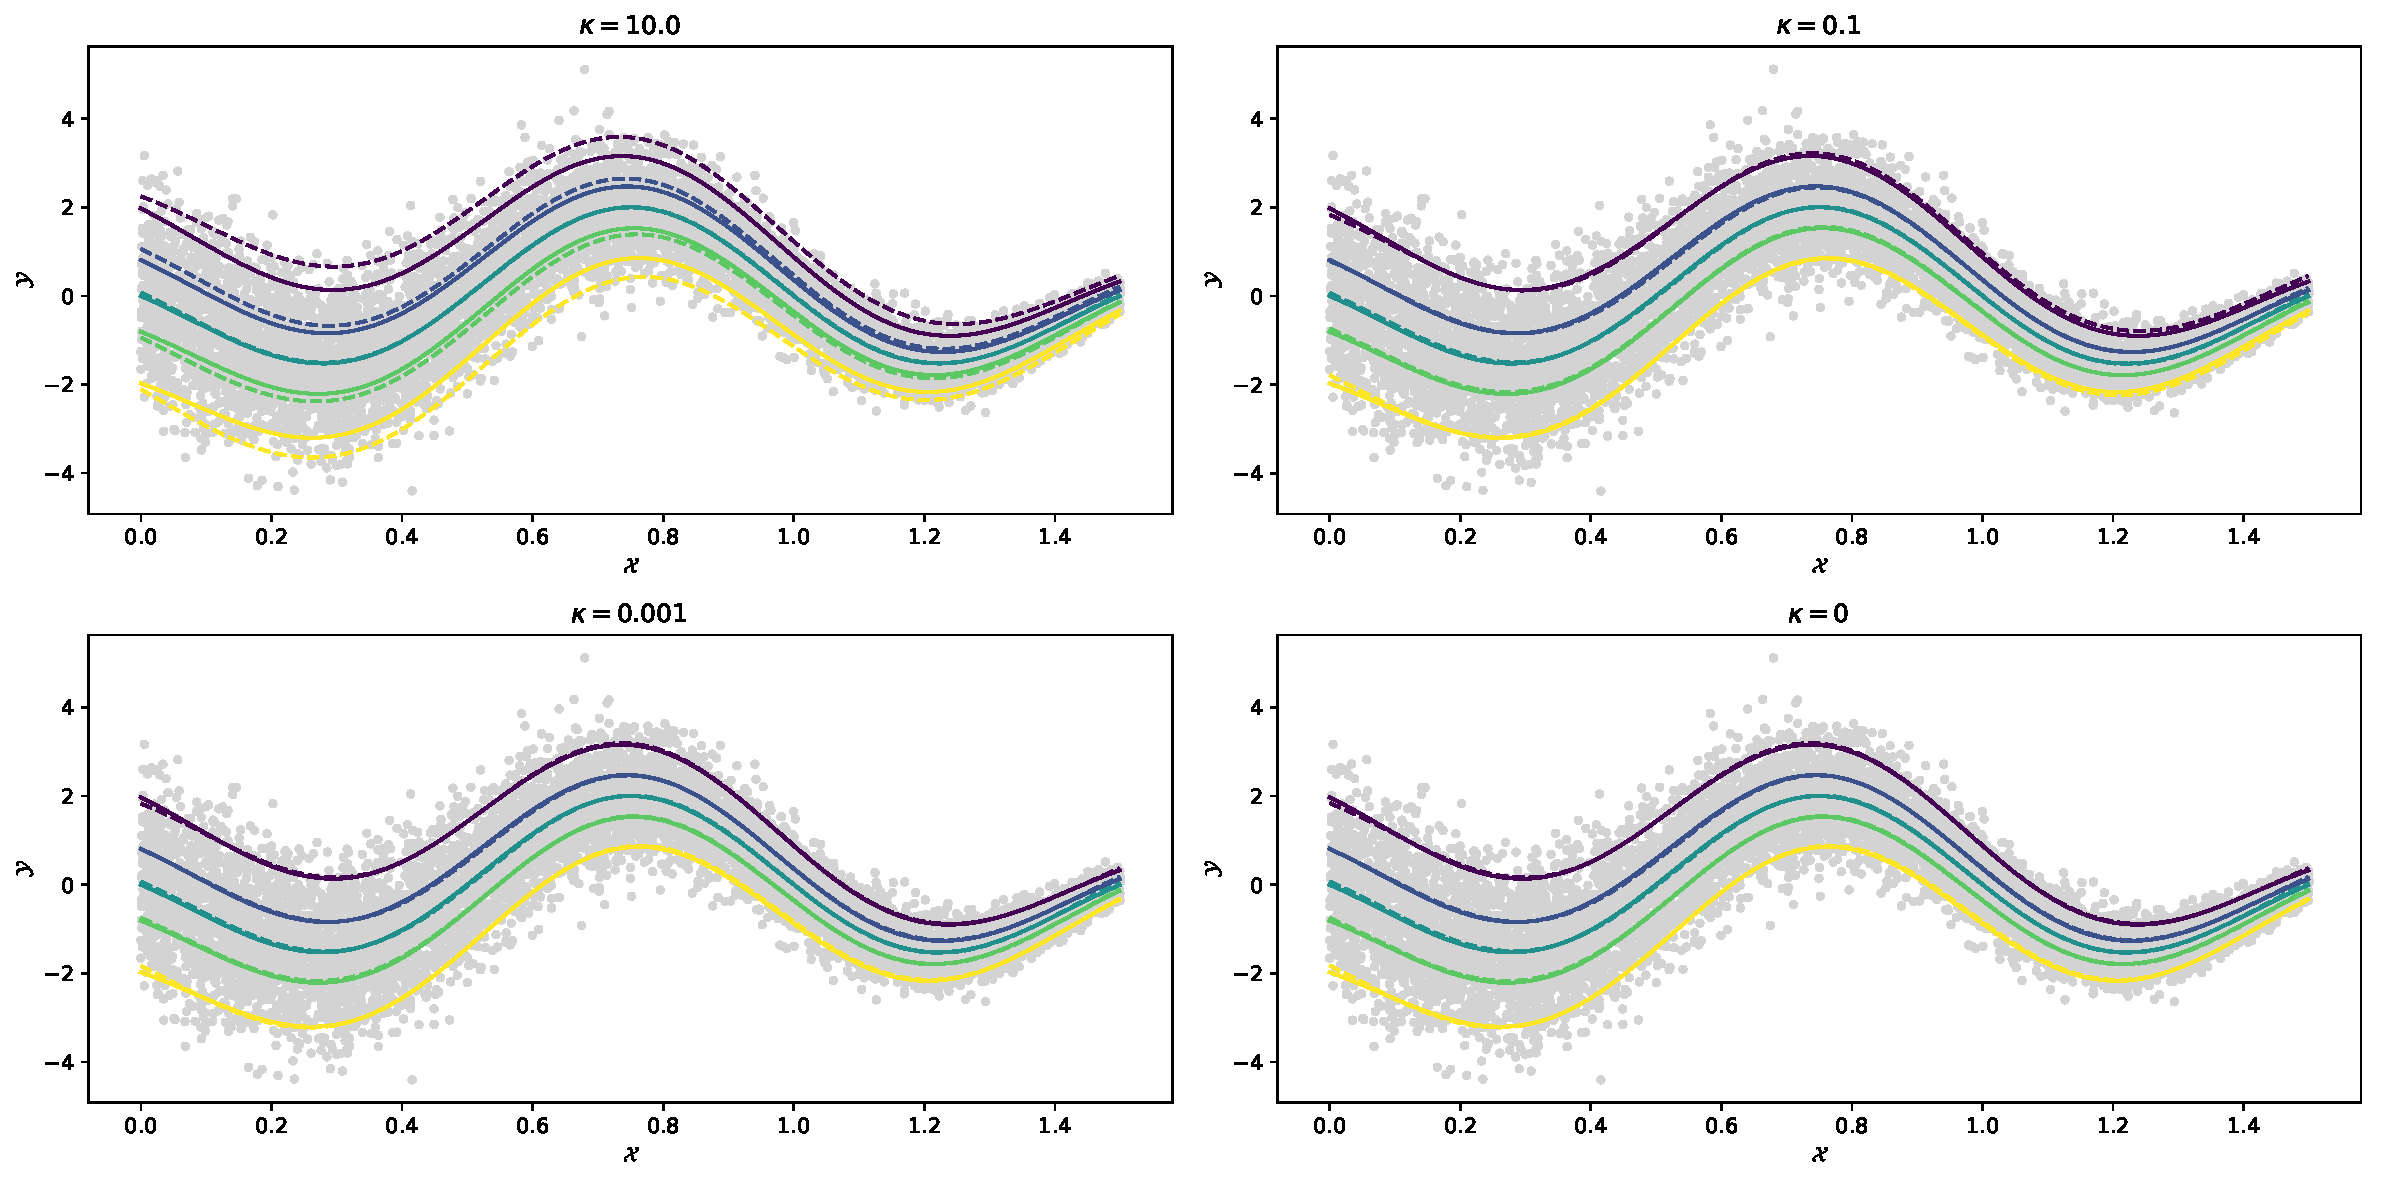
\includegraphics{src/fig/autogen/iqr_kappa.pdf}}
    \caption{Impact of the Huber loss smoothing of the pinball loss for
    differents values of $\kappa$. \label{figure:kappa_study}}
\end{figure}
\begin{table}[tb]
    \caption{Examples for objective \eqref{equation:integrated_cost}.
    $\psi_1^\kappa$, $\psi_+^\kappa$: $\kappa$-smoothed absolute value
    and positive part. $h_{x}(\hyperparameter)\defeq h(x)(\theta)$.
    \label{table:integrated_risks}}
    \begin{center}
      \addtolength{\tabcolsep}{-3pt}
      \renewcommand{\arraystretch}{0.8}
        \begin{tiny}
            \begin{sc}
                \resizebox{\textwidth}{!}{%
                \begin{tabular}{lll}
                    \toprule
                    & loss & penalty \\
                    \midrule
                    Quantile  & $\displaystyle\int_{\closedinterval{0}{1}}
                    \abs{\hyperparameter - \indicator{\reals_{-}}(y -
                    h_x(\hyperparameter))}\abs{y - h_x(\hyperparameter)}
                    d\mu(\hyperparameter)$ &
                    $\lambda_{nc}\int_{\closedinterval{0}{1}}
                    \abs{-\frac{dh_x}{d\hyperparameter}(\hyperparameter)}_+
                    d\mu(\hyperparameter) +
                    \frac{\lambda}{2}\norm{h}_{\mcH_K}^2$ \\
                    M-Quantile (smooth)  &
                    $\displaystyle\int_{\closedinterval{0}{1}}
                    \abs{\hyperparameter - \indicator{\reals_{-}}(y -
                    h_x(\hyperparameter))}\psi_1^\kappa\left(y -
                    h_x(\hyperparameter)\right)d\mu(\hyperparameter)$ &
                    $\lambda_{nc}\int_{(0, 1)} \psi_+^\kappa\left(-
                    \frac{dh_x}{d\hyperparameter}(\hyperparameter)\right)
                    d\mu(\hyperparameter) +
                    \frac{\lambda}{2}\norm{h}_{\mcH_K}^2$ \\
                    Expectiles (smooth) &
                    $\displaystyle\int_{\closedinterval{0}{1}}
                    \abs{\hyperparameter - \indicator{\reals_{-}}(y -
                    h_x(\hyperparameter))}\left(y -
                    h_x(\hyperparameter)\right)^2d\mu(\hyperparameter)$ &
                    $\lambda_{nc} \int_{(0, 1)}
                    \abs{-\frac{dh_x}{d\hyperparameter}(\hyperparameter)}_+^2
                    d\mu(\hyperparameter) +
                    \frac{\lambda}{2}\norm{h}_{\mcH_K}^2$ \\
                    Cost-Sensitive & $\displaystyle\int_{
                    \closedinterval{-1}{1}} \abs{\frac{\hyperparameter + 1}{2}
                    - \indicator{\{-1\}}(y)}\abs{1 -
                    yh_{x}(\hyperparameter)}_{+} d\mu(\theta)$ & $
                    \frac{\lambda}{2}\norm{h}_{\mcH_K}^2$ \\
                    Cost-Sensitive (smooth) &
                    $\displaystyle\int_{\closedinterval{-1}{1}}
                    \abs{\frac{\hyperparameter + 1}{2} -
                    \indicator{\{-1\}}(y)}\psi_+^\kappa\left(1 -
                    yh_{x}(\hyperparameter)\right) d\mu(\theta)$ & $
                    \frac{\lambda}{2}\norm{h}_{\mcH_K}^2$ \\
                    Level-Set   &
                    $\displaystyle\int_{\closedinterval{\epsilon}{1}}
                    -t(\hyperparameter) +
                    \frac{1}{\theta}\abs{t(\hyperparameter) -
                    h_x(\hyperparameter)}_+
                    d\mu(\hyperparameter)$ & $
                    \frac{1}{2}\displaystyle\int_{
                    \closedinterval{\epsilon}{1}}
                    \norm{h(\cdot)(\hyperparameter)}_{
                    \mcH_{k_{\inputspace}}}^2 d\mu(\hyperparameter) +
                    \frac{\lambda}{2}\norm{t}_{\mcH_{k_b}}^2$\\ \bottomrule
                \end{tabular}}
            \end{sc}
        \end{tiny}
        \addtolength{\tabcolsep}{3pt}
        \renewcommand{\arraystretch}{0.8}
    \end{center}
\end{table}
%
\subsection{Experimental protocol for \ac{QR}}  \label{subsection:proto_exp} In
this section, we give additional details regarding the choices being made while
implementing the \ac{ITL} method for $\infty$-\ac{QR}.
%
%\paragraph{Crossing Quantiles}
%The model was trained with a
%bias.  For $k_{\inputspace}$ a Gaussian kernel was used,
%$k_{\hyperparameterspace}$ and $k_{b}$ were Laplacian kernels. All bandwidths
%were set to $10$ to emphasise the possible crossings.

%\begin{dmath}\label{equation:non_crossing_constraint}
    %\Omega(h) = \lambda_{c}\sum_{i=1}^N \int_{(0, 1)} \abs{
    %-\frac{\partial}{\partial \tau} h_{\tau}(X_i)}_+ d\mu(\tau) +
    %\frac{\lambda}{2}(\norm{f}_{K}^2 + \norm{b}_{kb}^2).
%\end{dmath}
%Note that if the integral in \cref{equation:non_crossing_constraint} in uses
%the same samples $\tau_j$'s as the one used to approximate the cost function
%$\cost$, then the representer theorem applies with the expansion given in
%\cref{equation:expanded_non_crossing_constraint}.
%\begin{dmath}\label{equation:expanded_non_crossing_constraint}
    %\Omega_\lambda(h)=\lambda\sum_{j=1}^T\sum_{i=1}^N \abs{-\sum_{j'=1}^T
    %\sum_{i'=1}^N\alpha_{i'j'} k_{\inputspace}(x_i, x_{i'})\frac{\partial
    %k_{\hyperparameterspace}}{\partial\tau_j}(\tau_j, \tau_{j'}) -
    %\beta_j\frac{\partial k_b}{\partial \tau_j}(\tau_j, \tau_{j'})}_+ +
    %\sum_{i, i'=1}^N\sum_{j,
    %j'=1}^T\alpha_{ij}\alpha_{i'j'}k_{\inputspace}(x_i,
    %x_{i'})k_{\hyperparameterspace}(\tau_j,
    %\tau_{j'})+\beta_{j}\beta_{j'}k_b(\tau_j, \tau_{j'}).
%\end{dmath}
%\begin{center}
    %\begin{figure}[h]
        %% \resizebox{!}{.65\linewidth}{\includegraphics{fig/bias_experiment.eps}}
        %\caption{Model misspecification in quantile regression on the dataset
        %Engel. Left plot shows a linear model with bias and right plot without
        %bias.\label{figure:misspecified_models}}
    %\end{figure}
%\end{center}
%\par
%
\paragraph{\ac{QR} real datasets}
%
For $\infty$-\ac{QR}, $k_{\inputspace}$, $k_{\hyperparameterspace}$ were
Gaussian kernels. We set a bias term $k_b=k_{\hyperparameterspace}$. The
hyperparameters optimized were $\lambda$, the weight of the ridge penalty,
$\sigma_\inputspace$, the input kernel parameter, and
$\sigma_\hyperparameterspace=\sigma_b$, the output kernel parameter. They were
optimized in the (log)space of $\closedinterval{10^{-6}}{10^{6}}^3$. The
non-crossing constraint $\lambda_{nc}$ was set to $1$. The model was trained on
the continuum $\Theta=\openinterval{0}{1}$ using QMC and Sobol sequences. For
all datasets we draw $m=100$ quantiles form a Sobol sequence \par
%
For \ac{JQR} we similarly chose two Gaussian kernels. The optimized
hyperparameters were the same as for $\infty$-\ac{QR}.
% are also the bandwidth of the Gaussian kernel acting on the inputs, the bandwith
% of the kernel acting on the outputs, and the regularization tradeoff $\lambda$
% which where optimized in the (log)space $\closedinterval{10^{-6}}{10^{6}}^3$.
The quantiles learned were $\theta\in\Set{0.1, 0.3, 0.5, 0.7, 0.9}$.

For the IND-\ac{QR} baseline, we trained independently a non-paramatric
quantile estimator as described in \citet{takeuchi2006nonparametric}. A
Gaussian kernel was used and its bandwidth was optimized in the (log)space of
$\closedinterval{10^{-6}}{10^6}$. No non-crossing was enforced. \par
%
% \paragraph{Impact of the $\mcH_{k_{\hyperparameterspace}}$ kernel}
% See \cref{figure:gamma_t_study}.
% \begin{center}
%     \begin{figure}
%         % \resizebox{!}{.5\linewidth}{\includegraphics{fig/gamma_t_study.eps}}
%         \caption{Impact of the hyperparameter $\gamma_{\tau}$ on the
%         hyperparameter kernel $k_{\hyperparameterspace}$. Top row shows models
%         with a bias terms for $\gamma_{\tau}\in\Set{0.1, 100}$
%         respectfully left to right.  Bottom row shows the same for models
%         without bias.}
%     \label{figure:gamma_t_study}
%     \end{figure}
% \end{center}
\subsection{Experiments with \ac{CSC}}
\label{subsection:csc_expe}
In this section we provide numerical illustration concerning the \ac{CSC} problem.
We used the Iris \acs{UCI} dataset with $4$ attributes and $150$
samples, the two synthetic \textsc{scikit-learn}
\citep{pedregosa2011scikit} datasets \textsc{Two-Moons} (noise=$0.4$) and
$\textsc{Circles}$ (noise=$0.1$) with both $2$ attributes and $1000$
samples and a third synthetic \textsc{scikit-learn} dataset \textsc{Toy}
(class sep=$0.5$) with $20$ features ($4$ redundant and $10$ informative)
and $n=1000$ samples.\par
%
As detailed in \cref{section:infinite_tasks}, \acl{CSC} on a continuum
$\hyperparameterspace = \closedinterval{-1}{1}$ that we call \ac{ICSC}
can be tackled by our proposed technique.  In this case, the hyperparameter
$\hyperparameter$ controls the tradeoff between the importance of the correct
classification with labels $-1$ and $+1$. When $\hyperparameter = -1$,
class $-1$ is emphasized; the probability of correctly classified instances
with this label (called specificity) is desired to be $1$.  Similarly, for
$\hyperparameter = +1$, the probability of correct classification of samples
with label $+1$ (called sensitivity) is ideally $1$.\par
%
To illustrate the advantage of (infinite) joint learning we used two synthetic
datasets \textsc{Circles} and \textsc{Two-Moons} and the \acs{UCI}
\textsc{Iris} dataset. We chose $k_{\inputspace}$ to be a Gaussian kernel with
bandwidth $\sigma_{\inputspace}=(2\gamma_{\inputspace})^{(-1/2)}$ the median of
the Euclidean pairwise distances of the input points \citep{jaakkola1999using}.
$k_{\hyperparameterspace}$ is also a Gaussian kernel with bandwidth
$\gamma_{\hyperparameterspace}=5$.  We used $m=20$ for all datasets.
%
As a baseline we trained independently 3 \acl{CSC} classifiers with
$\hyperparameter\in\Set{-0.9,0, 0.9}$. We repeated $50$ times a random $50-50\%$
train-test split of the dataset and report the average test error and standard
deviation (in terms of sensitivity and specificity) \par
%
Our results are illustrated in \cref{table:csc_results}. For $\theta=-0.9$, both
 independent and joint learners give the desired $100\%$ specificity; the
joint \acl{CSC} scheme however has significantly higher sensitivity value
($15\%$ vs $0\%$) on the dataset \textsc{Circles}. Similar conclusion holds for the
$\theta=+0.9$ extreme: the ideal sensitivity is reached by both techniques, but
the joint learning scheme performs better in terms of specificity ($0\%$ vs
$12\%$) on the dataset \textsc{Circles}. \par
%
\begin{table*}[!htbp]
    \caption{\acs{ICSC} vs Independent (IND)-\acs{CSC}. Higher is
    better.\label{table:csc_results}}
    \addtolength{\tabcolsep}{-3pt}
    \renewcommand{\arraystretch}{0.8}% Tighter
    \begin{center}
        \begin{tiny}
            \begin{sc}
                \resizebox{.7\textwidth}{!}{%
                \begin{tabular}{cccccccc}
                    \toprule
                    \multirow{2}{*}{Dataset} & \multirow{2}{*}{Method} &
                    \multicolumn{2}{c}{$\theta=-0.9$} &
                    \multicolumn{2}{c}{$\theta=0$} &
                    \multicolumn{2}{c}{$\theta=+0.9$} \\
                    \cmidrule(lr){3-4} \cmidrule(lr){5-6} \cmidrule(lr){7-8} &
                    & \textsc{sensitivity} & \textsc{specificity} &
                    \textsc{sensitivity} & \textsc{specificity} &
                    \textsc{sensitivity} & \textsc{specificity} \\
                    \midrule
                    \multirow{ 2}{*}{\textsc{Two-Moons}} & IND &
                    $0.3\pm0.05$ & $0.99\pm0.01$ & $0.83\pm0.03$ &
                    $0.86\pm0.03$ & $0.99\pm0$ & $0.32\pm0.06$ \\
                                                & \acs{ICSC} & $0.32\pm0.05$ &
                    $0.99\pm0.01$ & $0.84\pm0.03$ & $0.87\pm0.03$ & $1\pm0$ &
                    $0.36\pm0.04$  \\
                    \multirow{ 2}{*}{\textsc{Circles}} & IND & $0\pm0$
                    & $1\pm0$ & $0.82\pm0.02$ & $0.84\pm0.03$ & $1\pm0$ &
                    $0\pm0$ \\
                                              & \acs{ICSC} & $0.15\pm0.05$ &
                    $1\pm0$ & $0.82\pm0.02$ & $0.84\pm0.03$ & $1\pm0$ &
                    $0.12\pm0.05$  \\
                    \multirow{ 2}{*}{\textsc{Iris}} & IND &
                    $0.88\pm0.08$ & $ 0.94\pm0.06$ & $0.94\pm0.05$ &
                    $0.92\pm0.06$ & $0.97\pm0.05$ & $0.87\pm0.06$\\
                                           & \acs{ICSC} & $0.89\pm0.08$ &
                    $0.94\pm0.05$ & $0.94\pm0.06$ & $0.92\pm0.05$ &
                    $0.97\pm0.04$ & $0.90\pm0.05$
                    \\
                    \multirow{ 2}{*}{\textsc{Toy}} & IND &
                    $0.51\pm0.06$ & $ 0.98\pm0.01$ & $0.83\pm0.03$ &
                    $0.86\pm0.03$ & $0.97\pm0.01$ & $0.49\pm0.07$\\
                                           & \acs{ICSC} & $0.63\pm0.04$ &
                    $0.96\pm0.01$ & $0.83\pm0.03$ & $0.85\pm0.03$ &
                    $0.95\pm0.02$ & $0.61\pm0.04$
                    \\
                    \bottomrule
                \end{tabular}}
            \end{sc}
        \end{tiny}
    \end{center}
    \addtolength{\tabcolsep}{3pt}
    \renewcommand{\arraystretch}{1.0}% Tighter
\end{table*}
% \subsubsection{Illustration of the \ac{CSC} datasets}
% \begin{figure}[!htbp]
% \setlength\fboxsep{0pt}\setlength\fboxrule{0.75pt}
% \ffigbox[\textwidth]
% {
% \begin{subfloatrow}[2]
% %\fbox{
% \ffigbox[.49\textwidth]
%   {
%     \caption{\textsc{Circle} dataset}
%     \label{subfigure:csc_circle}
%   }
%   {
%     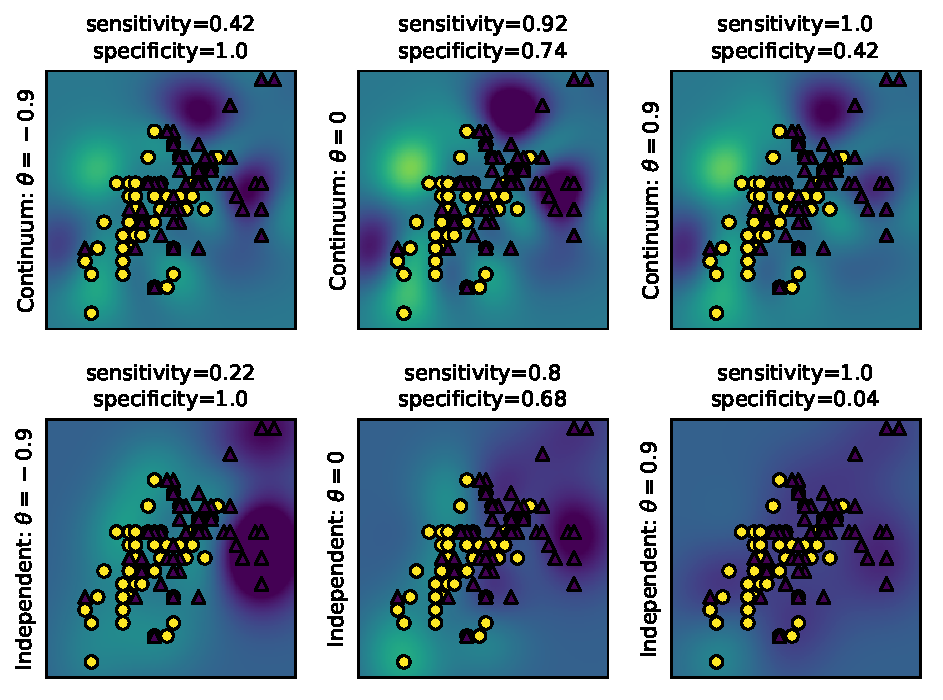
\includegraphics[angle=-90,width=\linewidth]{src/fig/autogen/icsl_vs.pdf}%
%   }
% %}
% %\fbox{
% \ffigbox[.4825\textwidth]
%   {
%     \caption{\textsc{Two-Moons} dataset}
%     \label{subfigure:csc_moons}
%   }
%   {
%     \includegraphics[angle=-90,width=\linewidth]{src/fig/autogen/icsl_vs_moons.pdf}%
%   }
% %}
% \end{subfloatrow}%
% }
% {
%     \caption{Illustration of some datasets used in \cref{table:csc_results}.
%     \label{figure:csc_datasets}}
% }
% \end{figure}%
% \textsc{Two-Moons} and \textsc{Circles} used in \cref{table:csc_results}.

%
%%%%%%%%%%%%%%%%%%%%%%%%%%%%%%%%%%%%%%%%%%%%%%%%%%%%%%%%%%%%%%%%%%%%%%%%%%%%%%%
%
%\section{Discussion}
%\input{discussion.tex}
\section{Conclusion}
\label{section:conclusion}
In this work we proposed Infinite Task Learning, a novel nonparametric framework
aiming at jointly solving parametrized tasks for a continuum of
hyperparameters.
% The approach relies on \ac{vv-RKHS}, in specific cases it recovers several
% existing multi-task approaches and extends Parametric-Task Learning to nonparametric models and a
% larger class of loss functions.
We provided
excess risk guarantees for the studied ITL scheme, and
demonstrated its practical efficiency and flexibility in various
tasks including cost-sensitive classification, quantile regression and density
     level set estimation.
% Future works should
%  study whether local properties of the algorithm ($\theta$-property in \ac{OCSVM},
%  quantile property in \ac{QR}) are asymptotically kept true for all hyperparameter values,
% as well as investigate acceleration schemes based on kernel approximations.
%
%  especially the ones outside the locations taken in the approximation of the
% integral.
% % %
% Another topic of interest concerns the exploration of other parametrized
% tasks, including ones with more complex or higher dimensional hyperparameter
% spaces.

%
%%%%%%%%%%%%%%%%%%%%%%%%%%%%%%%%%%%%%%%%%%%%%%%%%%%%%%%%%%%%%%%%%%%%%%%%%%%%%%%
%
\section*{Acknowledgments}
The authors thank Arthur Tenenhaus for some insightful discussions. This work
was supported by the Labex \emph{DigiCosme} (project ANR-11-LABEX-0045-DIGICOSME)
 and the industrial chair \emph{
Machine Learning for Big Data} at T\'el\'ecom ParisTech.

%\afterpage{\clearpage}%
%\renewcommand*{\bibfont}{\scriptsize}
\printbibliography
\clearpage
\onecolumn
\part*{SUPPLEMENTARY MATERIAL}
\renewcommand{\thesection}{S.\arabic{section}}
\renewcommand{\thesubsection}{S.\arabic{section}.\arabic{subsection}}
\renewcommand{\thesubsubsection}{S.\arabic{section}.\arabic{subsection}%
    .\arabic{subsubsection}}
\renewcommand{\thetable}{S.\arabic{table}}
\renewcommand{\thefigure}{S.\arabic{figure}}
%
%%%%%%%%%%%%%%%%%%%%%%%%%%%%%%%%%%%%%%%%%%%%%%%%%%%%%%%%%%%%%%%%%%%%%%%%%%%%%%%
%<<<<<<< HEAD
%%
%\ifthenelse{\NOT\isundefined{\draft}\OR\NOT\isundefined{\final}}{
{\centering
\subsubsection*{Acronyms}
\printacronyms[heading=none]\par}
%}{}
%%
%\\
%Below we provide the proofs of our results stated in the main part of the paper.
%=======
Below we provide the proofs of the results stated in the main part of the
paper.
%>>>>>>> 1a53644efbc9773324384e46e5d2a47af752482e
\begin{refsection}
\section{Quantile Regression}
\label{appendix:qr}
Let us recall the expression of the pinball loss \seep{figure:pinball}:
\begin{dmath}[compact]
    v_{\hyperparameter}: (y,\,y') \in
    \reals^2 \mapsto  \max{(\hyperparameter (y-y'), (\hyperparameter
    -1)(y-y'))} \in \reals.
\end{dmath}
\begin{floatingfigure}{.7\textwidth}
    \centering
    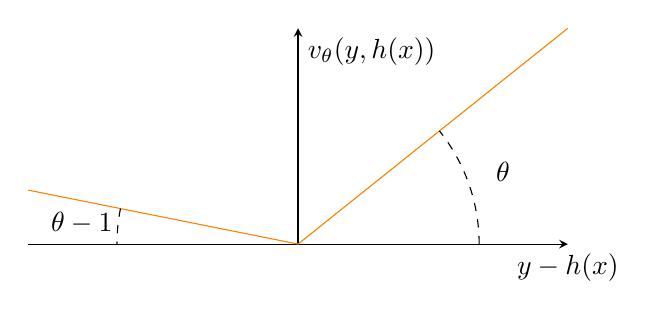
\begin{tikzpicture}
    \begin{axis}[%
        axis x line = center,
        axis y line = center,
        disabledatascaling,
        axis equal image,
        xlabel = {$y - h(x)$},
        ylabel = {$v_{\theta}(y, h(x))$},
        x label style={at={(axis description cs:1.0, 0.0)}, anchor=north},
        ticks = none
        ]
        \addplot[orange, domain=-1:1, samples at={-1, 0, 1}]
            {abs(.8 - (x < 0)) * abs(x)};
        \draw
            (-0.5, 0.1) coordinate (a)
            (0, 0) coordinate (b)
            (-0.5, 0) coordinate (c);
        \draw
            pic["$\theta - 1$", draw=black, -,dashed, angle eccentricity=1.2,
                angle radius=2.3cm]
            {angle=a--b--c};
        \draw
            (0.5, 0.4) coordinate (d)
            (0, 0) coordinate (e)
            (0.5, 0) coordinate (f);
        \draw
            pic["$\theta$", draw=black, -,dashed, angle eccentricity=1.2,
                angle radius=2.3cm]
            {angle=f--e--d};
    \end{axis}
\end{tikzpicture}

    \caption{\label{figure:pinball} Pinball loss for $\hyperparameter=0.8$.}
\end{floatingfigure}
\begin{proposition}\label{proposition:generalized_excess_risk}
    Let $X,Y$ be two \acp{rv} respectively taking values in $\mcX$ and
    $\reals$, and $q \colon \mcX \to \mathcal{F}([0,1],\mathbb{R})$ the
    associated conditional quantile function.  Let $\mu$ be a positive measure
    on $[0,1]$ such that $ \int_{0}^1 \expectation\left[
    v_{\hyperparameter}\left(Y,q(X)(\hyperparameter)\right)\right] \mathrm{d}
    \mu(\hyperparameter) < \infty$.  Then for $\forall h \in
    \functionspace{\mathcal{X}}{\functionspace{\closedinterval{0}{1}}{\reals}}$
    \begin{dmath*}
        \risk(h) - \risk(q) \geq 0,
    \end{dmath*}
    where $R$ is the risk defined in \cref{equation:h-objective}.
\end{proposition}
\begin{proof}
    The proof is based on the one given in \citep{li2007quantile} for a single
    quantile. Let $f \in
    \functionspace{\mcX}{\functionspace{\closedinterval{0}{1}}{\reals}}$,
    $\hyperparameter \in (0,1)$ and $(x,y) \in \mcX \times \reals$. Let also
    \begin{align*}
        s &=
        \begin{cases}
            1 ~ \text{if } y \leq f(x)(\hyperparameter)      \\
            0  \text{ otherwise}
        \end{cases},&
        t &=
        \begin{cases}
            1 ~ \text{if } y \leq q(x)(\hyperparameter)      \\
            0  \text{ otherwise}
        \end{cases}.
    \end{align*}
    It holds that
    \begin{dmath*}
        v_{\hyperparameter}(y,h(x)(\hyperparameter)) -
        v_{\hyperparameter}(y,q(x)(\hyperparameter))
        = \hyperparameter(1-s)(y-h(x)(\hyperparameter)) + (\hyperparameter -
        1)s(y-h(x)(\hyperparameter)) -
        \hyperparameter(1-t)(y -q(x)(\hyperparameter)) -
        (\hyperparameter-1)t(y-q(x)(\hyperparameter))
        = \hyperparameter(1-t)(q(x)(\hyperparameter) - h(x)(\hyperparameter)) +
        \hyperparameter((1-t)-(1-s))h(x)(\hyperparameter) +
        (\hyperparameter-1)t(q(x)(\hyperparameter - h(x)(\hyperparameter))) +
        (\hyperparameter-1)(t-s)h(x)(\hyperparameter) + (t-s)y\nonumber
        =     (\hyperparameter -t)(q(x)(\hyperparameter) -
        h(x)(\hyperparameter)) +
        (t-s)(y-h(x)(\hyperparameter)).\label{eq:decompo_pinball}
    \end{dmath*}
    Then, notice that
    \begin{dmath*}[compact]
        \expectation{[(\hyperparameter - t)(q(X)(\hyperparameter) -
        h(X)(\hyperparameter))]} =
        \expectation{[\expectation{[(\hyperparameter - t)(q(X)(\hyperparameter)
        - h(X)(\hyperparameter))]} | X]} =
        \expectation{[\expectation{[(\hyperparameter - t) | X ]}
        (q(X)(\hyperparameter) - h(X)(\hyperparameter))]}
    \end{dmath*}
    and since $q$ is the true quantile function,
    \begin{align*}
        \expectation{ [t | X]} = \expectation{ [\mathbf{1}_{\{ Y \leq
        q(X)(\hyperparameter)\}} | X]} = \probability{[Y \leq
        q(X)(\hyperparameter) | X]} = \hyperparameter,
    \end{align*}
    so
    \begin{align*}
        \expectation{[(\hyperparameter - t)(q(X)(\hyperparameter) -
        h(X)(\hyperparameter))]} =0.
    \end{align*}
    Moreover, $(t-s)$ is negative when $q(x)(\hyperparameter) \leq y \leq
    h(x)(\hyperparameter)$, positive when $h(x)(\hyperparameter) \leq y \leq
    q(x)(\hyperparameter)$ and $0$ otherwise, thus the quantity
    $(t-s)(y-h(x)(\hyperparameter))$ is always positive. As a consequence,
    \begin{dmath*}[compact]
        R(h) - R(q) = \int_{[0,1]}
        \expectation{[v_{\hyperparameter}(Y,h(X)(\hyperparameter)) -
        v_{\hyperparameter}(Y,q(X)(\hyperparameter))]} \mathrm{d}
        \mu(\hyperparameter) \geq 0
    \end{dmath*}
    which concludes the proof.
\end{proof}
The \cref{proposition:generalized_excess_risk} allows us to derive conditions
under which the minimization of the risk above yields the true quantile
function. Under the assumption that (i) $q$ is continuous (as seen as a
function of two variables), (ii) $\mathrm{Supp}(\mu) = [0,1] $, then the
minimization of the integrated pinball loss performed in the space of
continuous functions yields the true quantile function on the support of
$\probability_{X,Y}$.


\section{Representer Propositions}
\label{appendix:representer}
\begin{proof} [Proof of \cref{theorem:representer_supervised}]
    First notice that
    \begin{align}
        J: h \in \mcH_K \mapsto \frac{1}{n} \displaystyle\sum_{i=1}^n
        \displaystyle\sum_{j=1}^m w_j\hcost(\hyperparameter_j,y_i,
        h(x_i)(\hyperparameter_j)) + \frac{\lambda}{2} \norm{h}_{\mcH_K}^2 \in
        \reals
    \end{align}
    is a proper lower semicontinuous strictly convex function
    \citep[Corollary 9.4]{bauschke2011convex}, hence $J$ admits a unique
    minimizer $h^* \in \mcH_K$ \citep[Corollary 11.17]{bauschke2011convex}.
    Let
    \begin{dmath}[compact] \label{decompo_theorem}
        \mcU = \sspan{ \Set{
        (K(\cdot,x_i)k_{\Theta}(\cdot,\theta_j))_{i,j=1}^{n,m} | \forall  x_i
        \in \inputspace , \forall \theta_j \in \hyperparameterspace }} \subset
        \mcH_K.
    \end{dmath}
    Then $\mcU$ is a finite-dimensional subspace of $\mcH_K$, thus closed in
    $\mcH_K$, and it holds that $\mcU \oplus \mcU^{\perp} = \mcH_K$, so $h^*$
    can be decomposed as $h^* = h_{\mcU}^* + h_{\mcU^{\perp}}^*$ with
    $h_{\mcU}^* \in \mcU$ and $h_{\mcU^{\perp}}^* \in \mcU^{\perp}$. Moreover,
    for all $1 \leq i \leq n$ and $1 \leq j \leq m$,
    \begin{align*}
        h_{\mcU^{\perp}}^*(x_i)(\theta_j) &= \langle h_{\mcU^{\perp}}^*(x_i) ,
        k_{\Theta}(\cdot,\theta_j) \rangle_{\mcH_{k_{\Theta}}}
        = \langle h_{\mcU^{\perp}}^* , K(\cdot,x_i)k_{\Theta}(\cdot,\theta_j)
        \rangle_{\mcH_K}
        = 0,
    \end{align*}
    so $J(h^*) = J(h_{\mcU}^*) + \lambda \norm{h_{\mcU^{\perp}}^*}_{\mcH_K}^2$.
    However $h^*$ is the minimizer of J, therefore $h_{\mcU^{\perp}}^*=0$ and
    there exist $\left(\alpha_{ij}\right)_{i,j = 1}^{n,m}$ such that $\forall
    x,\hyperparameter \in \mcX \times \hyperparameterspace$,
    $h^*(x)(\hyperparameter) = \sum_{i,j=1}^{n,m} \alpha_{ij} k_{\mcX}(x,x_i)
    k_{\hyperparameterspace}(\hyperparameter,\hyperparameter_j)$.
    % Remark \citep{carmeli06vector} that $\mcH_K$ is isometric to the real RKHS
    %  $\mcH_{k_{\mcX}\times k_{\Theta}}$ thanks to the isometry
    %  \begin{dmath*}
    %    V \colon
    %    \begin{cases}
    %        \mcH_K & \to ~ \mcH_{k_{\mcX}\times k_{\Theta}}       \\
    %        h  & \mapsto (x,\theta \mapsto h(x)(\theta))
    %    \end{cases}
    %  \end{dmath*}
    %   Let $g^* = V(h^*)$, and define
    %   \begin{dmath*}[compact]
    %   \mcV = \sspan{ \left \{
    %   (k_{\mcX}(x_i,\cdot)k_{\Theta}(\theta_j,\cdot))_{i,j=1}^{n,m} \right \}}
    %   \subset \mcH_{k_{\mcX}\times k_{\Theta}}
    %   \end{dmath*}
      % $\mcU$ is a finite dimensional subspace of $\mcH_{k_{\mcX}\times k_{\Theta}}$,
      % thus closed, and $\mcV \oplus \mcV^{\perp} = \mcH_{k_{\mcX}\times k_{\Theta}}$,
      % so that we can write $g^* = g_{\mcV}^* + g_{\mcV^{\perp}}^*$ with $g_{\mcV}^* \in \mcV$
      % and $g_{\mcV^{\perp}}^* \in \mcV^{\perp}$. By construction,
      % \begin{dmath*}
      %   \widetilde{R}_{\mcS}(h^*) = \frac{1}{nm} \sum_{i,j=1}^{n,m}
      %   \parametrizedcost{\hyperparameter_j}(y,h^*(x_i)(\hyperparameter_j)) +
      %    \lambda \norm{h^*}_{\mcH_K}^2
      %   =\frac{1}{nm} \sum_{i,j=1}^{n,m}
      %    \parametrizedcost{\hyperparameter_j}(y,g^*(x_i,\hyperparameter_j)) +
      %    \lambda \norm{g^*}_{\mcH_{k_{\mcX}\times k_{\Theta}}}^2
      %    = \frac{1}{nm} \sum_{i,j=1}^{n,m}
      %    \parametrizedcost{\hyperparameter_j}(y,g_{\mcV}^*(x_i,\hyperparameter_j)) +
      %    \lambda (\norm{g_{\mcV}^*}_{\mcH_{k_{\mcX}\times k_{\Theta}}}^2 +
      %    \norm{g_{\mcV^{\perp}}^*}_{\mcH_{k_{\mcX}\times k_{\Theta}}}^2)
      % \end{dmath*}
      % since
    \paragraph{Derivative shapes constraints:}
    Reminder: for a function $h$ of one variable, we denote $\partial h$ the
    derivative of $h$. For a function $k(\theta, \theta')$ of two variables we
    denote $\partial_1 k$ the derivative of $k$ with respect to $\theta$ and
    $\partial_2 k$ the derivative of $k$ with respect to $\theta'$.
    %
    From \citet{zhou2008derivative}, notice that if $f\in\mathcal{H}_k$, where
    $\mathcal{H}_k$ is a scalar-valued \ac{RKHS} on a compact subset
    $\hyperparameterspace$ of $\reals^d$, and $k\in
    \mathcal{C}^{2}(\hyperparameterspace \times \hyperparameterspace)$ (in the
    sense of \citet{ziemer2012weakly}) then $\partial f\in\mathcal{H}_k$. Hence
    if one add a new term of the form:
    \begin{dmath*}
        \lambda_{\text{nc}} \sum_{i=1}^n\sum_{j=1}^m \Omega_{\text{nc}}
        \left(\left(\partial\left[h(x_i)\right]\right)(\theta_j)\right) =
        \lambda_{\text{nc}}\sum_{i=1}^n\sum_{j=1}^m
        \Omega_{\text{nc}}\left((\partial h(x_i))(\theta_j)\right)
    \end{dmath*}
    where $g$ is a strictly monotonically increasing function and
    $\lambda_{\text{nc}} > 0$, a new representer theorem can be obtained by
    constructing the new set
    \begin{dmath*}[compact] 
        \mcU = \sspan{ \Set{
        (K(\cdot,x_i)k_{\Theta}(\cdot,\theta_j))_{i,j=1}^{n,m} | \forall  x_i
        \in \inputspace , \forall \theta_j \in \hyperparameterspace }
        \cup \Set{
        (K(\cdot,x_i)(\partial_2 k_{\Theta})(\cdot,\theta_j))_{i,j=1}^{n,m} |
        \forall  x_i \in \inputspace , \forall \theta_j \in
        \hyperparameterspace }
        }
        \subset
        \mcH_K.
    \end{dmath*}
    The proof is the same as \cref{theorem:representer_supervised} with the
    new set $\mathcal{U}$ to obtain the expansion $h(x)(\theta) =
    \sum_{i=1}^n\sum_{j=1}^m \alpha_{ij} k_{\inputspace}(x,
    x_i)k_{\hyperparameterspace}(\theta, \theta_j) + \beta_{ij}k(x,
    x_i)(\partial_2k_{\hyperparameterspace})(\theta, \theta_j)$.  For the
    regularization notice that for a symmetric function $(\partial_1 k)(\theta,
    \theta') = (\partial_2 k)(\theta', \theta)$. Hence $\inner{(\partial_1
    k)(\cdot, \theta'), k(\cdot, \theta)}_{\mathcal{H}_k} = \inner{k(\cdot,
    \theta'), (\partial_2 k)(\cdot, \theta)}_{\mathcal{H}_k}$ and $(\partial
    k_{\theta'})(\theta) = (\adjoint{\partial} k_{\theta})(\theta')$ and
    \begin{dmath*}
        \norm{h}_{\mathcal{H}_K}^2
        = \inner{h, h}_{\mathcal{H}_K}
        = \sum_{i=1}^n\sum_{j=1}^m\sum_{i'=1}^n\sum_{j'=1}^m
        \alpha_{ij}\alpha_{i'j'}k_{\inputspace}(x_i,
        x_{i'})k_{\hyperparameterspace}(\theta_j, \theta_{j'}) +
        \alpha_{ij}\beta_{i'j'}k_{\inputspace}(x_i, x_{i'})(\partial_2
        k_{\hyperparameterspace})(\theta_j, \theta_{j'}) +
        \alpha_{i'j'}\beta_{ij}k_{\inputspace}(x_i, x_{i'})(\partial_1
        k_{\hyperparameterspace})(\theta_j, \theta_{j'}) +
        \beta_{ij}\beta_{i'j'}k_{\inputspace}(x_i,
        x_{i'})(\partial_1\partial_2k_{\hyperparameterspace})(\theta_j,
        \theta_{j'})
    \end{dmath*}
    Eventually $(\partial h(x))(\theta) = \sum_{i=1}^n\sum_{j=1}^m \alpha_{ij}
    k_{\inputspace}(x, x_i)(\partial_1 k_{\hyperparameterspace})(\theta,
    \theta_j) + \beta_{ij}k(x,
    x_i)(\partial_1\partial_2k_{\hyperparameterspace})(\theta, \theta_j)$.
\end{proof}
To prove \cref{theorem:representer_ocsvm}, the following lemmas are useful.
\begin{lemma} \citep{carmeli10vector} \label{lemma:isometry}
    Let $k_{\mcX}:\inputspace \times \inputspace \rightarrow \reals$,
    $k_{\hyperparameterspace}:\hyperparameterspace \times \hyperparameterspace
    \rightarrow \reals$ be two scalar-valued kernels and $K (\theta',\theta) =
    k_{\hyperparameterspace}(\theta,\theta')I_{\mcH_{k_{\mcX}}}$.  Then $H_K$
    is isometric to $\mcH_{k_{\mcX}} \otimes \mcH_{k_{\hyperparameterspace}}$
    by means of the isometry $W: f \otimes g \in \mcH_{k_{\mcX}} \otimes
    \mcH_{k_{\hyperparameterspace}} \mapsto ( \hyperparameter \mapsto
    g(\hyperparameter)f) \in \mcH_K$.
\end{lemma}
%
\begin{remark}
    Given $k_{\mcX}:\inputspace \times \inputspace \rightarrow \reals$,
    $k_{\hyperparameterspace}:\hyperparameterspace \times \hyperparameterspace
    \rightarrow \reals$ two scalar-valued kernels, we define $K:(x,z) \in \mcX
    \times \mcX \mapsto k_{\mcX}(x,z) I_{\mcH_{k_{\hyperparameterspace}}} \in
    \mathcal{L}(\mcH_{k_{\hyperparameterspace}}  )$, $K':
    (\hyperparameter,\hyperparameter')\in \hyperparameterspace \times
    \hyperparameterspace \mapsto
    k_{\hyperparameterspace}(\hyperparameter,\hyperparameter')
    I_{\mcH_{k_{\mcX}}} \in \mathcal{L}(\mcH_{k_{\mcX}})$.
    \cref{lemma:isometry} allows us to say that $\mcH_{K}$ and $\mcH_{K'}$ are
    isometric by means of the isometry \begin{align}
    \label{equation:v_definition} W: h \in \mcH_{K'} \mapsto (x \mapsto (\theta
    \mapsto h(\theta)(x))) \in \mcH_K.  \end{align}
\end{remark}

\begin{lemma} \label{lemma:decompo_ortho}
    Let $k_{\mcX}:\inputspace \times \inputspace \rightarrow \reals$,
    $k_{\hyperparameterspace}:\hyperparameterspace \times \hyperparameterspace
    \rightarrow \reals$  be two scalar-valued kernels and $K : (\theta,\theta')
    \mapsto k_{\hyperparameterspace}(\theta,\theta')I_{\mcH_{k_{\mcX}}}$.  For
    $\hyperparameter \in \hyperparameterspace$, define $K_{\hyperparameter}: f
    \in \mcH_{k_{\mcX}} \mapsto \left ( \hyperparameter' \mapsto
    K(\hyperparameter',\hyperparameter)f \right ) \in \mcH_K$.  It is easy to
    see that $K_{\hyperparameter}^*$ is the evaluation operator
    $K_{\hyperparameter}^*: h \in \mcH_K \mapsto h(\hyperparameter) \in
    \mcH_{k_{\mcX}}$.  Then $\forall m \in \mathbb{N}^*, \forall
    (\theta_j)_{j=1}^m \in \Theta^m$,
    \begin{dmath} \label{equation:decompo_ortho}
        \left ( +_{j=1}^m \Image(K_{\theta_j}) \right) \oplus \left
        (\cap_{j=1}^m \Nullspace(K_{\theta_j} ^*) \right ) = \mcH_K
    \end{dmath}
\end{lemma}
\begin{proof}
    The statement boils down to proving that $\mcV :=\left ( +_{j=1}^m
    \Image(K_{\theta_j}) \right)$ is closed in $\mcH_K$, since it is
    straightforward that $\mcV ^{\perp} = \left (\cap_{j=1}^m \Nullspace
    \left(K_{\theta_j} ^*\right ) \right)$.  Let  $\left(e_j \right)_{j=1}^k$
    be an orthonormal basis of
    $\sspan{\Set{(k_{\hyperparameterspace}(\cdot,\hyperparameter_j))_{j=1}^m}}
    \subset \mcH_{k_{\hyperparameterspace}}$. Such basis can be obtained by
    applying the Gram-Schmidt orthonormalization method to
    $(k_{\hyperparameterspace}(\cdot,\hyperparameter_j))_{j=1}^m$. Then, $V =
    \sspan{ \Set{ e_j \cdot f , 1 \leq j \leq k, f \in \mcH_{k_{\mcX}}}}$.
    Notice also that $1 \leq j,l \leq k, \forall f,g \in \mcH_{k_{\mcX}}$,
    \begin{dmath} \label{equation:scalar_tensor} \langle e_j \cdot f, e_l \cdot
    g \rangle_{\mcH_K} = \langle e_j , e_l
    \rangle_{\mcH_{k_{\hyperparameterspace}}} \cdot \langle f,g
    \rangle_{\mcH_{k_{\mcX}}} \end{dmath} Let $(h_n)_{n \in \mathbb{N}^*}$ be a
    sequence in $\mcV$ converging to some $h \in \mcH_K$. By definition, one
    can find sequences $(f_{1,n})_{n \in \mathbb{N}^*},\ldots,(f_{k,n})_{n \in
    \mathbb{N}^*} \in \mcH_{k_{\mcX}}$ such that $\forall n \in \mathbb{N}^*$,
    $h_n = \sum_{j=1}^k e_j \cdot f_{n,j}$.  Let $p,q \in \mathbb{N}^*$. It
    holds that, using the orthonormal property of $\left(e_j \right)_{j=1}^k$
    and \cref{equation:scalar_tensor}, $\norm{h_p - h_q}_{\mcH_K}^2 = \norm{
    \sum_{j=1}^k e_j (f_{j,p} - f_{j,q})}_{\mcH_K}^2 = \sum_{j=1}^k \norm{
    f_{j,p} - f_{j,q}}_{\mcH_{k_{\mcX}}}^2$. $(h_n)_{n \in \mathbb{N}^*}$ being
    convergent, it is a Cauchy sequence, thus so are the sequences
    $(f_{j,n})_{n \in \mathbb{N}^*}$. But $\mcH_{k_{\mcX}}$ is a complete
    space, so these sequences are convergent in $\mcH_{k_{\mcX}}$, and by
    denoting $f_j = \lim_{n \to \infty} f_{j,n}$, one gets $h = \sum_{j=1}^k
    e_k \cdot f_j$.  Therefore $h \in \mcV$, $\mcV$ is closed and the
    orthogonal decomposition \cref{equation:decompo_ortho} holds.
\end{proof}
%
\begin{lemma} \label{lemma:coercivity}
    Let $k_{\mcX},k_{\hyperparameterspace}$ be two scalar kernels and $K :
    (\theta,\theta') \mapsto
    k_{\hyperparameterspace}(\theta,\theta')I_{\mcH_{k_{\mcX}}}$.  Let also $m
    \in \mathbb{N}^*$ and $(\theta_j)_{j=1}^m \in \Theta^m$, and $\mcV = \left
    ( +_{j=1}^m \Image(K_{\theta_j}) \right)$. Then  $I: \mcV \rightarrow
    \reals$ defined as $I (h) =  \sum_{j=1}^m
    \norm{h(\hyperparameter_j)}_{\mcH_{k_{\mcX}}}^2$ is coercive.
\end{lemma}
\begin{proof}
    Notice first that if there exists $\theta_j$ such that
    $k_{\hyperparameterspace}(\theta_j,\theta_j) = 0$, then
    $\Image(K_{\theta_j})=0 $, so without loss of generality, we assume that
    $k_{\hyperparameterspace}(\theta_j,\theta_j) > 0 $ ($1 \leq j \leq m$).
    Notice that $I$ is the quadratic form associated to the $L:\mcH_K
    \rightarrow \mcH_K$ linear mapping $ L (h) = \sum_{j=1}^m
    K_{\hyperparameter_j}K_{\hyperparameter_j}^*$.  Indeed, $\forall h \in
    \mcV$, $I(h) = \sum_{j=1}^m \langle
    K_{\hyperparameter_j}^*h,K_{\hyperparameter_j}^*h \rangle_{\mcH_{k_{\mcX}}}
    = \sum_{j=1}^m \langle h, K_{\hyperparameter_j}K_{\hyperparameter_j}^* h
    \rangle_{\mcH_K} = \langle h , L h \rangle_{\mcH_K}$.  Moreover, $\forall 1
    \leq j \leq m$, $K_{\hyperparameter_j}K_{\hyperparameter_j}^*$ has the same
    eigenvalues as $K_{\hyperparameter_j}^*K_{\hyperparameter_j}$, and $\forall
    f \in \mcH_{k_{\mcX}}$, $K_{\hyperparameter_j}^*K_{\hyperparameter_j} f =
    k_{\hyperparameterspace}(\hyperparameter_j,\hyperparameter_j)f$, so that
    the only possible eigenvalue is
    $k_{\hyperparameterspace}(\hyperparameter_j,\hyperparameter_j)$.  Let $h
    \in \mcV$, $h \neq 0$. Because of the \cref{equation:decompo_ortho}, $h$
    cannot be simultaneously in all $\Nullspace(K_{\hyperparameter_j}^*)$, and
    there exists $i_0$ such that $I(h) \geq
    k_{\hyperparameterspace}(\hyperparameter_{i_0},\hyperparameter_{i_0})
    \norm{h}_{\mcH_K}^2$.  Let $\gamma = \underset{1 \leq j \leq m}{\min}
    k_{\hyperparameterspace}(\hyperparameter_{j},\hyperparameter_{j})$.  By
    assumption $\gamma >0$, and it holds that $\forall h \in \mcV$, $I(h) \geq
    \gamma \norm{h}_{\mcH_K}^2$, which proves the coercivity of $I$.
\end{proof}
\begin{proof} [Proof of \cref{theorem:representer_ocsvm}]
    Let $K: (x,z) \in \mcX \times \mcX \mapsto k_{\mcX}(x,z)
    I_{\mcH_{k_{\hyperparameterspace}}} \in
    \mathcal{L}(\mcH_{k_{\hyperparameterspace}}  )$, $K':
    (\hyperparameter,\hyperparameter') \in \hyperparameterspace \times
    \hyperparameterspace \mapsto
    k_{\hyperparameterspace}(\hyperparameter,\hyperparameter')
    I_{\mcH_{k_{\mcX}}} \in \mathcal{L}(\mcH_{k_{\mcX}})$, and define
    \begin{dmath*}
        J \colon
        \begin{cases}
            \mcH_K \times \mcH_{k_{b}} & \to \mathbb{R}  \\
            (h,t)  & \mapsto   \frac{1}{n} \displaystyle\sum_{i,j=1}^{n,m}
            \frac{w_j}{\hyperparameter_j} \abs{t(\hyperparameter_j) -
            h(x_i)(\hyperparameter_j)}_{+} + \displaystyle\sum_{j=1}^m w_j
            \left (\norm{h(\cdot)(\hyperparameter_j)}_{\mcH_{k_{\mcX}}}^2 -
            t(\hyperparameter_j) \right ) + \frac{\lambda}{2}
            \norm{t}_{\mcH_{k_{b}}}^2.
        \end{cases}
    \end{dmath*}
  Let $\mcV = W \left ( +_{j=1}^m \Image(K_{\theta_j}') \right) $ where
  $W \colon \mcH_{K'} \to \mcH_K$ is defined in \cref{equation:v_definition}. Since $W$ is an isometry,
  thanks to \cref{equation:decompo_ortho}, it holds that
  $\mcV \oplus \mcV^{\perp} = \mcH_K$.
    Let $(h,t) \in \mcH_K \times \mcH_{k_{b}}$, there exists unique $ h_{\mcV^{\perp}} \in \mcV^{\perp}$,
$ h_{\mcV} \in \mcV$ such that $h = h_{\mcV} + h_{\mcV^{\perp}}$. Notice that
  $J(h,t) = J(h_{\mcV} + h_{\mcV^{\perp}},t) = J(h_{\mcV},t)$
since $\forall 1 \leq j \leq m, \forall x \in \mcX$,
$h_{\mcV^{\perp}}(x)(\hyperparameter_j) = W^{-1}h_{\mcV^{\perp}}(\hyperparameter_j)(x) = 0$.
Moreover, J is bounded by below so that its infinimum is well-defined, and
  $\underset{(h,t) \in \mcH_K \times \mcH_{k_{b}}}{\inf} J(h,t) =
  \underset{(h,t) \in \mcV \times \mcH_{k_{b}}}{\inf} J(h,t)$.
Finally, notice  that $J$ is coercive on $\mcV \times \mcH_{k_{b}}$ endowed
with the sum of the norm (which makes it a Hilbert space): if
$(h_n,t_n)_{n \in \mathbb{N}^*} \in \mcV \times \mcH_{k_{b}}$ is such that
$\norm{h_n}_{\mcH_K} + \norm{t_n}_{\mcH_{k_{b}}} \underset{n \to \infty}{\to} + \infty$,
then either $(\norm{h_n}_{\mcH_K})_{n \in \mathbb{N}}$ or
$(\norm{t_n}_{\mcH_{k_b}})_{n \in \mathbb{N}}$ has to diverge :
\begin{itemize}
  \item If $\norm{t_n}_{\mcH_{k_{b}}} \underset{n \to \infty}{\to} + \infty$,
  since
  $t_n(\theta_j) = \langle t_n, k_{b}(\cdot,\theta_j) \rangle_{\mcH_{k_{b}}}
    \leq k_{b}(\theta_j,\theta_j) \norm{t_n}_{\mcH_{k_b}} \leq
    \kappa_{b} \norm{t_n}_{\mcH_{k_b}}$ $(\forall 1 \leq j \leq m)$,
  then $J(h_n,t_n) \geq
    \frac{\lambda}{2} \norm{t_n}_{\mcH_{k_{b}}}^2 - \sum_{j=1}^m w_j t(\theta_j)
    \underset{n \to \infty}{\to} + \infty$.
  \item If $\norm{h_n}_{\mcH_{K}} \underset{n \to \infty}{\to} + \infty$,
  according to \cref{lemma:coercivity}, $J(h_n,t_n)\underset{n \to \infty}{\to} + \infty $ as long
  as all $w_j$ are strictly positive.
\end{itemize}

Thus $J$ is coercive, so that \citep[Proposition 11.15]{bauschke2011convex} allows to conclude that
$J$ has a minimizer $(h^*,t^*)$ on $\mcV \times \mcH_{k_{b}}$.
Then, in the same fashion as \cref{decompo_theorem}, define
$\mcU_1 = \sspan{\Set{
(K(\cdot,x_i)k_{\Theta}(\cdot,\theta_j))_{i,j=1}^{n,m} }}
\subset \mcV$ and
$\mcU_2 = \sspan{\Set{
(k_{b}(\cdot,\theta_j))_{j=1}^{m} }}
\subset \mcH_{k_{b}}$,
and use the reproducing property to show that $(h^*,t^*) \in \mcU_1 \times \mcU_2$,
so that there
there exist $\left(\alpha_{ij}\right)_{i,j = 1}^{n,m}$ and
$\left ( \beta_{j} \right )_{j=1}^m$ such that $\forall x,\hyperparameter \in \mcX
    \times \hyperparameterspace$,
     $h^*(x)(\hyperparameter) = \sum_{i,j=1}^{n,m} \alpha_{ij} k_{\mcX}(x,x_i)
      k_{\hyperparameter}(\hyperparameter,\hyperparameter_j)$,
      $t^*(\hyperparameter)  = \sum_{j=1}^{m} \beta_{j} k_{b}(\hyperparameter,\hyperparameter_j)$.
%     h^*(x)(\hyperparameter) = \sum_{i,j=1}^{n,m} \alpha_{ij} k_{\mcX}(x,x_i)
%     k_{\hyperparameterspace}(\hyperparameter,\hyperparameter_j)
% \end{dmath*}
% \begin{dmath*}[compact]
%     t^*(\hyperparameter) = \sum_{j=1}^{m} \beta_{j} k_{\hyperparameterspace}(\hyperparameter,\hyperparameter_j)
% \end{align*}

    % Let $h^*,t^* \in \mcH_K \times \mcH_{k_{\hyperparameterspace}}$ be the solution of the
    % minimization problem
    % \begin{dmath*}
    %     h^*,t^* \in \argmin_{h \in \mcH_K, t \in \mcH_{k_{\hyperparameterspace}}}
    %     \frac{1}{nm} \sum_{i,j=1}^{n,m} \max (t(\hyperparameter_j) - h(x_i)(\hyperparameter_j),0) +
    %     \sum_{j=1}^m \left ( \hyperparameter_j \norm{h(\cdot)(\hyperparameter_j)}_{\mcH_{k_{\mcX}}}^2 - \hyperparameter_j
    %     t(\hyperparameter_j) \right ) + \lambda \norm{t}_{\mcH_{k_{\hyperparameterspace}}}^2
    % \end{dmath*}
    % Then there exist $\left(\alpha_{ij}\right)_{i,j = 1}^{n,m}$ and
    % $\left ( \beta_{j} \right )_{j=1}^m$ such that $\forall x,\hyperparameter \in \mcX
    %     \times (0,1)$,
    % \begin{dmath*}[compact]
    %     h^*(x)(\hyperparameter) = \sum_{i,j=1}^{n,m} \alpha_{ij} k_{\mcX}(x,x_i)
    %     k_{\hyperparameterspace}(\hyperparameter,\hyperparameter_j)
    % \end{dmath*}
    % \begin{dmath*}[compact]
    %     t^*(\hyperparameter) = \sum_{j=1}^{m} \beta_{j} k_{\hyperparameterspace}(\hyperparameter,\hyperparameter_j)
    % \end{dmath*}
    % Let $h^*,t^* \in \mcH_K \times \mcH_{k_{\hyperparameterspace}}$ be the solution of
    % the aforementioned minimization problem. Since $\sspan{k_{\mcX}(\cdot,
    %         x_i)k_{\hyperparameterspace}(\cdot,\hyperparameter_j)}$ is a closed subspace of the RKHS
    % $H_{k_{\mcX} \times k_{\hyperparameterspace}}$ associated to the joint kernel
    % $k_{\mcX}k_{\hyperparameterspace}$, one can decompose
\end{proof}


\section{Generalization error in the context of stability}
\label{appendix:stability}
The analysis of the generalization error will be performed using  the notion of
uniform stability introduced in \citep{bousquet2002stability}. For a derivation
of generalization bounds in \ac{vv-RKHS}, we refer to
\citep{kadri2016operator}.  In their framework, the goal is to minimize a risk
which can be expressed as
\begin{dmath}
    R_{\trainingset,\lambda}(h) = \frac{1}{n} \sum_{i=1}^n \ell(y_i,h,x_i) +
    \lambda \norm{h}_{\mcH_K}^2,
\end{dmath}
where $\trainingset = ((x_1,y_1),\ldots,(x_n,y_n))$ are \ac{iid} inputs and
$\lambda > 0$.  We almost recover their setting by using losses defined as
\begin{dmath*}
  \ell \colon
  \begin{cases}
      \reals \times \mcH_K \times \mcX &\to ~ \mathbb{R}      \\
      (y,h,x)  & \mapsto  \widetilde{V}(y,f(x)),
  \end{cases}
\end{dmath*}
where $\widetilde{V}$ is a loss associated to some local cost defined in
\cref{equation:integrated_cost}. Then, they study the stability of the
algorithm which, given a dataset $\trainingset$, returns

\begin{dmath} \label{equation:algo}
    \minimizer{h}_{\trainingset} = \argmin_{h \in \mcH_K}
    R_{\trainingset,\lambda}(h).
\end{dmath}

There is a slight difference between their setting and ours, since they use
losses defined for some $y$ in the output space of the \ac{vv-RKHS}, but this
difference has no impact on the validity of the proofs in our case. The use of
their theorem requires some assumption that are listed below. We recall the
shape of the \ac{OVK} we use : $K: (x,z) \in \mcX \times \mcX \mapsto
k_{\mcX}(x,z) I_{\mcH_{k_{\hyperparameterspace}}} \in
\mathcal{L}(\mcH_{k_{\hyperparameterspace}})$, where $k_{\mcX}$ and
$k_{\hyperparameterspace}$ are both bounded scalar-valued kernels, in other
words there exist $(\kappa_{\mcX},\kappa_{\Theta}) \in \reals^2$ such that
$\underset{x \in \mcX}{\sup}~ k_{\mcX}(x,x) < \kappa_{\mcX}^2$ and
$\underset{\theta \in \Theta}{\sup}~ k_{\Theta}(\theta,\theta) <
\kappa_{\Theta}^2$.

\begin{assumption} \label{assumption:1}
    $\exists \kappa > 0$ such that $\forall x \in \mcX$,
    $\norm{K(x,x)}_{\mathcal{L}(\mcH_{k_{\hyperparameterspace}})} \leq
    \kappa^2$.
\end{assumption}
\begin{assumption} \label{assumption:2}
    $\forall h_1,h_2 \in \mcH_{k_{\hyperparameterspace}}$, the function
    $(x_1,x_2) \in \mcX \times \mcX \mapsto \langle K(x_1,x_2) h_1,h_2
    \rangle_{\mcH_{k_{\hyperparameterspace}}} \in \reals$ \condition{is
    measurable.}
\end{assumption}
\begin{remark}
    Assumptions \ref{assumption:1}, \ref{assumption:2} are satisfied for our
    choice of kernel.
\end{remark}
\begin{assumption} \label{assumption:3}
    The application $(y,h,x) \mapsto \ell(y,h,x)$ is $\sigma$-admissible,
    \ac{ie} convex with respect to $f$ and Lipschitz continuous with respect to
    $f(x)$, with $\sigma$ as its Lipschitz constant.
\end{assumption}
\begin{assumption} \label{assumption:4}
    $\exists \xi \geq 0$ such that $\forall (x,y) \in \mcX \times \mcY$ and
    $\forall \trainingset$  training set,
    $ \ell(y,\minimizer{h}_{\trainingset},x) \leq \xi$.
\end{assumption}
%
\begin{definition}
Let $\trainingset = \left((x_i,y_i)\right)_{i=1}^n$ be the training data.
We call $\trainingset^i$ the training data
$\trainingset^i = ((x_1,y_1),\ldots,(x_{i-1},y_{i-1}),(x_{i+1},y_{i+1}),
\ldots,(x_n,y_n))$, $ 1 \leq i \leq n$.
\end{definition}

\begin{definition}A learning algorithm mapping a dataset
    $\trainingset$ to a function $\minimizer{h}_{\trainingset}$
    is said to be $\beta$-uniformly stable with
    respect to the loss function $\ell$ if $\forall n \geq 1$,
    $\forall 1 \leq i \leq n$, $\forall \trainingset \text{ training set}$,
    $||\ell(\cdot,\minimizer{h}_{\trainingset},\cdot) -
        \ell(\cdot, \minimizer{h}_{\trainingset^{ i}},\cdot)||_{\infty}
        \leq \beta$.
\end{definition}
%
\begin{proposition} \label{proposition:bousquet_generalization}
    \citep{bousquet2002stability} Let $\trainingset \mapsto
        \minimizer{h}_{\trainingset}$ be a learning algorithm
    with uniform stability $\beta$ with respect to a loss $\ell$ satisfying
    \cref{assumption:4}. Then $\forall n \geq 1$, $\forall \delta \in (0,1)$,
    with probability at least $1-\delta$ on the drawing of the samples, it
    holds that
    \begin{dmath*}
        \risk(\minimizer{h}_{\trainingset}) \leq
        \empiricalrisk(\minimizer{h}_{\trainingset}) + 2 \beta +
        (4 \beta + \xi) \sqrt{\frac{\log{(1/\delta)}}{n}}.
    \end{dmath*}
\end{proposition}

\begin{proposition} \citep{kadri2016operator} \label{proposition:kadri}
Under assumptions
\ref{assumption:1}, \ref{assumption:2}, \ref{assumption:3}, a learning algorithm
that maps a training set $\trainingset$ to the function $\minimizer{h}_{\trainingset}$ defined in
\cref{equation:algo} is $\beta$-stable with $\beta =
\frac{\sigma^2 \kappa^2}{2 \lambda n }$.
\end{proposition}

\subsection{Quantile Regression}
We recall that in this setting, $\hcost(\hyperparameter,y,h(x)(\hyperparameter)) =
\max{(\hyperparameter(y-h(x)(\hyperparameter)),(1-\hyperparameter)(y-h(x)(\hyperparameter)))}$
and the loss is
\begin{dmath}
  \ell \colon
  \begin{cases}
      \reals \times \mcH_K \times \mcX &\to ~ \mathbb{R}      \\
      (y,h,x)  & \mapsto \frac{1}{m} \sum_{j=1}^m \max{(\theta_j(y-h(x)(\theta_j)),(\theta_j-1)(y-h(x)(\theta_j)))}.
  \end{cases}
\end{dmath}
Moreover, we will assume that $|Y|$ is bounded by $B \in \mathbb{R}$ as a \ac{rv}. We will
therefore verify the hypothesis for $y \in [-B,B]$ and not $y \in \reals$.
\begin{lemma} \label{lemma:admissibility_qr}
  In the case of the \ac{QR}, the loss $\ell$ is $\sigma$-admissible
  with $\sigma = 2 \kappa_{\hyperparameterspace}$.
\end{lemma}
\begin{proof}
  Let $h_1,h_2 \in \mcH_K$ and
  $\hyperparameter \in [0,1]$. $\forall x,y \in \mcX \times \reals$, it holds that
  \begin{dmath*}[compact]
  \hcost(\hyperparameter,y,h_1(x)(\hyperparameter)) - \hcost(\hyperparameter,y , h_2(x)(\hyperparameter)) =
  (\hyperparameter -t)(h_2(x)(\hyperparameter) - h_1(x)(\hyperparameter)) + (t-s)(y-h_1(x)(\hyperparameter)),
  \end{dmath*}
  where $s = \mathbf{1}_{y \leq h_1(x)(\hyperparameter)}$ and
  $t = \mathbf{1}_{y \leq h_2(x)(\hyperparameter)}$. We consider all possible cases for
  $t$ and $s$ :
  \begin{compactitem}
    \item $t = s = 0$ : $|(t-s)(y-h_1(x)(\hyperparameter)) |
    \leq |h_2(x)(\hyperparameter) - h_1(x)(\hyperparameter)| $
    \item $t = s = 1$ : $|(t-s)(y-h_1(x)(\hyperparameter)) |
    \leq |h_2(x)(\hyperparameter) - h_1(x)(\hyperparameter)| $
    \item $s=1$,$t=0$ : $|(t-s)(y-h_1(x)(\hyperparameter)) | = |h_1(x)(\hyperparameter) - y| \leq
     |h_1(x)(\hyperparameter) - h_2(x)(\hyperparameter)| $
    \item $s=0$,$t=1$ : $|(t-s)(y-h_1(x)(\hyperparameter)) | = |y - h_1(x)(\hyperparameter)| \leq
    |h_1(x)(\hyperparameter) - h_2(x)(\hyperparameter)|$ because of the conditions on $t,s$.
  \end{compactitem}
  Thus $|\hcost(\hyperparameter,y,h_1(x)(\hyperparameter)) - \hcost(\hyperparameter,y , h_2(x)(\hyperparameter))| \leq
  (\hyperparameter + 1) | h_1(x)(\hyperparameter) - h_2(x)(\hyperparameter) | \leq (\hyperparameter + 1) \kappa_{\hyperparameterspace}
  || h_1(x) - h_2(x) ||_{\mcH_{k_{\hyperparameterspace}}}$.
  By summing this expression over the $(\theta_j)_{j=1}^m$, we get that
  \begin{dmath*}[compact]
  |\ell(x,h_1,y) - \ell(x,h_2,y)| \leq \frac{1}{m} \sum_{j=1}^m (\hyperparameter_j+1) \kappa_{\hyperparameterspace}
  || h_1(x) - h_2(x) ||_{\mcH_{k_{\hyperparameterspace}}} \leq
  2 \kappa_{\hyperparameterspace} ||h_1(x) - h_2(x) ||_{\mcH_{k_{\hyperparameterspace}}}
  \end{dmath*}
  and $\ell$ is $\sigma$-admissible with $\sigma = 2 \kappa_{\hyperparameterspace}$.
\end{proof}

\begin{lemma} \label{lemma:majorant_h} Let $\trainingset=((x_1,y_1),\ldots,(x_n,y_n))$ be a training set and
$\lambda > 0$. Then $\forall x , \hyperparameter \in \mcX \times (0,1)$, it holds that
$|\minimizer{h}_{\trainingset}(x)(\hyperparameter)| \leq \kappa_{\mcX} \kappa_{\hyperparameterspace} \sqrt{\frac{B}{\lambda}}$.
\end{lemma}
\begin{proof} Since $\minimizer{h}_{\trainingset}$ is the output of our algorithm and $0 \in \mcH_K$,
it holds that
\begin{dmath*}[compact]
\lambda ||\minimizer{h}_{\trainingset}||^2 \leq \frac{1}{nm} \sum_{i=1}^n \sum_{j=1}^m  \hcost(\hyperparameter_j,y_i,0)
\leq \frac{1}{nm} \sum_{i=1}^n \sum_{j=1}^m \max{(\hyperparameter_j,1-\hyperparameter_j)} |y_i|
\leq B.
\end{dmath*}
Thus $||\minimizer{h}_{\trainingset}|| \leq \sqrt{\frac{B}{\lambda}}$. Moreover,
$\forall x , \hyperparameter \in \mcX \times (0,1)$,
$|\minimizer{h}_{\trainingset}(x)(\hyperparameter)| =
|\langle \minimizer{h}_{\trainingset}(x),k_{\hyperparameterspace}(\hyperparameter,\cdot) \rangle_{\mcH_{k_{\hyperparameterspace}}}|
\leq ||\minimizer{h}_{\trainingset}(x)||_{\mcH_{k_{\hyperparameterspace}}} \kappa_{\hyperparameterspace}
\leq ||\minimizer{h}_{\trainingset}||_{\mcH_{k_{\hyperparameterspace}}} \kappa_{\mcX} \kappa_{\hyperparameterspace}$
which concludes the proof.
\end{proof}

\begin{lemma} \label{lemma:xi_qr} Assumption \ref{assumption:4} is satisfied for
  $\xi = 2\left(B + \kappa_{\mcX} \kappa_{\hyperparameterspace} \sqrt{\frac{B}{\lambda}}\right)$.
\end{lemma}

\begin{proof}Let $\trainingset = ((x_1,y_1),\ldots,(x_n,y_n))$ be a training set and
$\minimizer{h}_{\trainingset}$ be the output of our algorithm.
  $\forall (x,y) \in \mcX \times [-B,B]$, it holds that
  \begin{align*}
    \ell(y,\minimizer{h}_{\trainingset},x) &=
    \frac{1}{m} \sum_{j=1}^m \max{(\theta_j(y-\minimizer{h}_{\trainingset}(x)(\theta_j)),(\theta_j-1)(y-\minimizer{h}_{\trainingset}(x)(\theta_j)))}
    \leq \frac{2}{m} \sum_{j=1}^m |y-\minimizer{h}_{\trainingset}(x)(\theta_j)| \\
    &\leq \frac{2}{m} \sum_{j=1}^m |y| + |\minimizer{h}_{\trainingset}(x)(\theta_j)|
    \leq 2\left (B + \kappa_{\mcX} \kappa_{\hyperparameterspace} \sqrt{\frac{B}{\lambda}}\right).
  \end{align*}
\end{proof}

\begin{corollary} \label{corollary:beta_stab_qr}
  The \ac{QR} learning algorithm defined in \cref{equation:h-objective-empir2}
  is such that
  $\forall n \geq 1$, $\forall \delta \in (0,1)$,
  with probability at least $1-\delta$ on the drawing of the samples, it
  holds that
  \begin{dmath} \label{equation:beta_stab_qr}
    \widetilde{\risk}(\minimizer{h}_{\trainingset}) \leq
    \sampledempiricalrisk(\minimizer{h}_{\trainingset})
    + \frac{4 \kappa_{\mcX}^2 \kappa_{\hyperparameterspace}^2}{ \lambda n} +
    \left[\frac{8 \kappa_{\mcX}^2 \kappa_{\hyperparameterspace}^2}{ \lambda n} +
    2\left(B + \kappa_{\mcX} \kappa_{\hyperparameterspace} \sqrt{\frac{B}{\lambda}} \right)\right]
    \sqrt{\frac{\log{(1/\delta)}}{n}}.
  \end{dmath}
  \begin{proof} This is a direct consequence of \cref{proposition:kadri},
    \cref{proposition:bousquet_generalization}, \cref{lemma:admissibility_qr} and
    \cref{lemma:xi_qr}.
  \end{proof}
\end{corollary}

\begin{definition}[Hardy-Krause variation] Let $\Pi$ be the set of subdivisions of the interval $\Theta = [0,1]$.
  A subdivision will be denoted $\sigma = (\theta_1,\theta_2,\ldots,\theta_p)$
  and $f \colon \Theta \to \reals$ be a function.
  We call Hardy-Krause variation of the function $f$ the quantity
    $\underset{\sigma \in \Pi}{\sup} ~ \sum_{i=1}^{p-1} |f(\theta_{i+1}) - f(\theta_i)|$.
\end{definition}
\begin{remark} \label{remark:continuity_mesh}
  If $f$ is continuous, $V(f)$ is also the limit as the mesh of $\sigma$ goes to zero
  of the above quantity.
\end{remark}

In the following, let $f \colon \theta \mapsto \expectation_{X,Y}[
  \hcost(\hyperparameter,Y, \minimizer{h}_{\trainingset}(X)(\hyperparameter))]$.
  This function is of primary importance for our analysis, since in the
  Quasi Monte-Carlo setting, the bound of \cref{proposition:generalization_supervised}
  makes sense only if the function $f$ has finite Hardy-Krause variation, which is
  the focus of the following lemma.

\begin{lemma} \label{lemma:finite_hk} Assume the boundeness of both scalar kernels
  $k_{\mcX}$and $k_{\Theta}$.
  Assume moreover that $k_{\Theta}$ is $\mathcal{C}^1$ and that its partial
  derivatives are uniformly bounded by some constant $C$. Then
  \begin{align}
    V(f) \leq B + \kappa_{\mcX} \kappa_{\hyperparameterspace} \sqrt{\frac{B}{\lambda}} + 2\kappa_{\mcX} \sqrt{\frac{2BC}{\lambda}}.
  \end{align}

\end{lemma}
\begin{proof}
  It holds that
  \begin{dmath*}
    \sup_{\sigma \in \Pi} \sum_{i=1}^{p-1} \abs{f(\theta_{i+1}) -
    f(\theta_i)}
    = \sup_{\sigma \in \Pi} \sum_{i=1}^{p-1} \abs{\int \hcost(\theta_{i+1},y,
    \minimizer{h}_{\trainingset}(x)(\theta_{i+1}))\mathrm{d}\probability_{X,Y}
    - \int \hcost(\theta_{i},y, \minimizer{h}_{\trainingset}(x)(\theta_{i}))
    \mathrm{d}\probability_{X,Y}}
    = \sup_{\sigma \in \Pi} \sum_{i=1}^{p-1} \abs{\int \hcost(\theta_{i+1},y,
    \minimizer{h}_{\trainingset}(x)(\theta_{i+1})) - \hcost(\theta_{i},y,
    \minimizer{h}_{\trainingset}(x)(\theta_{i})) \mathrm{d}\probability_{X,Y}}
    \leq \underset{\sigma \in \Pi}{\sup} ~ \sum_{i=1}^{p-1} \int
    \abs{\hcost(\theta_{i+1},y, \minimizer{h}_{\trainingset}(x)(\theta_{i+1})) -
    \hcost(\theta_{i},y, \minimizer{h}_{\trainingset}(x)(\theta_{i}))
    }\mathrm{d}\probability_{X,Y}
    \leq \sup_{\sigma \in \Pi} \int \sum_{i=1}^{p-1} \abs{\hcost(\theta_{i+1},y,
    \minimizer{h}_{\trainingset}(x)(\theta_{i+1})) - \hcost(\theta_{i},y,
    \minimizer{h}_{\trainingset}(x)(\theta_{i})) }\mathrm{d}\probability_{X,Y}.
  \end{dmath*}
  The supremum of the integral is smaller than the integral of the supremum, as
  such
  \begin{dmath} \label{equation:darboux_hk}
    V(f) \leq \int V(f_{x,y}) \mathrm{d} \probability_{X,Y},
  \end{dmath}
  where $f_{x,y} \colon \theta \mapsto \hcost(\theta,y,
  \minimizer{h}_{\trainingset}(x)(\theta))$ is the counterpart of the function
  $f$ at point $(x,y)$. To bound this quantity, let us first bound locally $
  V(f_{x,y})$. To that extent, we fix some $(x,y)$ in the following.  Since
  $f_{x,y}$ is continuous (because $k_{\Theta}$ is $\mathcal{C}^1$), then using
  \citet[Theorem 24.6]{choquet1969cours}, it holds that
  \begin{dmath*}
    V(f_{x,y}) = \lim_{\abs{\sigma}\to 0} \sum_{i=1}^{p-1}
    \abs{f_{x,y}(\theta_{i+1}) - f_{x,y}(\theta_{i})}.
  \end{dmath*}
  Moreover since $k\in\mathcal{C}^1$ and $\partial k_\theta = (\partial_1
  k)(\cdot, \theta)$ has a finite number of zeros for all
  $\theta\in\mathcal{\hyperparameterspace}$, one can assume that in the
  subdivision considered afterhand all the zeros (in $\theta$) of the residuals
  $y - \minimizer{h}_{\trainingset}(x)(\theta) $ are present, so that $y
  -\minimizer{h}_{\trainingset}(x)(\theta_{i+1})$ and $y -
  \minimizer{h}_{\trainingset}(x)(\theta_{i})$ are always of the same sign.
  Indeed, if not, create a new, finer subdivision with this property and work
  with this one. Let us begin the proper calculation: let $\sigma =
  (\theta_1,\theta_2,\ldots,\theta_p)$ be a subdivision of $\Theta$, it holds
  that $\forall i \in \Set{1,\ldots,p-1}$:
  \begin{dmath*}
     \abs{f_{x,y}(\theta_{i+1}) - f_{x,y}(\theta_i)}
    =
    |\max{(\theta_{i+1}(y-\minimizer{h}_{\trainingset}(x)(\theta_{i+1})),
    (1-\theta_{i+1})(y-\minimizer{h}_{\trainingset}(x)(\theta_{i+1})))} \quad -
    \max{(\theta_{i}(y-\minimizer{h}_{\trainingset}(x)(\theta_{i})),
    (1-\theta_{i+1})(y-\minimizer{h}_{\trainingset}(x)(\theta_{i})))}|.
  \end{dmath*}
  We now study the two possible outcomes for the residuals:
  \begin{itemize}
    \item If $y-h(x)(\theta_{i+1}) \geq 0$ and $y-h(x)(\theta_{i}) \geq 0$ then
    \begin{dmath*}
      \abs{f_{x,y}(\theta_{i+1}) - f_{x,y}(\theta_i)} =
      \abs{\theta_{i+1}(y-\minimizer{h}_{\trainingset}(x)(\theta_{i+1})) -
      \theta_{i}(y-\minimizer{h}_{\trainingset}(x)(\theta_{i}))}
      = \abs{(\theta_{i+1} - \theta_i)y + (\theta_i - \theta_{i+1})\minimizer{h}_{\trainingset}(x)(\theta_{i+1})
      + \theta_i (\minimizer{h}_{\trainingset}(x)(\theta_{i})
      - \minimizer{h}_{\trainingset}(x)(\theta_{i+1}))}
      \leq |(\theta_{i+1} - \theta_i)y| + |(\theta_i - \theta_{i+1})\minimizer{h}_{\trainingset}(x)(\theta_{i+1})|
      + |\theta_i (\minimizer{h}_{\trainingset}(x)(\theta_{i})
      - \minimizer{h}_{\trainingset}(x)(\theta_{i+1}))|.
    \end{dmath*}
    From \cref{lemma:majorant_h}, it holds that
    $\minimizer{h}_{\trainingset}(x)(\theta_{i+1}) \leq \kappa_{\mcX}
    \kappa_{\hyperparameterspace} \sqrt{\frac{B}{\lambda}}$.  Moreover,
    \begin{dmath*}
      \abs{\minimizer{h}_{\trainingset}(x)(\theta_{i})
      - \minimizer{h}_{\trainingset}(x)(\theta_{i+1})}
      = \abs{\inner{h(x) , k_{\Theta}(\theta_{i},\cdot) -
      k_{\Theta}(\theta_{i+1},\cdot)}_{\mcH_{k_{\Theta}}}}
      \leq \norm{h(x)}_{\mcH_{k_{\Theta}}} \norm{k_{\Theta}(\theta_{i},\cdot) -
      k_{\Theta}(\theta_{i+1},\cdot)}_{\mcH_{k_{\Theta}}}
      \leq \kappa_{\mcX} \sqrt{\frac{B}{\lambda}} \sqrt{\abs{
      k_{\Theta}(\theta_{i},\theta_i) + k_{\Theta}(\theta_{i+1},\theta_{i+1})
      - 2  k_{\Theta}(\theta_{i+1},\theta_{i}) }}
      \leq  \kappa_{\mcX} \sqrt{\frac{B}{\lambda}} \left (
      \sqrt{\abs{k_{\Theta}(\theta_{i+1},\theta_{i+1}) -
      k_{\Theta}(\theta_{i+1},\theta_{i})}} +
       \sqrt{\abs{k_{\Theta}(\theta_{i},\theta_{i}) -
       k_{\Theta}(\theta_{i+1},\theta_{i}) }} \right ).
    \end{dmath*}
    Since $k_{\Theta}$ is $\mathcal{C}^1$, with partial derivatives uniformly
    bounded by $C$, $\abs{k_{\Theta}(\theta_{i+1},\theta_{i+1}) -
    k_{\Theta}(\theta_{i+1},\theta_{i})} \leq C(\theta_{i+1}-\theta_i)$ and $
    \abs{k_{\Theta}(\theta_{i},\theta_{i}) -
    k_{\Theta}(\theta_{i+1},\theta_{i})} \leq C(\theta_{i+1}-\theta_i)$ so that
    $\abs{\minimizer{h}_{\trainingset}(x)(\theta_{i}) -
    \minimizer{h}_{\trainingset}(x)(\theta_{i+1})} \leq \kappa_{\mcX}
    \sqrt{\frac{2BC}{\lambda}} \sqrt{\theta_{i+1}-\theta_i}$
    and overall
    \begin{dmath*}
      \abs{f_{x,y}(\theta_{i+1}) - f_{x,y}(\theta_i)} \leq \left( B +
      \kappa_{\mcX} \kappa_{\hyperparameterspace} \sqrt{\frac{B}{\lambda}}
      \right) (\theta_{i+1} - \theta_i) + \kappa_{\mcX}
      \sqrt{\frac{2BC}{\lambda}} \sqrt{\theta_{i+1}-\theta_i}.
    \end{dmath*}
    \item If $y-h(x)(\theta_{i+1}) \leq 0$ and $y-h(x)(\theta_{i}) \leq 0$ then
    $\abs{f_{x,y}(\theta_{i+1}) - f_{x,y}(\theta_i)} =
    \abs{(1-\theta_{i+1})(y-\minimizer{h}_{\trainingset}(x)(\theta_{i+1})) -
    (1-\theta_{i})(y-\minimizer{h}_{\trainingset}(x)(\theta_{i}))}
    \leq \abs{\minimizer{h}_{\trainingset}(x)(\theta_{i}) -
    \minimizer{h}_{\trainingset}(x)(\theta_{i+1})} +
    \abs{(\theta_{i+1} - \theta_i)y} + \abs{(\theta_i -
    \theta_{i+1})\minimizer{h}_{\trainingset}(x)(\theta_{i+1})}
    + \abs{\theta_i (\minimizer{h}_{\trainingset}(x)(\theta_{i})
    - \minimizer{h}_{\trainingset}(x)(\theta_{i+1}))}$
  so that with similar arguments one gets
  \begin{dmath} \label{equation:sign_hk}
    \abs{f_{x,y}(\theta_{i+1}) - f_{x,y}(\theta_i)} \leq \left( B +
    \kappa_{\mcX} \kappa_{\hyperparameterspace} \sqrt{\frac{B}{\lambda}}
    \right) (\theta_{i+1} - \theta_i) + 2\kappa_{\mcX}
    \sqrt{\frac{2BC}{\lambda}} \sqrt{\theta_{i+1}-\theta_i}.
  \end{dmath}
  \end{itemize}
  Therefore, regardless of the sign of the residuals $y-h(x)(\theta_{i+1})$ and
  $y-h(x)(\theta_{i})$, one gets \cref{equation:sign_hk}. Since the square root
  function has Hardy-Kraus variation of $1$ on the interval $\Theta = [0,1]$,
  it holds that
  \begin{dmath*}
    \underset{\sigma \in \Pi}{\sup} \sum_{i=1}^{p-1} |f_{x,y}(\theta_{i+1}) -
    f_{x,y}(\theta_i)| \leq B + \kappa_{\mcX} \kappa_{\hyperparameterspace}
    \sqrt{\frac{B}{\lambda}} + 2\kappa_{\mcX} \sqrt{\frac{2BC}{\lambda}}.
  \end{dmath*}
  Combining this with \cref{equation:darboux_hk} finally gives
  \begin{dmath*}
    V(f) \leq  B + \kappa_{\mcX} \kappa_{\hyperparameterspace}
    \sqrt{\frac{B}{\lambda}} + 2\kappa_{\mcX} \sqrt{\frac{2BC}{\lambda}}.
  \end{dmath*}
\end{proof}


\begin{lemma} \label{lemma:hardy_krause} Let $R$ be the risk defined in
\cref{equation:h-objective} for the quantile regression problem. Assume that
$(\theta)_{j=1}^m$ have been generated via the Sobol sequence and that
$k_{\Theta}$ is $\mathcal{C}^1$ and that its partial derivatives are uniformly
bounded by some constant $C$.
  % and that the kernel $\mcH_{k_{\hyperparameterspace}}$ is
  % $\mathcal{C}^1$ with uniformly bounded partial derivatives over the space, that is
  % $\exists C \in \mathbb{R}$, $\forall (\theta_1,\theta_2) \in \Theta$,
  % $\frac{\partial k_{\Theta}}{\partial x}(\theta_1,\theta_2) \leq C$.
  Then
  % $|R(\minimizer{h}_{\trainingset}) - \widetilde{R}(\minimizer{h}_{\trainingset})|
    % = \mathcal{O}\left(\frac{\log(m)}{m}\right)$.
    \begin{align}
      |R(\minimizer{h}_{\trainingset}) - \widetilde{R}(\minimizer{h}_{\trainingset})| \leq
      \left (B + \kappa_{\mcX} \kappa_{\hyperparameterspace} \sqrt{\frac{B}{\lambda}} + 2\kappa_{\mcX} \sqrt{\frac{2BC}{\lambda}} \right) \frac{\log(m)}{m}.
    \end{align}
  \end{lemma}
  \begin{proof}
    Let $f \colon \theta \mapsto
    \expectation_{X,Y}[
    \hcost(\hyperparameter,Y, \minimizer{h}_{\trainingset}(X)(\hyperparameter))]$. It holds that
    $|R(\minimizer{h}_{\trainingset}) - \widetilde{R}(\minimizer{h}_{\trainingset})|
      \leq V(f) \frac{\log(m)}{m}$
    according to classical Quasi-Monte Carlo approximation results, where $V(f)$
    is the Hardy-Krause variation of $f$. \cref{lemma:finite_hk} allows then to conclude.

    % Indeed, let $x,y \in \mcX \times [-B,B]$. Consider
    % $g \colon \theta \mapsto
    % \hcost(\hyperparameter,y, \minimizer{h}_{\trainingset}(x)(\hyperparameter))]$.
    % $g$ is continuous as composition of continuous functions, and therefore
    % according to \cref{remark:continuity_mesh},
    % $V(g)$ is the limit as the mesh of the subdivison goes to zero of \cref{equation:VHK}.
    % Let $(\theta_i)_{i=1}^n$ be a subdivison of $\Theta$. Assume that $y-h(x)(\theta_j)$
    % and $y-h(x)(\theta_{j+1})$ have the same sign, say positive.
    %
    % Because of the comment above, this is the only case to be of interest, since
    % and since $\minimizer{h}_{\trainingset}(x)$ is continuous
    % we can assume that for all
    % $j$, $y-h(x)(\theta_j)$ and $y-\minimizer{h}_{\trainingset}(x)(\theta_{j+1})$
    % have the same sign (it only depends on local properties of $\minimizer{h}_{\trainingset}(x)$).
    %  Let $1 \leq j \leq n$, suppose $\minimizer{h}_{\trainingset}(x)(\theta_{j+1}) \geq 0$, it holds that
    % \begin{align*}
    %   |g(\theta_{j+1}) - g(\theta_j)| &=
    %   |\max{(\theta_{j+1} (y-h(x)(\theta_{j+1})),
    %         (\theta_{j+1}-1)(y-h(x)(\theta_{j+1})))} \\
    %      &\quad - \max{(\theta_{j} (y-h(x)(\theta_{j})),
    %             (\theta_{j}-1)(y-h(x)(\theta_{j})))}| \\
    %       &= |\theta_{j+1} (y-h(x)(\theta_{j+1}) - \theta_{j} (y-h(x)(\theta_{j})) | \\
    %       &= |(\theta_{j+1}-\theta_j) y + \theta_{j} h(x)(\theta_{j}) - \theta_{j+1} h(x)(\theta_{j+1}) | \\
    %       &\leq |\theta_{j+1}-\theta_j| B + |\theta_{j} h(x)(\theta_{j}) - \theta_{j+1} h(x)(\theta_{j+1})|.
    % \end{align*}
    % But we also have
    % \begin{dmath*}
    %   |\theta_{j} h(x)(\theta_{j}) - \theta_{j+1} h(x)(\theta_{j+1})| =
    %   |\theta_{j} h(x)(\theta_{j}) - \theta_{j+1} h(x)(\theta_{j}) + \theta_{j+1} h(x)(\theta_{j}) - \theta_{j+1} h(x)(\theta_{j+1})| \\
    %   \leq |\theta_{j+1}-\theta_j| |h(x)(\theta_j)| + |\theta_{j+1}( h(x)(\theta_{j}) - h(x)(\theta_{j+1}) )|.
    % \end{dmath*}
    % According to \cref{lemma:majorant_h}, $|h(x)(\theta_j)| \leq \kappa_{\mcX} \kappa_{\hyperparameterspace} \sqrt{\frac{B}{\lambda}}$,
    % so it only remains to bounds uniformly in $x$ the second term
    % \begin{align*}
    %   | h(x)(\theta_{j}) - h(x)(\theta_{j+1})| &=
    %   \langle h(x) , k_{\Theta}(\cdot,\theta_j) -  k_{\Theta}(\cdot,\theta_{j+1}) \rangle_{\mcH_{k_{\Theta}}}\\
    %   &\leq || h(x) ||_{\mcH_{k_{\Theta}}} (k_{\Theta}(\theta_{j+1},\theta_{j+1}) - k_{\Theta}(\theta_{j},\theta_{j+1})
    %   + k_{\Theta}(\theta_{j+1},\theta_{j}) - k_{\Theta}(\theta_{j},\theta_{j}))\\
    %    &\leq 2 C || h(x) ||_{\mcH_{k_{\Theta}}} |\theta_{j+1}-\theta_j|.
    % \end{align*}
    % Combining all theses inequalities, we get the stated result.
     \end{proof}

% \begin{remark} For the kernels used in practice, such as the Gaussian kernel,
%   and absolutely continuous probability measure ${\probability_{X,Y}}$ wrt the
%   Lebesgue measure, $f$ defined above has finite Hardy-Krause variation.
% \end{remark}

\begin{proof} [Proof of \cref{proposition:generalization_supervised}]
  Combine \cref{lemma:hardy_krause} and \cref{corollary:beta_stab_qr} to
  get an asymptotic behaviour as $n,m \to \infty$.
\end{proof}

\subsection{Cost-Sensitive Classification}
In this setting, the cost is $\hcost(\hyperparameter,y,h(x)(\hyperparameter)) =
\abs{\frac{\theta + 1}{2} - \indicator{\Set{-1}(y)}}\abs{1
- yh_{\theta}(x)}_{+}$
and the loss is
\begin{dmath*}
  \ell \colon
  \begin{cases}
      \reals \times \mcH_K \times \mcX &\to ~ \mathbb{R}      \\
      (y,h,x)  & \mapsto \frac{1}{m} \sum_{j=1}^m \abs{\frac{\theta_j + 1}{2} -
      \indicator{\Set{-1}}(y)}\abs{1
      - yh_{\theta_j}(x)}_{+}.
  \end{cases}
\end{dmath*}
It is easy to verify in the same fashion as for \ac{QR}
that the properties above still hold, but with constants
    $\sigma  =  \kappa_{\hyperparameterspace}$, $\beta  = \frac{\kappa_{\mcX}^2 \kappa_{\hyperparameterspace}^2}{2 \lambda n}$,
    $\xi  = 1 + \frac{\kappa_{\mcX}\kappa_{\hyperparameterspace}}{\sqrt{\lambda}}$.
so that we get analogous properties to \ac{QR}.
\begin{corollary} \label{corollary:beta_stab_csc}
  The \ac{CSC} learning algorithm defined in \cref{equation:h-objective-empir2}
  is such that
  $\forall n \geq 1$, $\forall \delta \in (0,1)$,
  with probability at least $1-\delta$ on the drawing of the samples, it
  holds that
  \begin{dmath*} %\label{equation:beta_stab_csc}
    \widetilde{\risk}(\minimizer{h}_{\trainingset}) \leq
    \sampledempiricalrisk(\minimizer{h}_{\trainingset})
   + \frac{\kappa_{\mcX}^2 \kappa_{\hyperparameterspace}^2}{ \lambda n} +
    \left(\frac{2 \kappa_{\mcX}^2 \kappa_{\hyperparameterspace}^2}{ \lambda n} +
     1 + \frac{\kappa_{\mcX}\kappa_{\hyperparameterspace}}{\sqrt{\lambda}}
      \right) \sqrt{\frac{\log{(1/\delta)}}{n}}.
  \end{dmath*}
\end{corollary}


\section{Experimental remarks}
\label{appendix:experiments}
We present here more details on the experimental protocol used in the main
paper as well as new experiments.
\subsection{Alternative hyperparameters sampling}\label{subsection:sampling}
Many quadrature rules such as \ac{MC} and \ac{QMC} methods are well suited for
\acl{ITL}. For instance when $\hyperparameterspace$ is high dimensional,
\ac{MC} is typically prefered over \ac{QMC}, and vice versa. If
$\hyperparameterspace$ is one dimensional and the function to integrate is
smooth enough then a Gauss-Legendre quadrature would be preferable. In
\cref{sec:V} of the main paper we provide a unified notation to handle
\ac{MC}, \ac{QMC} and other quadrature rules. In the case of
\begin{itemize}
    \item \ac{MC}: $w_j = \frac{1}{m}$ and $(\theta_j)_{j=1}^m
    \sim \mu^{\otimes m}$.
    %Note that if $\mu=\delta_{\theta_j'}$ is a dirac measure  centered at
    %$\theta_{j'}$ then $\theta_j=\theta_j'$.
    \item \ac{QMC}: $w_j = m^{-1}F^{-1}(\theta_j)$ and $(\theta_j)_{j=1}^m$
    is a sequence with values in $[0, 1]^d$ such as the % uniform properties
    Sobol or Halton sequence, $\mu$ is assumed to be absolutely continuous
    \acs{wrt} the Lebesgue measure, $F$ is the associated cdf.
    \item Quadrature rules: $((\theta_j, w'_j))_{j=1}^m$ is the indexed set of
    locations and weights produced by the quadrature rule, $w_j
    = w'_j f_{\mu}(\theta_j)$, $\mu$ is assumed to be absolutely continuous
    \acs{wrt} the Lebesgue measure, and $f_\mu$ denotes its corresponding
    probability density function.
\end{itemize}
\subsection{Impact of the number of hyperparameters sampled}
\begin{figure}[!htbp]
    \centering
    \includegraphics[width=\textwidth]{src/fig/autogen/iqr_m.pdf}
    \caption{Impact of the number of hyperparameters sampled.
             \label{figure:iqr_m}}
\end{figure}
In the experiment presented on \cref{figure:iqr_m}, on the sine synthetic
benchmark, we draw $n=1000$ training points and study the impact of increasing
$m$ on the quality of the quantiles at $\theta\in\Set{0.05, 0.25, 0.5, 0.75,
0.95}$. We notice that when $m\ge34\approx\sqrt{1000}$ there is little benefit
to draw more $m$ samples are the quantile curves do not change on the
$n_{\text{test}}=2000$ test points.
\subsection{Smoothifying the cost function} \label{subsection:infimal_convo}
The resulting $\kappa$-smoothed ($\kappa\in\reals_+$) absolute value
($\psi_{1}^\kappa$) and positive part ($\psi_{+}^\kappa$) are as follows:
\begin{align*}
  \psi_{1}^\kappa(p) &\defeq \left(\kappa \abs{\cdot} \square \frac{1}{2}
    \abs{\cdot}^2 \right)(p)
     =
     \begin{cases}
        \frac{1}{2\kappa}p^2 & \text{if $\abs{p} \le \kappa$} \\
        \abs{p} - \frac{\kappa}{2} & \text{otherwise},
    \end{cases}\\
     \psi_{+}^\kappa(p) &\defeq \left(\kappa\abs{\cdot}_+ \square\frac{1}{2}
     \abs{\cdot}^2 \right)(p) =
     \begin{cases}
         \frac{1}{2\kappa}\abs{p}_+^2 & \text{if $p \le \kappa$} \\
         p - \frac{\kappa}{2} & \text{otherwise.}
     \end{cases}
\end{align*}
where $\square$ is the classical infimal convolution \citep{bauschke2011convex}.
All the smoothified loss functions used in this paper
have been gathered in \cref{table:integrated_risks}.
\paragraph{Remarks}
\begin{itemize}[labelindent=0cm,leftmargin=*,topsep=0cm,partopsep=0cm,
                parsep=0cm,itemsep=0cm]
    \item Minimizing the $\kappa$-smoothed pinball loss
    \begin{align*}
     \parametrizedcost{\hyperparameter,\kappa}(y, h(x))=\abs{\hyperparameter -
     \indicator{\reals_{-}}(y - h(x))}\psi_1^\kappa(y - h(x)),
    \end{align*}
    yields the quantiles when $\kappa\rightarrow 0$, the expectiles as
    $\kappa\to+\infty$. The intermediate values are known as M-quantiles
    \citep{breckling1988m}.
    \item In practice, the absolute value and positive part can be approximated
    by a smooth function by setting the smoothing parameter $\kappa$ to be a
    small positive value;
    % \rb{or even zero}
    the optimization showed a robust behaviour \acs{wrt} this choice with a
    random coefficient initialization.
    % \rb{as    pointed out by \citet{lewis2013nonsmooth}}.
%     \item the cost of evaluating the model $h$ one $n$ samples and $m$
%     hyperparameters is $\mathcal{O}(n^2m + m^2n)$ and it takes
%     $\mathcal{O}(m^2+n^2)$ to fit in memory.
\end{itemize}\par
\paragraph{Impact of the Huber loss support}
The influence of the $\kappa$ parameter is illustrated in
\cref{figure:kappa_study}.  For this experiment, $10000$ samples have been
generated from the sine wave dataset described in \cref{paragraph:datasets},
and the model have been trained on $100$ quantiles generated from a
Gauss-Legendre Quadrature.  When $\kappa$ is large the expectiles are learnt
(dashed lines) while when $\kappa$ is small the quantiles are recovered (the
dashed lines on the right plot match the theoretical quantiles in plain lines).
It took $225$s ($258$ iteration, and $289$ function evaluations) to train
for $\kappa=1\cdot 10^1$, $1313$s for $\kappa=1\cdot 10^{-1}$ ($1438$
iterations and $1571$ function evaluations), $931$s for $\kappa=1e^{-3}$
($1169$ iterations and $1271$ function evaluations) and $879$s for $\kappa=0$
($1125$ iterations and $1207$ function evaluations). We used a GPU Tensorflow
implementation and run the experiments in float64 on a computer equipped with a
GTX $1070$, and intel i7 $7700$ and $16$GB of DRAM.
\begin{figure}[!htbp]
    \centering
    \resizebox{!}{.5\linewidth}{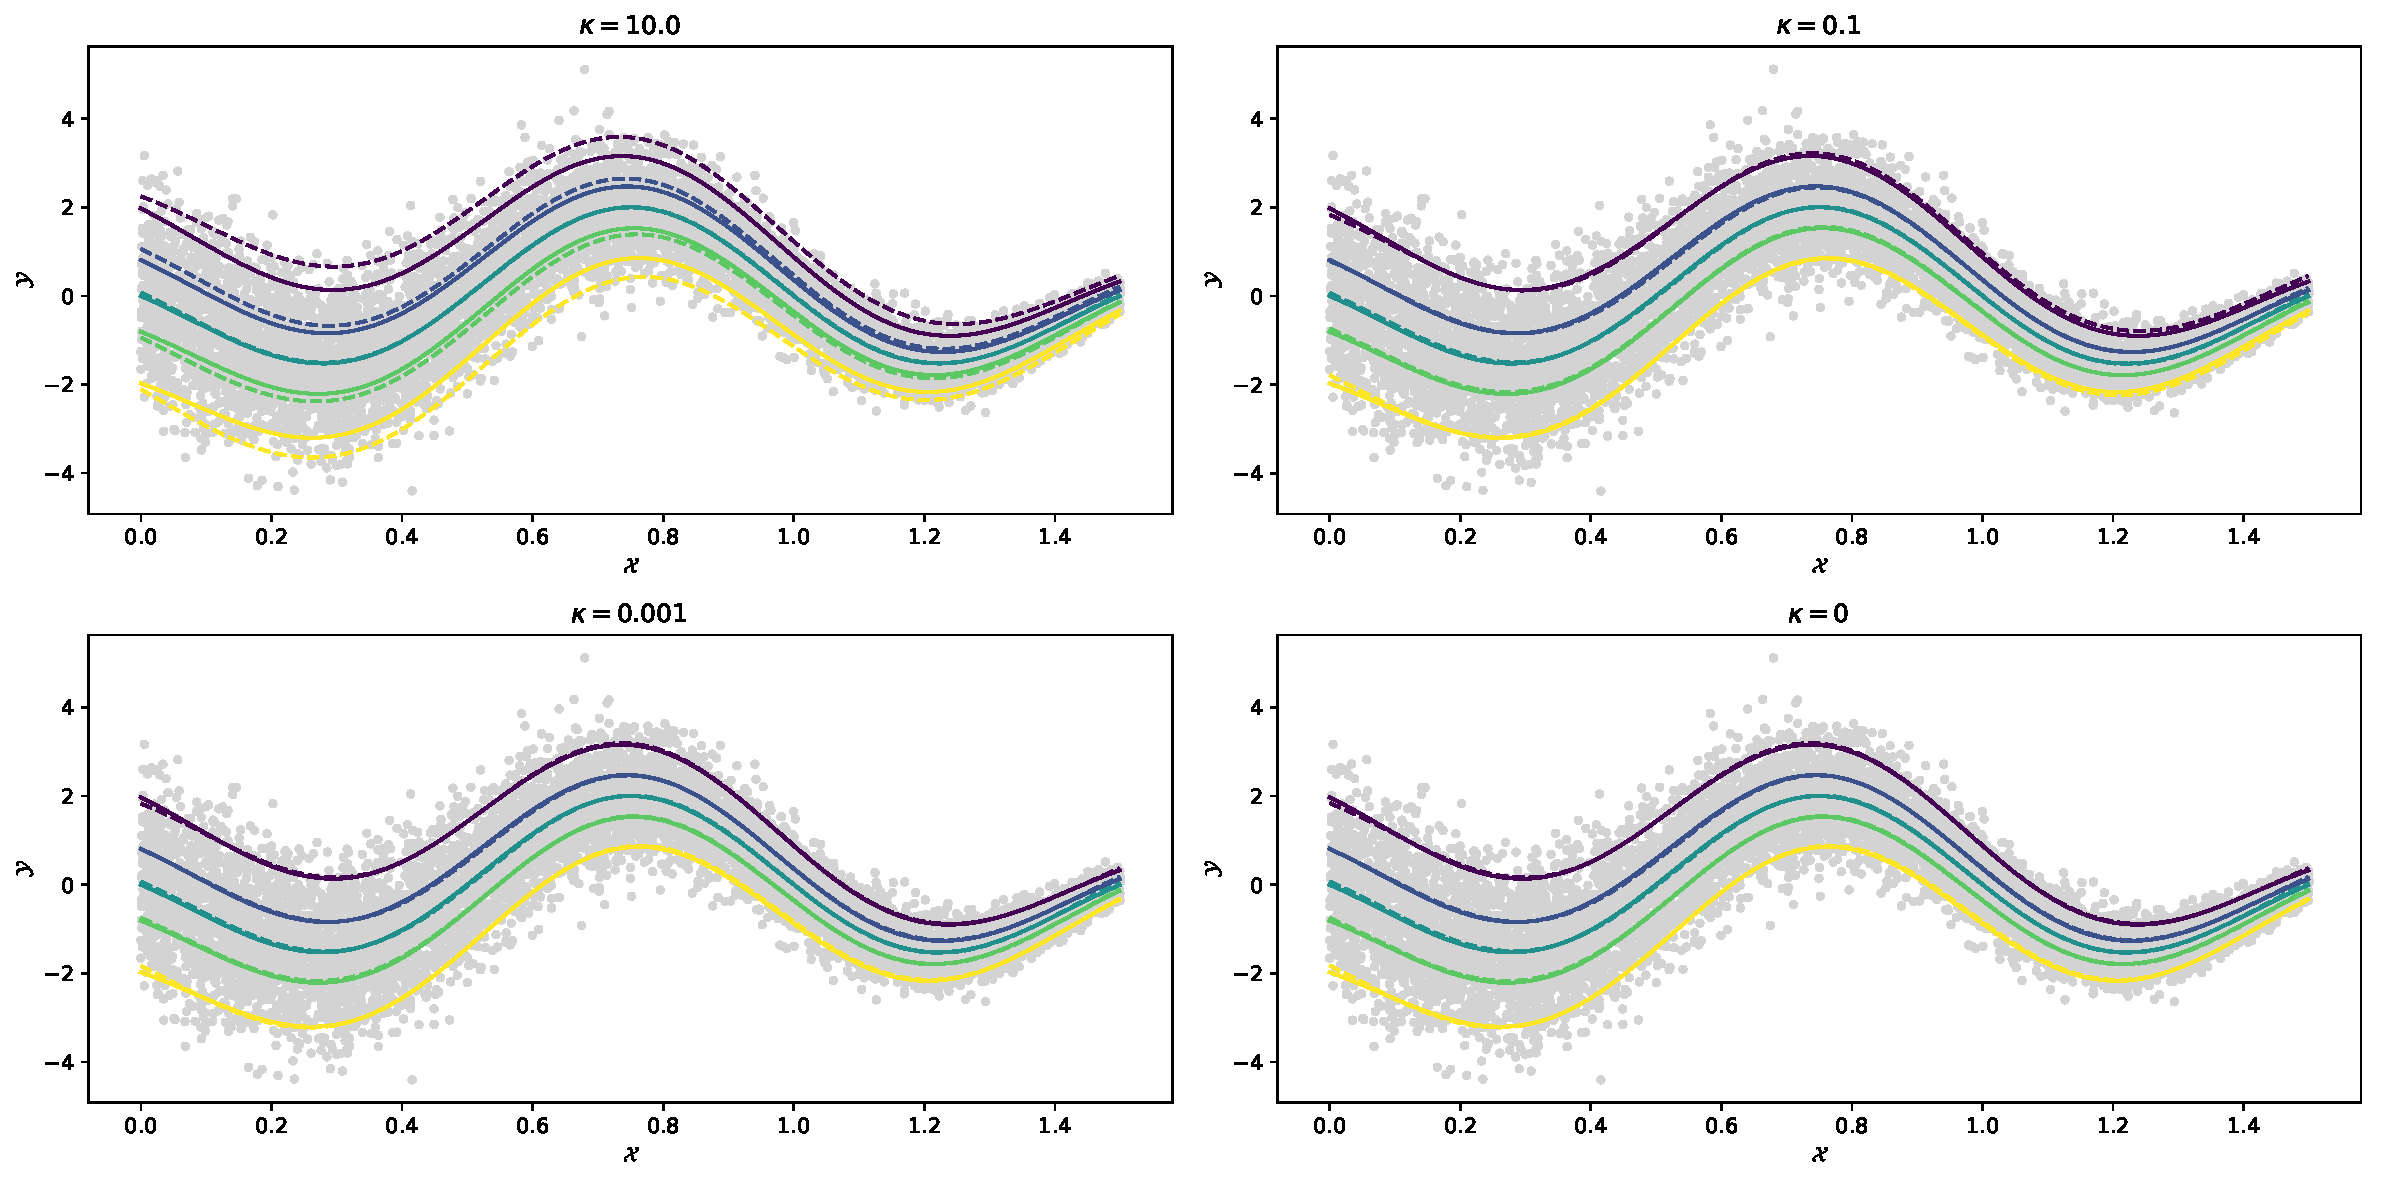
\includegraphics{src/fig/autogen/iqr_kappa.pdf}}
    \caption{Impact of the Huber loss smoothing of the pinball loss for
    differents values of $\kappa$. \label{figure:kappa_study}}
\end{figure}
\begin{table}[tb]
    \caption{Examples for objective \eqref{equation:integrated_cost}.
    $\psi_1^\kappa$, $\psi_+^\kappa$: $\kappa$-smoothed absolute value
    and positive part. $h_{x}(\hyperparameter)\defeq h(x)(\theta)$.
    \label{table:integrated_risks}}
    \begin{center}
      \addtolength{\tabcolsep}{-3pt}
      \renewcommand{\arraystretch}{0.8}
        \begin{tiny}
            \begin{sc}
                \resizebox{\textwidth}{!}{%
                \begin{tabular}{lll}
                    \toprule
                    & loss & penalty \\
                    \midrule
                    Quantile  & $\displaystyle\int_{\closedinterval{0}{1}}
                    \abs{\hyperparameter - \indicator{\reals_{-}}(y -
                    h_x(\hyperparameter))}\abs{y - h_x(\hyperparameter)}
                    d\mu(\hyperparameter)$ &
                    $\lambda_{nc}\int_{\closedinterval{0}{1}}
                    \abs{-\frac{dh_x}{d\hyperparameter}(\hyperparameter)}_+
                    d\mu(\hyperparameter) +
                    \frac{\lambda}{2}\norm{h}_{\mcH_K}^2$ \\
                    M-Quantile (smooth)  &
                    $\displaystyle\int_{\closedinterval{0}{1}}
                    \abs{\hyperparameter - \indicator{\reals_{-}}(y -
                    h_x(\hyperparameter))}\psi_1^\kappa\left(y -
                    h_x(\hyperparameter)\right)d\mu(\hyperparameter)$ &
                    $\lambda_{nc}\int_{(0, 1)} \psi_+^\kappa\left(-
                    \frac{dh_x}{d\hyperparameter}(\hyperparameter)\right)
                    d\mu(\hyperparameter) +
                    \frac{\lambda}{2}\norm{h}_{\mcH_K}^2$ \\
                    Expectiles (smooth) &
                    $\displaystyle\int_{\closedinterval{0}{1}}
                    \abs{\hyperparameter - \indicator{\reals_{-}}(y -
                    h_x(\hyperparameter))}\left(y -
                    h_x(\hyperparameter)\right)^2d\mu(\hyperparameter)$ &
                    $\lambda_{nc} \int_{(0, 1)}
                    \abs{-\frac{dh_x}{d\hyperparameter}(\hyperparameter)}_+^2
                    d\mu(\hyperparameter) +
                    \frac{\lambda}{2}\norm{h}_{\mcH_K}^2$ \\
                    Cost-Sensitive & $\displaystyle\int_{
                    \closedinterval{-1}{1}} \abs{\frac{\hyperparameter + 1}{2}
                    - \indicator{\{-1\}}(y)}\abs{1 -
                    yh_{x}(\hyperparameter)}_{+} d\mu(\theta)$ & $
                    \frac{\lambda}{2}\norm{h}_{\mcH_K}^2$ \\
                    Cost-Sensitive (smooth) &
                    $\displaystyle\int_{\closedinterval{-1}{1}}
                    \abs{\frac{\hyperparameter + 1}{2} -
                    \indicator{\{-1\}}(y)}\psi_+^\kappa\left(1 -
                    yh_{x}(\hyperparameter)\right) d\mu(\theta)$ & $
                    \frac{\lambda}{2}\norm{h}_{\mcH_K}^2$ \\
                    Level-Set   &
                    $\displaystyle\int_{\closedinterval{\epsilon}{1}}
                    -t(\hyperparameter) +
                    \frac{1}{\theta}\abs{t(\hyperparameter) -
                    h_x(\hyperparameter)}_+
                    d\mu(\hyperparameter)$ & $
                    \frac{1}{2}\displaystyle\int_{
                    \closedinterval{\epsilon}{1}}
                    \norm{h(\cdot)(\hyperparameter)}_{
                    \mcH_{k_{\inputspace}}}^2 d\mu(\hyperparameter) +
                    \frac{\lambda}{2}\norm{t}_{\mcH_{k_b}}^2$\\ \bottomrule
                \end{tabular}}
            \end{sc}
        \end{tiny}
        \addtolength{\tabcolsep}{3pt}
        \renewcommand{\arraystretch}{0.8}
    \end{center}
\end{table}
%
\subsection{Experimental protocol for \ac{QR}}  \label{subsection:proto_exp} In
this section, we give additional details regarding the choices being made while
implementing the \ac{ITL} method for $\infty$-\ac{QR}.
%
%\paragraph{Crossing Quantiles}
%The model was trained with a
%bias.  For $k_{\inputspace}$ a Gaussian kernel was used,
%$k_{\hyperparameterspace}$ and $k_{b}$ were Laplacian kernels. All bandwidths
%were set to $10$ to emphasise the possible crossings.

%\begin{dmath}\label{equation:non_crossing_constraint}
    %\Omega(h) = \lambda_{c}\sum_{i=1}^N \int_{(0, 1)} \abs{
    %-\frac{\partial}{\partial \tau} h_{\tau}(X_i)}_+ d\mu(\tau) +
    %\frac{\lambda}{2}(\norm{f}_{K}^2 + \norm{b}_{kb}^2).
%\end{dmath}
%Note that if the integral in \cref{equation:non_crossing_constraint} in uses
%the same samples $\tau_j$'s as the one used to approximate the cost function
%$\cost$, then the representer theorem applies with the expansion given in
%\cref{equation:expanded_non_crossing_constraint}.
%\begin{dmath}\label{equation:expanded_non_crossing_constraint}
    %\Omega_\lambda(h)=\lambda\sum_{j=1}^T\sum_{i=1}^N \abs{-\sum_{j'=1}^T
    %\sum_{i'=1}^N\alpha_{i'j'} k_{\inputspace}(x_i, x_{i'})\frac{\partial
    %k_{\hyperparameterspace}}{\partial\tau_j}(\tau_j, \tau_{j'}) -
    %\beta_j\frac{\partial k_b}{\partial \tau_j}(\tau_j, \tau_{j'})}_+ +
    %\sum_{i, i'=1}^N\sum_{j,
    %j'=1}^T\alpha_{ij}\alpha_{i'j'}k_{\inputspace}(x_i,
    %x_{i'})k_{\hyperparameterspace}(\tau_j,
    %\tau_{j'})+\beta_{j}\beta_{j'}k_b(\tau_j, \tau_{j'}).
%\end{dmath}
%\begin{center}
    %\begin{figure}[h]
        %% \resizebox{!}{.65\linewidth}{\includegraphics{fig/bias_experiment.eps}}
        %\caption{Model misspecification in quantile regression on the dataset
        %Engel. Left plot shows a linear model with bias and right plot without
        %bias.\label{figure:misspecified_models}}
    %\end{figure}
%\end{center}
%\par
%
\paragraph{\ac{QR} real datasets}
%
For $\infty$-\ac{QR}, $k_{\inputspace}$, $k_{\hyperparameterspace}$ were
Gaussian kernels. We set a bias term $k_b=k_{\hyperparameterspace}$. The
hyperparameters optimized were $\lambda$, the weight of the ridge penalty,
$\sigma_\inputspace$, the input kernel parameter, and
$\sigma_\hyperparameterspace=\sigma_b$, the output kernel parameter. They were
optimized in the (log)space of $\closedinterval{10^{-6}}{10^{6}}^3$. The
non-crossing constraint $\lambda_{nc}$ was set to $1$. The model was trained on
the continuum $\Theta=\openinterval{0}{1}$ using QMC and Sobol sequences. For
all datasets we draw $m=100$ quantiles form a Sobol sequence \par
%
For \ac{JQR} we similarly chose two Gaussian kernels. The optimized
hyperparameters were the same as for $\infty$-\ac{QR}.
% are also the bandwidth of the Gaussian kernel acting on the inputs, the bandwith
% of the kernel acting on the outputs, and the regularization tradeoff $\lambda$
% which where optimized in the (log)space $\closedinterval{10^{-6}}{10^{6}}^3$.
The quantiles learned were $\theta\in\Set{0.1, 0.3, 0.5, 0.7, 0.9}$.

For the IND-\ac{QR} baseline, we trained independently a non-paramatric
quantile estimator as described in \citet{takeuchi2006nonparametric}. A
Gaussian kernel was used and its bandwidth was optimized in the (log)space of
$\closedinterval{10^{-6}}{10^6}$. No non-crossing was enforced. \par
%
% \paragraph{Impact of the $\mcH_{k_{\hyperparameterspace}}$ kernel}
% See \cref{figure:gamma_t_study}.
% \begin{center}
%     \begin{figure}
%         % \resizebox{!}{.5\linewidth}{\includegraphics{fig/gamma_t_study.eps}}
%         \caption{Impact of the hyperparameter $\gamma_{\tau}$ on the
%         hyperparameter kernel $k_{\hyperparameterspace}$. Top row shows models
%         with a bias terms for $\gamma_{\tau}\in\Set{0.1, 100}$
%         respectfully left to right.  Bottom row shows the same for models
%         without bias.}
%     \label{figure:gamma_t_study}
%     \end{figure}
% \end{center}
\subsection{Experiments with \ac{CSC}}
\label{subsection:csc_expe}
In this section we provide numerical illustration concerning the \ac{CSC} problem.
We used the Iris \acs{UCI} dataset with $4$ attributes and $150$
samples, the two synthetic \textsc{scikit-learn}
\citep{pedregosa2011scikit} datasets \textsc{Two-Moons} (noise=$0.4$) and
$\textsc{Circles}$ (noise=$0.1$) with both $2$ attributes and $1000$
samples and a third synthetic \textsc{scikit-learn} dataset \textsc{Toy}
(class sep=$0.5$) with $20$ features ($4$ redundant and $10$ informative)
and $n=1000$ samples.\par
%
As detailed in \cref{section:infinite_tasks}, \acl{CSC} on a continuum
$\hyperparameterspace = \closedinterval{-1}{1}$ that we call \ac{ICSC}
can be tackled by our proposed technique.  In this case, the hyperparameter
$\hyperparameter$ controls the tradeoff between the importance of the correct
classification with labels $-1$ and $+1$. When $\hyperparameter = -1$,
class $-1$ is emphasized; the probability of correctly classified instances
with this label (called specificity) is desired to be $1$.  Similarly, for
$\hyperparameter = +1$, the probability of correct classification of samples
with label $+1$ (called sensitivity) is ideally $1$.\par
%
To illustrate the advantage of (infinite) joint learning we used two synthetic
datasets \textsc{Circles} and \textsc{Two-Moons} and the \acs{UCI}
\textsc{Iris} dataset. We chose $k_{\inputspace}$ to be a Gaussian kernel with
bandwidth $\sigma_{\inputspace}=(2\gamma_{\inputspace})^{(-1/2)}$ the median of
the Euclidean pairwise distances of the input points \citep{jaakkola1999using}.
$k_{\hyperparameterspace}$ is also a Gaussian kernel with bandwidth
$\gamma_{\hyperparameterspace}=5$.  We used $m=20$ for all datasets.
%
As a baseline we trained independently 3 \acl{CSC} classifiers with
$\hyperparameter\in\Set{-0.9,0, 0.9}$. We repeated $50$ times a random $50-50\%$
train-test split of the dataset and report the average test error and standard
deviation (in terms of sensitivity and specificity) \par
%
Our results are illustrated in \cref{table:csc_results}. For $\theta=-0.9$, both
 independent and joint learners give the desired $100\%$ specificity; the
joint \acl{CSC} scheme however has significantly higher sensitivity value
($15\%$ vs $0\%$) on the dataset \textsc{Circles}. Similar conclusion holds for the
$\theta=+0.9$ extreme: the ideal sensitivity is reached by both techniques, but
the joint learning scheme performs better in terms of specificity ($0\%$ vs
$12\%$) on the dataset \textsc{Circles}. \par
%
\begin{table*}[!htbp]
    \caption{\acs{ICSC} vs Independent (IND)-\acs{CSC}. Higher is
    better.\label{table:csc_results}}
    \addtolength{\tabcolsep}{-3pt}
    \renewcommand{\arraystretch}{0.8}% Tighter
    \begin{center}
        \begin{tiny}
            \begin{sc}
                \resizebox{.7\textwidth}{!}{%
                \begin{tabular}{cccccccc}
                    \toprule
                    \multirow{2}{*}{Dataset} & \multirow{2}{*}{Method} &
                    \multicolumn{2}{c}{$\theta=-0.9$} &
                    \multicolumn{2}{c}{$\theta=0$} &
                    \multicolumn{2}{c}{$\theta=+0.9$} \\
                    \cmidrule(lr){3-4} \cmidrule(lr){5-6} \cmidrule(lr){7-8} &
                    & \textsc{sensitivity} & \textsc{specificity} &
                    \textsc{sensitivity} & \textsc{specificity} &
                    \textsc{sensitivity} & \textsc{specificity} \\
                    \midrule
                    \multirow{ 2}{*}{\textsc{Two-Moons}} & IND &
                    $0.3\pm0.05$ & $0.99\pm0.01$ & $0.83\pm0.03$ &
                    $0.86\pm0.03$ & $0.99\pm0$ & $0.32\pm0.06$ \\
                                                & \acs{ICSC} & $0.32\pm0.05$ &
                    $0.99\pm0.01$ & $0.84\pm0.03$ & $0.87\pm0.03$ & $1\pm0$ &
                    $0.36\pm0.04$  \\
                    \multirow{ 2}{*}{\textsc{Circles}} & IND & $0\pm0$
                    & $1\pm0$ & $0.82\pm0.02$ & $0.84\pm0.03$ & $1\pm0$ &
                    $0\pm0$ \\
                                              & \acs{ICSC} & $0.15\pm0.05$ &
                    $1\pm0$ & $0.82\pm0.02$ & $0.84\pm0.03$ & $1\pm0$ &
                    $0.12\pm0.05$  \\
                    \multirow{ 2}{*}{\textsc{Iris}} & IND &
                    $0.88\pm0.08$ & $ 0.94\pm0.06$ & $0.94\pm0.05$ &
                    $0.92\pm0.06$ & $0.97\pm0.05$ & $0.87\pm0.06$\\
                                           & \acs{ICSC} & $0.89\pm0.08$ &
                    $0.94\pm0.05$ & $0.94\pm0.06$ & $0.92\pm0.05$ &
                    $0.97\pm0.04$ & $0.90\pm0.05$
                    \\
                    \multirow{ 2}{*}{\textsc{Toy}} & IND &
                    $0.51\pm0.06$ & $ 0.98\pm0.01$ & $0.83\pm0.03$ &
                    $0.86\pm0.03$ & $0.97\pm0.01$ & $0.49\pm0.07$\\
                                           & \acs{ICSC} & $0.63\pm0.04$ &
                    $0.96\pm0.01$ & $0.83\pm0.03$ & $0.85\pm0.03$ &
                    $0.95\pm0.02$ & $0.61\pm0.04$
                    \\
                    \bottomrule
                \end{tabular}}
            \end{sc}
        \end{tiny}
    \end{center}
    \addtolength{\tabcolsep}{3pt}
    \renewcommand{\arraystretch}{1.0}% Tighter
\end{table*}
% \subsubsection{Illustration of the \ac{CSC} datasets}
% \begin{figure}[!htbp]
% \setlength\fboxsep{0pt}\setlength\fboxrule{0.75pt}
% \ffigbox[\textwidth]
% {
% \begin{subfloatrow}[2]
% %\fbox{
% \ffigbox[.49\textwidth]
%   {
%     \caption{\textsc{Circle} dataset}
%     \label{subfigure:csc_circle}
%   }
%   {
%     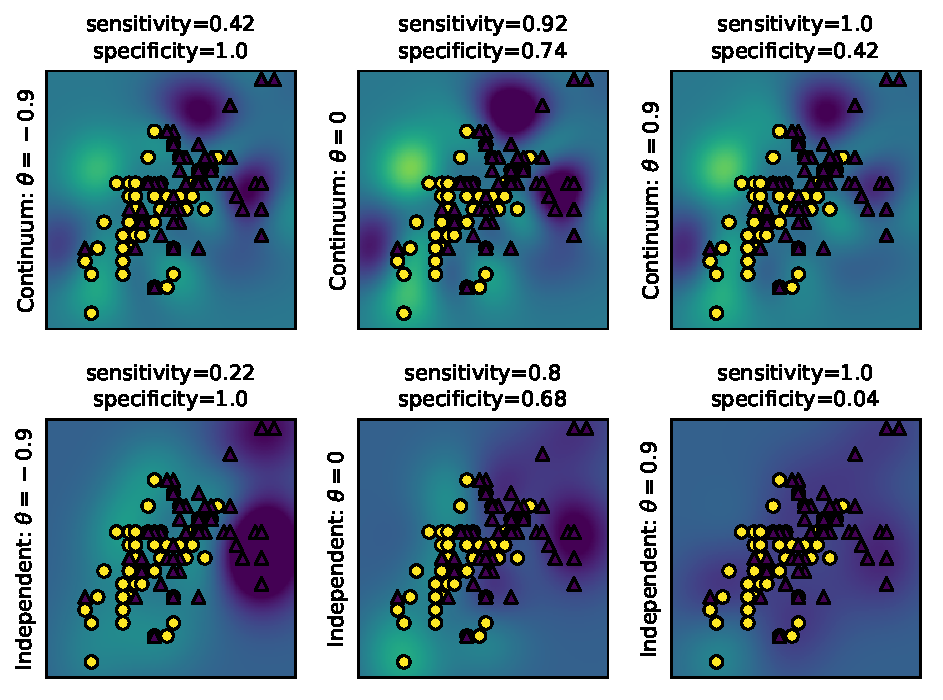
\includegraphics[angle=-90,width=\linewidth]{src/fig/autogen/icsl_vs.pdf}%
%   }
% %}
% %\fbox{
% \ffigbox[.4825\textwidth]
%   {
%     \caption{\textsc{Two-Moons} dataset}
%     \label{subfigure:csc_moons}
%   }
%   {
%     \includegraphics[angle=-90,width=\linewidth]{src/fig/autogen/icsl_vs_moons.pdf}%
%   }
% %}
% \end{subfloatrow}%
% }
% {
%     \caption{Illustration of some datasets used in \cref{table:csc_results}.
%     \label{figure:csc_datasets}}
% }
% \end{figure}%
% \textsc{Two-Moons} and \textsc{Circles} used in \cref{table:csc_results}.

\printbibliography[heading=subbibliography]
\end{refsection}
%\ifthenelse{\NOT\isundefined{\draft}\OR\NOT\isundefined{\final}}{
    %\subsubsection*{Acronyms}
    %\printacronyms[heading=none]
%}{}
%

%\section{Additional Experiments}
%We present here more details on the experimental protocol used in the main
paper as well as new experiments.
\subsection{Alternative hyperparameters sampling}\label{subsection:sampling}
Many quadrature rules such as \ac{MC} and \ac{QMC} methods are well suited for
\acl{ITL}. For instance when $\hyperparameterspace$ is high dimensional,
\ac{MC} is typically prefered over \ac{QMC}, and vice versa. If
$\hyperparameterspace$ is one dimensional and the function to integrate is
smooth enough then a Gauss-Legendre quadrature would be preferable. In
\cref{sec:V} of the main paper we provide a unified notation to handle
\ac{MC}, \ac{QMC} and other quadrature rules. In the case of
\begin{itemize}
    \item \ac{MC}: $w_j = \frac{1}{m}$ and $(\theta_j)_{j=1}^m
    \sim \mu^{\otimes m}$.
    %Note that if $\mu=\delta_{\theta_j'}$ is a dirac measure  centered at
    %$\theta_{j'}$ then $\theta_j=\theta_j'$.
    \item \ac{QMC}: $w_j = m^{-1}F^{-1}(\theta_j)$ and $(\theta_j)_{j=1}^m$
    is a sequence with values in $[0, 1]^d$ such as the % uniform properties
    Sobol or Halton sequence, $\mu$ is assumed to be absolutely continuous
    \acs{wrt} the Lebesgue measure, $F$ is the associated cdf.
    \item Quadrature rules: $((\theta_j, w'_j))_{j=1}^m$ is the indexed set of
    locations and weights produced by the quadrature rule, $w_j
    = w'_j f_{\mu}(\theta_j)$, $\mu$ is assumed to be absolutely continuous
    \acs{wrt} the Lebesgue measure, and $f_\mu$ denotes its corresponding
    probability density function.
\end{itemize}
\subsection{Impact of the number of hyperparameters sampled}
\begin{figure}[!htbp]
    \centering
    \includegraphics[width=\textwidth]{src/fig/autogen/iqr_m.pdf}
    \caption{Impact of the number of hyperparameters sampled.
             \label{figure:iqr_m}}
\end{figure}
In the experiment presented on \cref{figure:iqr_m}, on the sine synthetic
benchmark, we draw $n=1000$ training points and study the impact of increasing
$m$ on the quality of the quantiles at $\theta\in\Set{0.05, 0.25, 0.5, 0.75,
0.95}$. We notice that when $m\ge34\approx\sqrt{1000}$ there is little benefit
to draw more $m$ samples are the quantile curves do not change on the
$n_{\text{test}}=2000$ test points.
\subsection{Smoothifying the cost function} \label{subsection:infimal_convo}
The resulting $\kappa$-smoothed ($\kappa\in\reals_+$) absolute value
($\psi_{1}^\kappa$) and positive part ($\psi_{+}^\kappa$) are as follows:
\begin{align*}
  \psi_{1}^\kappa(p) &\defeq \left(\kappa \abs{\cdot} \square \frac{1}{2}
    \abs{\cdot}^2 \right)(p)
     =
     \begin{cases}
        \frac{1}{2\kappa}p^2 & \text{if $\abs{p} \le \kappa$} \\
        \abs{p} - \frac{\kappa}{2} & \text{otherwise},
    \end{cases}\\
     \psi_{+}^\kappa(p) &\defeq \left(\kappa\abs{\cdot}_+ \square\frac{1}{2}
     \abs{\cdot}^2 \right)(p) =
     \begin{cases}
         \frac{1}{2\kappa}\abs{p}_+^2 & \text{if $p \le \kappa$} \\
         p - \frac{\kappa}{2} & \text{otherwise.}
     \end{cases}
\end{align*}
where $\square$ is the classical infimal convolution \citep{bauschke2011convex}.
All the smoothified loss functions used in this paper
have been gathered in \cref{table:integrated_risks}.
\paragraph{Remarks}
\begin{itemize}[labelindent=0cm,leftmargin=*,topsep=0cm,partopsep=0cm,
                parsep=0cm,itemsep=0cm]
    \item Minimizing the $\kappa$-smoothed pinball loss
    \begin{align*}
     \parametrizedcost{\hyperparameter,\kappa}(y, h(x))=\abs{\hyperparameter -
     \indicator{\reals_{-}}(y - h(x))}\psi_1^\kappa(y - h(x)),
    \end{align*}
    yields the quantiles when $\kappa\rightarrow 0$, the expectiles as
    $\kappa\to+\infty$. The intermediate values are known as M-quantiles
    \citep{breckling1988m}.
    \item In practice, the absolute value and positive part can be approximated
    by a smooth function by setting the smoothing parameter $\kappa$ to be a
    small positive value;
    % \rb{or even zero}
    the optimization showed a robust behaviour \acs{wrt} this choice with a
    random coefficient initialization.
    % \rb{as    pointed out by \citet{lewis2013nonsmooth}}.
%     \item the cost of evaluating the model $h$ one $n$ samples and $m$
%     hyperparameters is $\mathcal{O}(n^2m + m^2n)$ and it takes
%     $\mathcal{O}(m^2+n^2)$ to fit in memory.
\end{itemize}\par
\paragraph{Impact of the Huber loss support}
The influence of the $\kappa$ parameter is illustrated in
\cref{figure:kappa_study}.  For this experiment, $10000$ samples have been
generated from the sine wave dataset described in \cref{paragraph:datasets},
and the model have been trained on $100$ quantiles generated from a
Gauss-Legendre Quadrature.  When $\kappa$ is large the expectiles are learnt
(dashed lines) while when $\kappa$ is small the quantiles are recovered (the
dashed lines on the right plot match the theoretical quantiles in plain lines).
It took $225$s ($258$ iteration, and $289$ function evaluations) to train
for $\kappa=1\cdot 10^1$, $1313$s for $\kappa=1\cdot 10^{-1}$ ($1438$
iterations and $1571$ function evaluations), $931$s for $\kappa=1e^{-3}$
($1169$ iterations and $1271$ function evaluations) and $879$s for $\kappa=0$
($1125$ iterations and $1207$ function evaluations). We used a GPU Tensorflow
implementation and run the experiments in float64 on a computer equipped with a
GTX $1070$, and intel i7 $7700$ and $16$GB of DRAM.
\begin{figure}[!htbp]
    \centering
    \resizebox{!}{.5\linewidth}{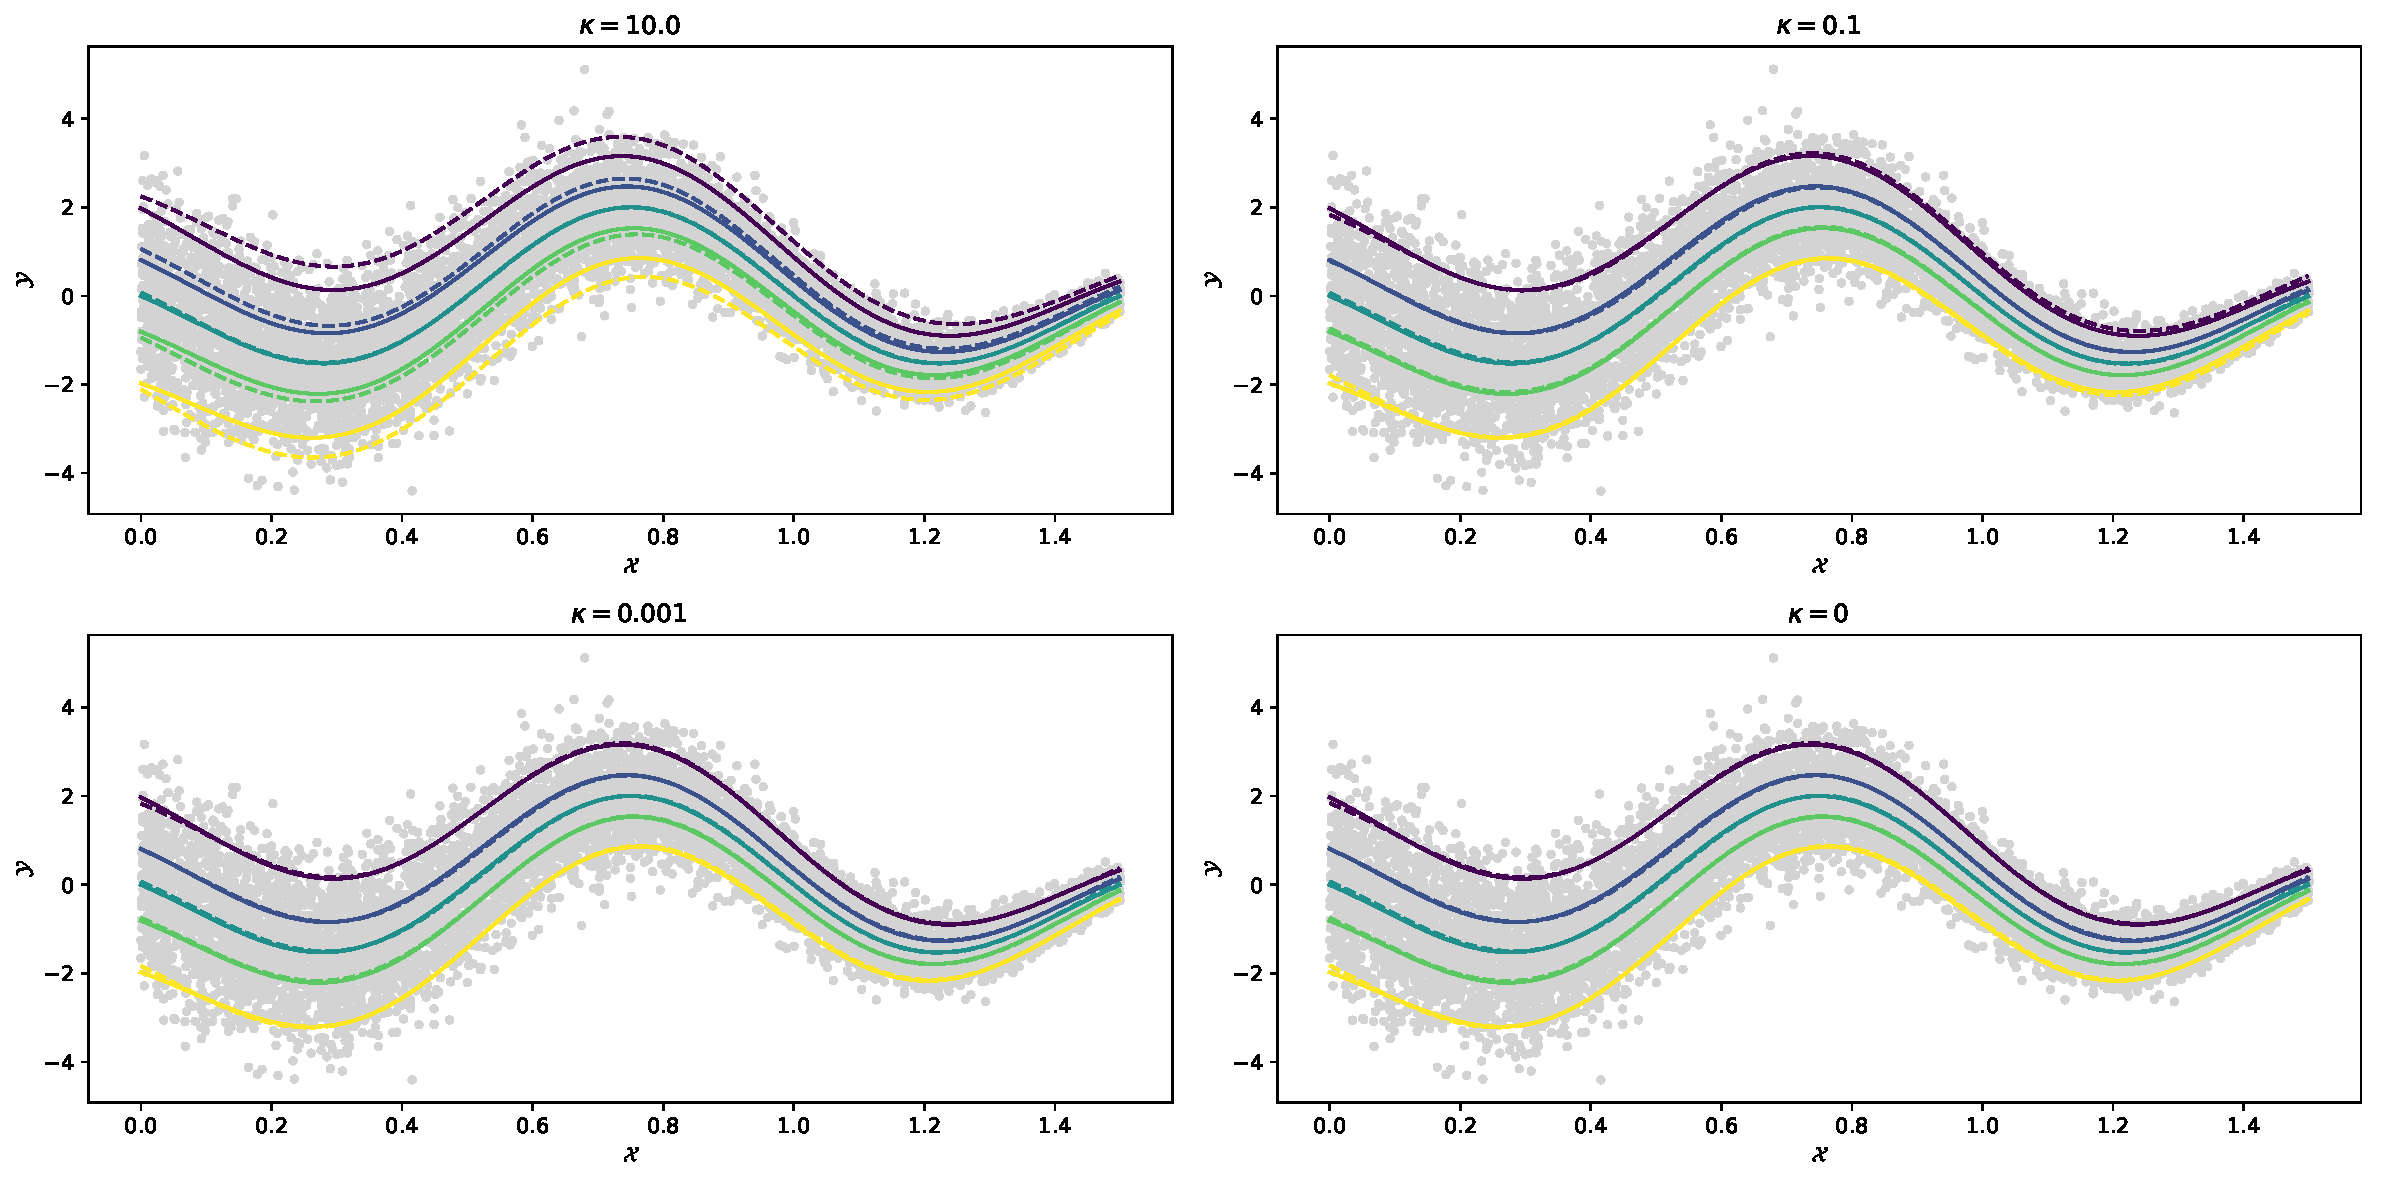
\includegraphics{src/fig/autogen/iqr_kappa.pdf}}
    \caption{Impact of the Huber loss smoothing of the pinball loss for
    differents values of $\kappa$. \label{figure:kappa_study}}
\end{figure}
\begin{table}[tb]
    \caption{Examples for objective \eqref{equation:integrated_cost}.
    $\psi_1^\kappa$, $\psi_+^\kappa$: $\kappa$-smoothed absolute value
    and positive part. $h_{x}(\hyperparameter)\defeq h(x)(\theta)$.
    \label{table:integrated_risks}}
    \begin{center}
      \addtolength{\tabcolsep}{-3pt}
      \renewcommand{\arraystretch}{0.8}
        \begin{tiny}
            \begin{sc}
                \resizebox{\textwidth}{!}{%
                \begin{tabular}{lll}
                    \toprule
                    & loss & penalty \\
                    \midrule
                    Quantile  & $\displaystyle\int_{\closedinterval{0}{1}}
                    \abs{\hyperparameter - \indicator{\reals_{-}}(y -
                    h_x(\hyperparameter))}\abs{y - h_x(\hyperparameter)}
                    d\mu(\hyperparameter)$ &
                    $\lambda_{nc}\int_{\closedinterval{0}{1}}
                    \abs{-\frac{dh_x}{d\hyperparameter}(\hyperparameter)}_+
                    d\mu(\hyperparameter) +
                    \frac{\lambda}{2}\norm{h}_{\mcH_K}^2$ \\
                    M-Quantile (smooth)  &
                    $\displaystyle\int_{\closedinterval{0}{1}}
                    \abs{\hyperparameter - \indicator{\reals_{-}}(y -
                    h_x(\hyperparameter))}\psi_1^\kappa\left(y -
                    h_x(\hyperparameter)\right)d\mu(\hyperparameter)$ &
                    $\lambda_{nc}\int_{(0, 1)} \psi_+^\kappa\left(-
                    \frac{dh_x}{d\hyperparameter}(\hyperparameter)\right)
                    d\mu(\hyperparameter) +
                    \frac{\lambda}{2}\norm{h}_{\mcH_K}^2$ \\
                    Expectiles (smooth) &
                    $\displaystyle\int_{\closedinterval{0}{1}}
                    \abs{\hyperparameter - \indicator{\reals_{-}}(y -
                    h_x(\hyperparameter))}\left(y -
                    h_x(\hyperparameter)\right)^2d\mu(\hyperparameter)$ &
                    $\lambda_{nc} \int_{(0, 1)}
                    \abs{-\frac{dh_x}{d\hyperparameter}(\hyperparameter)}_+^2
                    d\mu(\hyperparameter) +
                    \frac{\lambda}{2}\norm{h}_{\mcH_K}^2$ \\
                    Cost-Sensitive & $\displaystyle\int_{
                    \closedinterval{-1}{1}} \abs{\frac{\hyperparameter + 1}{2}
                    - \indicator{\{-1\}}(y)}\abs{1 -
                    yh_{x}(\hyperparameter)}_{+} d\mu(\theta)$ & $
                    \frac{\lambda}{2}\norm{h}_{\mcH_K}^2$ \\
                    Cost-Sensitive (smooth) &
                    $\displaystyle\int_{\closedinterval{-1}{1}}
                    \abs{\frac{\hyperparameter + 1}{2} -
                    \indicator{\{-1\}}(y)}\psi_+^\kappa\left(1 -
                    yh_{x}(\hyperparameter)\right) d\mu(\theta)$ & $
                    \frac{\lambda}{2}\norm{h}_{\mcH_K}^2$ \\
                    Level-Set   &
                    $\displaystyle\int_{\closedinterval{\epsilon}{1}}
                    -t(\hyperparameter) +
                    \frac{1}{\theta}\abs{t(\hyperparameter) -
                    h_x(\hyperparameter)}_+
                    d\mu(\hyperparameter)$ & $
                    \frac{1}{2}\displaystyle\int_{
                    \closedinterval{\epsilon}{1}}
                    \norm{h(\cdot)(\hyperparameter)}_{
                    \mcH_{k_{\inputspace}}}^2 d\mu(\hyperparameter) +
                    \frac{\lambda}{2}\norm{t}_{\mcH_{k_b}}^2$\\ \bottomrule
                \end{tabular}}
            \end{sc}
        \end{tiny}
        \addtolength{\tabcolsep}{3pt}
        \renewcommand{\arraystretch}{0.8}
    \end{center}
\end{table}
%
\subsection{Experimental protocol for \ac{QR}}  \label{subsection:proto_exp} In
this section, we give additional details regarding the choices being made while
implementing the \ac{ITL} method for $\infty$-\ac{QR}.
%
%\paragraph{Crossing Quantiles}
%The model was trained with a
%bias.  For $k_{\inputspace}$ a Gaussian kernel was used,
%$k_{\hyperparameterspace}$ and $k_{b}$ were Laplacian kernels. All bandwidths
%were set to $10$ to emphasise the possible crossings.

%\begin{dmath}\label{equation:non_crossing_constraint}
    %\Omega(h) = \lambda_{c}\sum_{i=1}^N \int_{(0, 1)} \abs{
    %-\frac{\partial}{\partial \tau} h_{\tau}(X_i)}_+ d\mu(\tau) +
    %\frac{\lambda}{2}(\norm{f}_{K}^2 + \norm{b}_{kb}^2).
%\end{dmath}
%Note that if the integral in \cref{equation:non_crossing_constraint} in uses
%the same samples $\tau_j$'s as the one used to approximate the cost function
%$\cost$, then the representer theorem applies with the expansion given in
%\cref{equation:expanded_non_crossing_constraint}.
%\begin{dmath}\label{equation:expanded_non_crossing_constraint}
    %\Omega_\lambda(h)=\lambda\sum_{j=1}^T\sum_{i=1}^N \abs{-\sum_{j'=1}^T
    %\sum_{i'=1}^N\alpha_{i'j'} k_{\inputspace}(x_i, x_{i'})\frac{\partial
    %k_{\hyperparameterspace}}{\partial\tau_j}(\tau_j, \tau_{j'}) -
    %\beta_j\frac{\partial k_b}{\partial \tau_j}(\tau_j, \tau_{j'})}_+ +
    %\sum_{i, i'=1}^N\sum_{j,
    %j'=1}^T\alpha_{ij}\alpha_{i'j'}k_{\inputspace}(x_i,
    %x_{i'})k_{\hyperparameterspace}(\tau_j,
    %\tau_{j'})+\beta_{j}\beta_{j'}k_b(\tau_j, \tau_{j'}).
%\end{dmath}
%\begin{center}
    %\begin{figure}[h]
        %% \resizebox{!}{.65\linewidth}{\includegraphics{fig/bias_experiment.eps}}
        %\caption{Model misspecification in quantile regression on the dataset
        %Engel. Left plot shows a linear model with bias and right plot without
        %bias.\label{figure:misspecified_models}}
    %\end{figure}
%\end{center}
%\par
%
\paragraph{\ac{QR} real datasets}
%
For $\infty$-\ac{QR}, $k_{\inputspace}$, $k_{\hyperparameterspace}$ were
Gaussian kernels. We set a bias term $k_b=k_{\hyperparameterspace}$. The
hyperparameters optimized were $\lambda$, the weight of the ridge penalty,
$\sigma_\inputspace$, the input kernel parameter, and
$\sigma_\hyperparameterspace=\sigma_b$, the output kernel parameter. They were
optimized in the (log)space of $\closedinterval{10^{-6}}{10^{6}}^3$. The
non-crossing constraint $\lambda_{nc}$ was set to $1$. The model was trained on
the continuum $\Theta=\openinterval{0}{1}$ using QMC and Sobol sequences. For
all datasets we draw $m=100$ quantiles form a Sobol sequence \par
%
For \ac{JQR} we similarly chose two Gaussian kernels. The optimized
hyperparameters were the same as for $\infty$-\ac{QR}.
% are also the bandwidth of the Gaussian kernel acting on the inputs, the bandwith
% of the kernel acting on the outputs, and the regularization tradeoff $\lambda$
% which where optimized in the (log)space $\closedinterval{10^{-6}}{10^{6}}^3$.
The quantiles learned were $\theta\in\Set{0.1, 0.3, 0.5, 0.7, 0.9}$.

For the IND-\ac{QR} baseline, we trained independently a non-paramatric
quantile estimator as described in \citet{takeuchi2006nonparametric}. A
Gaussian kernel was used and its bandwidth was optimized in the (log)space of
$\closedinterval{10^{-6}}{10^6}$. No non-crossing was enforced. \par
%
% \paragraph{Impact of the $\mcH_{k_{\hyperparameterspace}}$ kernel}
% See \cref{figure:gamma_t_study}.
% \begin{center}
%     \begin{figure}
%         % \resizebox{!}{.5\linewidth}{\includegraphics{fig/gamma_t_study.eps}}
%         \caption{Impact of the hyperparameter $\gamma_{\tau}$ on the
%         hyperparameter kernel $k_{\hyperparameterspace}$. Top row shows models
%         with a bias terms for $\gamma_{\tau}\in\Set{0.1, 100}$
%         respectfully left to right.  Bottom row shows the same for models
%         without bias.}
%     \label{figure:gamma_t_study}
%     \end{figure}
% \end{center}
\subsection{Experiments with \ac{CSC}}
\label{subsection:csc_expe}
In this section we provide numerical illustration concerning the \ac{CSC} problem.
We used the Iris \acs{UCI} dataset with $4$ attributes and $150$
samples, the two synthetic \textsc{scikit-learn}
\citep{pedregosa2011scikit} datasets \textsc{Two-Moons} (noise=$0.4$) and
$\textsc{Circles}$ (noise=$0.1$) with both $2$ attributes and $1000$
samples and a third synthetic \textsc{scikit-learn} dataset \textsc{Toy}
(class sep=$0.5$) with $20$ features ($4$ redundant and $10$ informative)
and $n=1000$ samples.\par
%
As detailed in \cref{section:infinite_tasks}, \acl{CSC} on a continuum
$\hyperparameterspace = \closedinterval{-1}{1}$ that we call \ac{ICSC}
can be tackled by our proposed technique.  In this case, the hyperparameter
$\hyperparameter$ controls the tradeoff between the importance of the correct
classification with labels $-1$ and $+1$. When $\hyperparameter = -1$,
class $-1$ is emphasized; the probability of correctly classified instances
with this label (called specificity) is desired to be $1$.  Similarly, for
$\hyperparameter = +1$, the probability of correct classification of samples
with label $+1$ (called sensitivity) is ideally $1$.\par
%
To illustrate the advantage of (infinite) joint learning we used two synthetic
datasets \textsc{Circles} and \textsc{Two-Moons} and the \acs{UCI}
\textsc{Iris} dataset. We chose $k_{\inputspace}$ to be a Gaussian kernel with
bandwidth $\sigma_{\inputspace}=(2\gamma_{\inputspace})^{(-1/2)}$ the median of
the Euclidean pairwise distances of the input points \citep{jaakkola1999using}.
$k_{\hyperparameterspace}$ is also a Gaussian kernel with bandwidth
$\gamma_{\hyperparameterspace}=5$.  We used $m=20$ for all datasets.
%
As a baseline we trained independently 3 \acl{CSC} classifiers with
$\hyperparameter\in\Set{-0.9,0, 0.9}$. We repeated $50$ times a random $50-50\%$
train-test split of the dataset and report the average test error and standard
deviation (in terms of sensitivity and specificity) \par
%
Our results are illustrated in \cref{table:csc_results}. For $\theta=-0.9$, both
 independent and joint learners give the desired $100\%$ specificity; the
joint \acl{CSC} scheme however has significantly higher sensitivity value
($15\%$ vs $0\%$) on the dataset \textsc{Circles}. Similar conclusion holds for the
$\theta=+0.9$ extreme: the ideal sensitivity is reached by both techniques, but
the joint learning scheme performs better in terms of specificity ($0\%$ vs
$12\%$) on the dataset \textsc{Circles}. \par
%
\begin{table*}[!htbp]
    \caption{\acs{ICSC} vs Independent (IND)-\acs{CSC}. Higher is
    better.\label{table:csc_results}}
    \addtolength{\tabcolsep}{-3pt}
    \renewcommand{\arraystretch}{0.8}% Tighter
    \begin{center}
        \begin{tiny}
            \begin{sc}
                \resizebox{.7\textwidth}{!}{%
                \begin{tabular}{cccccccc}
                    \toprule
                    \multirow{2}{*}{Dataset} & \multirow{2}{*}{Method} &
                    \multicolumn{2}{c}{$\theta=-0.9$} &
                    \multicolumn{2}{c}{$\theta=0$} &
                    \multicolumn{2}{c}{$\theta=+0.9$} \\
                    \cmidrule(lr){3-4} \cmidrule(lr){5-6} \cmidrule(lr){7-8} &
                    & \textsc{sensitivity} & \textsc{specificity} &
                    \textsc{sensitivity} & \textsc{specificity} &
                    \textsc{sensitivity} & \textsc{specificity} \\
                    \midrule
                    \multirow{ 2}{*}{\textsc{Two-Moons}} & IND &
                    $0.3\pm0.05$ & $0.99\pm0.01$ & $0.83\pm0.03$ &
                    $0.86\pm0.03$ & $0.99\pm0$ & $0.32\pm0.06$ \\
                                                & \acs{ICSC} & $0.32\pm0.05$ &
                    $0.99\pm0.01$ & $0.84\pm0.03$ & $0.87\pm0.03$ & $1\pm0$ &
                    $0.36\pm0.04$  \\
                    \multirow{ 2}{*}{\textsc{Circles}} & IND & $0\pm0$
                    & $1\pm0$ & $0.82\pm0.02$ & $0.84\pm0.03$ & $1\pm0$ &
                    $0\pm0$ \\
                                              & \acs{ICSC} & $0.15\pm0.05$ &
                    $1\pm0$ & $0.82\pm0.02$ & $0.84\pm0.03$ & $1\pm0$ &
                    $0.12\pm0.05$  \\
                    \multirow{ 2}{*}{\textsc{Iris}} & IND &
                    $0.88\pm0.08$ & $ 0.94\pm0.06$ & $0.94\pm0.05$ &
                    $0.92\pm0.06$ & $0.97\pm0.05$ & $0.87\pm0.06$\\
                                           & \acs{ICSC} & $0.89\pm0.08$ &
                    $0.94\pm0.05$ & $0.94\pm0.06$ & $0.92\pm0.05$ &
                    $0.97\pm0.04$ & $0.90\pm0.05$
                    \\
                    \multirow{ 2}{*}{\textsc{Toy}} & IND &
                    $0.51\pm0.06$ & $ 0.98\pm0.01$ & $0.83\pm0.03$ &
                    $0.86\pm0.03$ & $0.97\pm0.01$ & $0.49\pm0.07$\\
                                           & \acs{ICSC} & $0.63\pm0.04$ &
                    $0.96\pm0.01$ & $0.83\pm0.03$ & $0.85\pm0.03$ &
                    $0.95\pm0.02$ & $0.61\pm0.04$
                    \\
                    \bottomrule
                \end{tabular}}
            \end{sc}
        \end{tiny}
    \end{center}
    \addtolength{\tabcolsep}{3pt}
    \renewcommand{\arraystretch}{1.0}% Tighter
\end{table*}
% \subsubsection{Illustration of the \ac{CSC} datasets}
% \begin{figure}[!htbp]
% \setlength\fboxsep{0pt}\setlength\fboxrule{0.75pt}
% \ffigbox[\textwidth]
% {
% \begin{subfloatrow}[2]
% %\fbox{
% \ffigbox[.49\textwidth]
%   {
%     \caption{\textsc{Circle} dataset}
%     \label{subfigure:csc_circle}
%   }
%   {
%     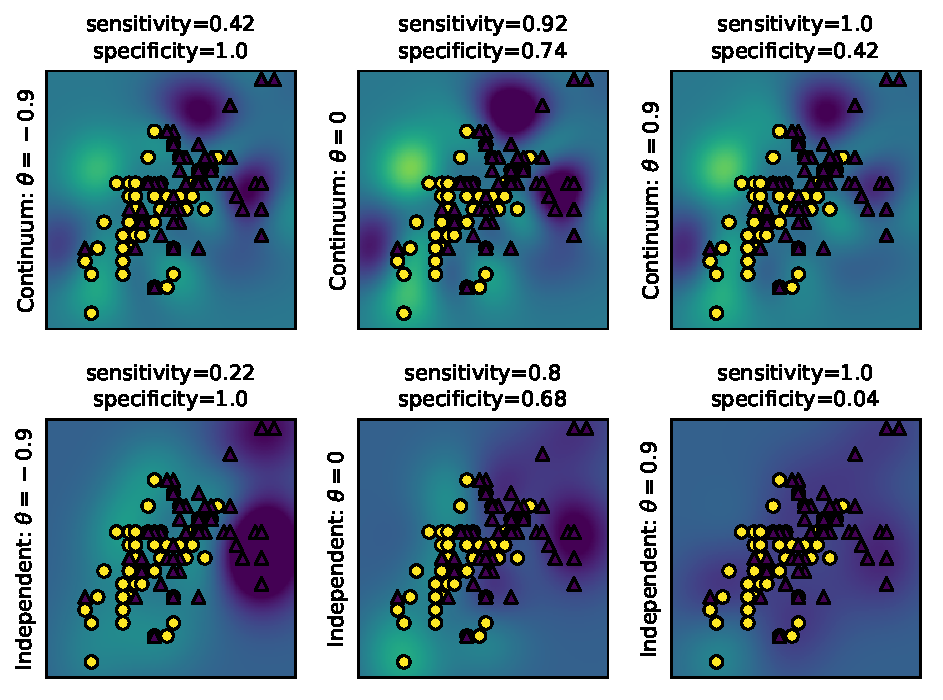
\includegraphics[angle=-90,width=\linewidth]{src/fig/autogen/icsl_vs.pdf}%
%   }
% %}
% %\fbox{
% \ffigbox[.4825\textwidth]
%   {
%     \caption{\textsc{Two-Moons} dataset}
%     \label{subfigure:csc_moons}
%   }
%   {
%     \includegraphics[angle=-90,width=\linewidth]{src/fig/autogen/icsl_vs_moons.pdf}%
%   }
% %}
% \end{subfloatrow}%
% }
% {
%     \caption{Illustration of some datasets used in \cref{table:csc_results}.
%     \label{figure:csc_datasets}}
% }
% \end{figure}%
% \textsc{Two-Moons} and \textsc{Circles} used in \cref{table:csc_results}.


%
\end{document}
